%% History:
% Pavel Tvrdik (26.12.2004)
%  + initial version for PhD Report
%
% Daniel Sykora (27.01.2005)
%
% Michal Valenta (3.12.2008)
% rada zmen ve formatovani (diky M. Duškovi, J. Holubovi a J. Žďárkovi)
% sjednoceni zdrojoveho kodu pro anglickou, ceskou, bakalarskou a diplomovou praci

% One-page layout: (proof-)reading on display
%%%% \documentclass[11pt,oneside,a4paper]{book}
% Two-page layout: final printing
\documentclass[11pt,twoside,a4paper]{book}   
%=-=-=-=-=-=-=-=-=-=-=-=--=%
% The user of this template may find useful to have an alternative to these 
% officially suggested packages:
\usepackage[english]{babel}
\usepackage[T1]{fontenc} % pouzije EC fonty 
% pripadne pisete-li cesky, pak lze zkusit take:
% \usepackage[OT1]{fontenc} 
\usepackage[utf8]{inputenc}
%=-=-=-=-=-=-=-=-=-=-=-=--=%
% In case of problems with PDF fonts, one may try to uncomment this line:
%\usepackage{lmodern}
%=-=-=-=-=-=-=-=-=-=-=-=--=%
%=-=-=-=-=-=-=-=-=-=-=-=--=%!b!p!
% Depending on your particular TeX distribution and version of conversion tools 
% (dvips/dvipdf/ps2pdf), some (advanced | desperate) users may prefer to use 
% different settings.
% Please uncomment the following style and use your CSLaTeX (cslatex/pdfcslatex) 
% to process your work. Note however, this file is in UTF-8 and a conversion to 
% your native encoding may be required. Some settings below depend on babel 
% macros and should also be modified. See \selectlanguage \iflanguage.
%\usepackage{czech}  %%%%%\usepackage[T1]{czech} %%%%[IL2] [T1] [OT1]
%=-=-=-=-=-=-=-=-=-=-=-=--=%

%%%%%%%%%%%%%%%%%%%%%%%%%%%%%%%%%%%%%%%
% Styles required in your work follow %
%%%%%%%%%%%%%%%%%%%%%%%%%%%%%%%%%%%%%%%
\usepackage{graphicx}
\usepackage{tabularx,colortbl}
%\usepackage{tabularx}
%\usepackage{indentfirst} %1. odstavec jako v cestine.
\usepackage{qtree}
\usepackage{tikz}
\usepackage{tikz-qtree}
\usepackage{caption}
\usepackage{listings}
\usepackage{color}
\usepackage{textcomp}
\usepackage{amssymb}
\usepackage{amsmath}
\usepackage{fixltx2e}
\usepackage{multirow}


%\usepackage{epstopdf}
%\usepackage{hyperref}
\definecolor{listinggray}{gray}{0.9}
\definecolor{lbcolor}{rgb}{0.9,0.9,0.9}
\providecommand{\abs}[1]{\lvert#1\rvert}
\lstset{ %
language=Java,                % the language of the code
basicstyle=\footnotesize,       % the size of the fonts that are used for the code
numbers=left,                   % where to put the line-numbers
numberstyle=\footnotesize,      % the size of the fonts that are used for the line-numbers
%stepnumber=2,                   % the step between two line-numbers. If it's 1,
%each line
                                % will be numbered
numbersep=5pt,                  % how far the line-numbers are from the code
backgroundcolor=\color{white},  % choose the background color. You must add \usepackage{color}
showspaces=false,               % show spaces adding particular underscores
showstringspaces=false,         % underline spaces within strings
showtabs=false,                 % show tabs within strings adding particular underscores
frame=single,                   % adds a frame around the code
tabsize=2,                      % sets default tabsize to 2 spaces
captionpos=b,                   % sets the caption-position to bottom
breaklines=true,                % sets automatic line breaking
breakatwhitespace=false,        % sets if automatic breaks should only happen at whitespace
title=\lstname,                 % show the filename of files included with \lstinputlisting;
                                % also try caption instead of title
escapeinside={\%*}{*)},         % if you want to add a comment within your code
morekeywords={*,...},            % if you want to add more keywords to the set
keywordstyle=\color[rgb]{0,0,1}\bfseries,
    commentstyle=\color[rgb]{0.133,0.545,0.133},
    stringstyle=\color[rgb]{0.627,0.126,0.941}
}


\usepackage{k336_thesis_macros} % specialni makra pro formatovani DP a BP
 % muzete si vytvorit i sva vlastni v souboru k336_thesis_macros.sty
 % najdete  radu jednoduchych definic, ktere zde ani nejsou pouzity
 % napriklad: 
 % \newcommand{\bfig}{\begin{figure}\begin{center}}
 % \newcommand{\efig}{\end{center}\end{figure}}
 % umoznuje pouzit prikaz \bfig namisto \begin{figure}\begin{center} atd.


%%%%%%%%%%%%%%%%%%%%%%%%%%%%%%%%%%%%%
% Zvolte jednu z moznosti 
% Choose one of the following options
%%%%%%%%%%%%%%%%%%%%%%%%%%%%%%%%%%%%%
%\newcommand\TypeOfWork{Diplomová práce} \typeout{Diplomova prace}
 \newcommand\TypeOfWork{Master's Thesis}   \typeout{Master's Thesis} 
% \newcommand\TypeOfWork{Bakalářská práce}  \typeout{Bakalarska prace}
% \newcommand\TypeOfWork{Bachelor's Project}  \typeout{Bachelor's Project}


%%%%%%%%%%%%%%%%%%%%%%%%%%%%%%%%%%%%%
% Zvolte jednu z moznosti 
% Choose one of the following options
%%%%%%%%%%%%%%%%%%%%%%%%%%%%%%%%%%%%%
% nabidky jsou z: http://www.fel.cvut.cz/cz/education/bk/prehled.html

%\newcommand\StudProgram{Elektrotechnika a informatika, dobíhající, Bakalářský}
%\newcommand\StudProgram{Elektrotechnika a informatika, dobíhající, Magisterský}
% \newcommand\StudProgram{Elektrotechnika a informatika, strukturovaný, Bakalářský}
% \newcommand\StudProgram{Elektrotechnika a informatika, strukturovaný,
% Navazující magisterský}
% \newcommand\StudProgram{Softwarové technologie a management, Bakalářský}
% English study:
% \newcommand\StudProgram{Electrical Engineering and Information Technology}  % bachelor programe
 \newcommand\StudProgram{Electrical Engineering and Information Technology}  %master program


%%%%%%%%%%%%%%%%%%%%%%%%%%%%%%%%%%%%%
% Zvolte jednu z moznosti 
% Choose one of the following options
%%%%%%%%%%%%%%%%%%%%%%%%%%%%%%%%%%%%%
% nabidky jsou z: http://www.fel.cvut.cz/cz/education/bk/prehled.html

%\newcommand\StudBranch{Výpočetní technika}   % pro program EaI bak. (dobihajici i strukt.)
%\newcommand\StudBranch{Výpočetní technika}   % pro prgoram EaI mag. (dobihajici
%i strukt.)
%\newcommand\StudBranch{Softwarové inženýrství}            %pro STM
%\newcommand\StudBranch{Web a multimedia}                  % pro STM
%\newcommand\StudBranch{Computer Engineering}              % bachelor programe
\newcommand\StudBranch{Computer Science and Engineering}  % master programe


%%%%%%%%%%%%%%%%%%%%%%%%%%%%%%%%%%%%%%%%%%%%
% Vyplnte nazev prace, autora a vedouciho
% Set up Work Title, Author and Supervisor
%%%%%%%%%%%%%%%%%%%%%%%%%%%%%%%%%%%%%%%%%%%%

\newcommand\WorkTitle{Framework Squander Usage}
\newcommand\FirstandFamilyName{Bc. Martin Kožený}
\newcommand\Supervisor{Ing. Jiří Daněček}


% Pouzijete-li pdflatex, tak je prijemne, kdyz bude mit vase prace
% funkcni odkazy i v pdf formatu
\usepackage[
pdftitle={\WorkTitle},
pdfauthor={\FirstandFamilyName},
bookmarks=true,
colorlinks=true,
breaklinks=true,
urlcolor=black,
citecolor=black,
linkcolor=black,
unicode=true,
]
{hyperref}



% Extension posted by Petr Dlouhy in order for better sources reference (\cite{} command) especially in Czech.
% April 2010
% See comment over \thebibliography command for details.

\usepackage[square, numbers]{natbib}             % sazba pouzite literatury
%\usepackage{url}
%\DeclareUrlCommand\url{\def\UrlLeft{<}\def\UrlRight{>}\urlstyle{tt}}  %rm/sf/tt
%\renewcommand{\emph}[1]{\textsl{#1}}    % melo by byt kurziva nebo sklonene,
\let\oldUrl\url
\renewcommand\url[1]{<\texttt{\oldUrl{#1}}>}




\begin{document}

%%%%%%%%%%%%%%%%%%%%%%%%%%%%%%%%%%%%%
% Zvolte jednu z moznosti 
% Choose one of the following options
%%%%%%%%%%%%%%%%%%%%%%%%%%%%%%%%%%%%%
%\selectlanguage{czech}
\selectlanguage{english} 

% prikaz \typeout vypise vyse uvedena nastaveni v prikazovem okne
% pro pohodlne ladeni prace


\iflanguage{czech}{
	 \typeout{************************************************}
	 \typeout{Zvoleny jazyk: cestina}
	 \typeout{Typ prace: \TypeOfWork}
	 \typeout{Studijni program: \StudProgram}
	 \typeout{Obor: \StudBranch}
	 \typeout{Jmeno: \FirstandFamilyName}
	 \typeout{Nazev prace: \WorkTitle}
	 \typeout{Vedouci prace: \Supervisor}
	 \typeout{***************************************************}
	 \newcommand\Department{Katedra počítačů}
	 \newcommand\Faculty{Fakulta elektrotechnická}
	 \newcommand\University{České vysoké učení technické v Praze}
	 \newcommand\labelSupervisor{Vedoucí práce}
	 \newcommand\labelStudProgram{Studijní program}
	 \newcommand\labelStudBranch{Obor}
}{
	 \typeout{************************************************}
	 \typeout{Language: english}
	 \typeout{Type of Work: \TypeOfWork}
	 \typeout{Study Program: \StudProgram}
	 \typeout{Study Branch: \StudBranch}
	 \typeout{Author: \FirstandFamilyName}
	 \typeout{Title: \WorkTitle}
	 \typeout{Supervisor: \Supervisor}
	 \typeout{***************************************************}
	 \newcommand\Department{Department of Computer Science and Engineering}
	 \newcommand\Faculty{Faculty of Electrical Engineering}
	 \newcommand\University{Czech Technical University in Prague}
	 \newcommand\labelSupervisor{Supervisor}
	 \newcommand\labelStudProgram{Study Programme} 
	 \newcommand\labelStudBranch{Field of Study}
}




%%%%%%%%%%%%%%%%%%%%%%%%%%    Poznamky ke kompletaci prace
% Nasledujici pasaz uzavrenou v {} ve sve praci samozrejme 
% zakomentujte nebo odstrante. 
% Ve vysledne svazane praci bude nahrazena skutecnym 
% oficialnim zadanim vasi prace.
{
\pagenumbering{roman} \cleardoublepage \thispagestyle{empty}
\chapter*{Na tomto místě bude oficiální zadání vaší práce}
\begin{itemize}
\item Toto zadání je podepsané děkanem a vedoucím katedry,
\item musíte si ho vyzvednout na studiijním oddělení Katedry počítačů na Karlově náměstí,
\item v jedné odevzdané práci bude originál tohoto zadání (originál zůstává po obhajobě na katedře),
\item ve druhé bude na stejném místě neověřená kopie tohoto dokumentu (tato se vám vrátí po obhajobě).
\end{itemize}
\newpage
}

%%%%%%%%%%%%%%%%%%%%%%%%%%    Titulni stranka / Title page 

\coverpagestarts

%%%%%%%%%%%%%%%%%%%%%%%%%%%    Podekovani / Acknowledgements 

\acknowledgements
\noindent
At this point I would like to thank supervisor of my thesis Mr Ing. Jiří Daněček
and author of Squander framework Mr Aleksandar Milicevic for valuable comments
and advices to this work.


%%%%%%%%%%%%%%%%%%%%%%%%%%%   Prohlaseni / Declaration 

\declaration{In~Prague, 30.\,9.\,2011}
%\declaration{In Kořenovice nad Bečvárkou on May 15, 2008}


%%%%%%%%%%%%%%%%%%%%%%%%%%%%    Abstract 
 
\abstractpage

The aim of this work is to describe and study framework Squander developed on
Massachusetts Institute of Technology by Mr. Aleksandar Milicevic. This
framework brings into language Java another way of programming, which can
improve effectivness of implementing and computation performance of the program.

Work shows how was this framework used for implementing set of algorithms,
especially NP graph algorithms, and compares that implementation with
common imperative way of programming.
% Prace v cestine musi krome abstraktu v anglictine obsahovat i
% abstrakt v cestine.
\vglue60mm

\noindent{\Huge \textbf{Abstrakt}}
\vskip 2.75\baselineskip

\noindent
Abstrakt práce by měl velmi stručně vystihovat její podstatu. Tedy čím se práce zabývá a co je jejím výsledkem/přínosem.

\noindent
Očekávají se cca 1 -- 2 odstavce, maximálně půl stránky.

%%%%%%%%%%%%%%%%%%%%%%%%%%%%%%%%  Obsah / Table of Contents 

\tableofcontents


%%%%%%%%%%%%%%%%%%%%%%%%%%%%%%%  Seznam obrazku / List of Figures 

\listoffigures


%%%%%%%%%%%%%%%%%%%%%%%%%%%%%%%  Seznam tabulek / List of Tables

\listoftables


%**************************************************************

\mainbodystarts
% horizontalní mezera mezi dvema odstavci
%\parskip=5pt
%11.12.2008 parskip + tolerance
\normalfont
\parskip=0.2\baselineskip plus 0.2\baselineskip minus 0.1\baselineskip

% Odsazeni prvniho radku odstavce resi class book (neaplikuje se na prvni 
% odstavce kapitol, sekci, podsekci atd.) Viz usepackage{indentfirst}.
% Chcete-li selektivne zamezit odsazeni 1. radku nektereho odstavce,
% pouzijte prikaz \noindent.

%**************************************************************

% Pro snadnejsi praci s vetsimi texty je rozumne tyto rozdelit
% do samostatnych souboru nejlepe dle kapitol a tyto potom vkladat
% pomoci prikazu \include{jmeno_souboru.tex} nebo \include{jmeno_souboru}.
% Napr.:
% \include{1_uvod}
% \include{2_teorie}
% atd...

%*****************************************************************************
\chapter{Introduction}
As was said in abstract, the main purpose of this thesis is to describe and use
framework Squander developed at Massachusetts Institute of Technology (MIT) by Mr
Aleksandar Milicevic. This framework brings to Java declarative
constructs, which are useful for implementing programs that involve computations
that are relatively easy to specify but hard to solve algorithmically. In such
cases is better to use declarative constraints to naturally express the core of
the computation, whereas imperative code is natural choice to read input
parameters and setting up data structures for the computation. This is
big advantage of this framework, that programmer can smoothly switch between
declarative logical and imperative programming.

By ability of mixing imperative and declarative code can programmer easily
express constraints of problem in terms of existing data structures and objects
on the heap. Despite having overhead of encoding and decoding, it is surprising
how is competitive Squander's SAT-based solution with specialized heuristic
developed for concrete problem.

In first chapter I am going to describe basic principles of logical programming
using language Prolog and in following one meaning of annotations, which are
used to express logical constructions in framework Squander. Last chapters are
devoted to framework itself and its comparison to common imperativ way of
programming.
%*****************************************************************************
\chapter{Logical programming principles}
\label{chap:logProgPrinc}
The most known logical programming in the world is definitely Prolog and
thereby we can describe properties of logical programming using this language.
His name is derived from term PROgramming in LOGic and was developed for
programming of symbolic computation. His success led to formation new discipline
in mathematical information technology - \textbf{logical programming}.

Logical programming focus on description of relation's properties without need
to know how to do that.

\section{Logical programming paradigm}

According to \cite{nino:pls}, logical programming differ from imperative
languages in following points:
\begin{enumerate}
  \item no assignment statement
  \item no cycles, no branching 
  \item no flow control
  \item object is marked as \textit{variable}, which satisfies some set of
  conditions, that are being during computation more specified
\end{enumerate}
Logical programming is based on following concepts:
\begin{enumerate}
  \item declaring facts about objects and relations between objects
  \item declaring valid rules about objects and relations between thmeselves and
  computing queries
\end{enumerate}
In logical programming are \textit{facts} unconditional commands and
\textit{rules} are conditional commands. Facts and rules are stored in one
shared database. Language does not differ between program and data.

\newpage
\subsection{Facts}
\label{sec:facts}
As is presented in \cite{jirku:progProlog}, for expressing \textit{facts} and
\textit{rules} are used \textit{clauses}. Facts are used for expressing unconditionally true assertions and are clauses
with defined headers, but with no body. Usual way to ilustrate how to
composed facts are family relationships.

\begin{quote}
\begin{verbatim}
                            parent(david, john).
                            parent(john, jane).
                            parent(ann, jane).
                            parent(john, richard).
                            parent(ann, richard).
                            man(john).
                            man(richard).
                            womam(ann).
                            woman(jane).
\end{verbatim}
\end{quote}
Every clause declares concrete fact about relation. We can see that relation
\verb|parent|, e.g. \verb|parent(john, jane).| is concrete \textit{instance} of
this relation for \textit{objects} \verb|john| and \verb|jane|. After declaring
those facts is possible to form queries concerning relation \verb|parent|.

\begin{verbatim}
                                 ?-parent(john, jane).
\end{verbatim}
Example above shows, how it is possible to ask, if John is parent to Jane.
Because language has this fact recorded in its environment and answer is:

\begin{verbatim}                            
                                 yes
\end{verbatim}
Similarly can be query constructed on non-existing fact:

\begin{verbatim}
                                 ?-parent(john, emily).
                            
                                 no
\end{verbatim}
Answer to this query is \verb|no| of course. Query can be also composed in a
way, that we want to get some object, which is with other object in
required relation.

\begin{verbatim}
                                 ?-parent(X, jane).
                            
                                 X = john
\end{verbatim}
Here it is also possible to get other possible solution, so we get one more
positive answer:

\begin{verbatim}
                                 X = ann
\end{verbatim}
After that are all possible answers exhausted, so for the next command we get:

\begin{verbatim}
                                 no
\end{verbatim}
Now we try to express little bit complicated query: who is mother of Jane. This
query is necessary construct from two suqueries. First we limit set of solution
to Jane's parents. For that purpose we use query already shown above:

\begin{verbatim}
                                 ?-parent(X, jane).
\end{verbatim}




In variable \verb|X| is now stored every object, who has relation \verb|parent|
to object \verb|jane|. In our case \verb|john| and \verb|ann|. Now we have to
limit this set of results to object, which is declared in clause \verb|women|,
so we add:

\begin{verbatim}
                          ?-parent(X, jane), women(X).
\end{verbatim}
As a result of these clauses we get:

\begin{verbatim}
                          X = ann
\end{verbatim}
and nothing more. In framework Squander are as facts used objects, that are
declared in framework's rules (see subsection \ref{sec:rules}). There are no
facts declared explicitly so we do not devote to them any more.

\subsection{Rules}
\label{sec:rules}
Expressing knowledge by facts cannot be always effective. Complexity of
relationships in family expressed by unconditional commands would lead to
big expansion of database. Despite having unlimited memory available, searching
for relevant information would has been time consuming. For this reason Prolog
provides conditional expressions - \textit{rules}.

By investigating facts is possible to derived new rule based on logical or
factual context. That knowledge allow us to express facts, which are not
explicitly stored in database. Let us show it in following example:

\begin{verbatim}
                          mother(X, Y) :- parent(X, Y),woman(X).
\end{verbatim}
Left side of rule expressed so called \textbf{head of rule} and right side
\textbf{body of rule}. This rule express, that \verb|X| is mother of \verb|Y|.
Rule is only labeled generalization of last example in previous subsection \ref{sec:facts}.
In next example will be shown more complicated construct:

\begin{verbatim}
               brother(X, Y) :- parent(O, Y),parent(O, X),man(X).
\end{verbatim}
Expression above means, that \verb|X| is brother of \verb|Y| if exists at least
one object \verb|O|, which is common in relation \verb|parent| for both \verb|X|
and \verb|Y| assuming \verb|X| is a man. Mathematical interpretation of teh
rule is:
\begin{center}
\uv{For all arbitrary persons X and Y,\\
 if some of the parents of X is O \\
 and some of the parents of Y is O \\
 and person X is a man, \\
 then X is brother of Y.}
\end{center}


When calling this rule with following parameters:
\begin{verbatim}
                          brother(richard, Y).
                          
                          Y = jane
\end{verbatim}
Rules are main construct of framework Squander, because they defined state of
object before and after computation, declares which object or object's
properties can be modified etc. On the other hand these rules are not called as
it is in Prolog, but they are declared as metadata for handling with objects.
More about Squander's rules in chapter \ref{chap:framework}.

\section{Terminology}
As presents Kolář \cite{kolar:jui}, when simplyfying in Prolog, we can say,
that in every task appear \textit{objects} and \textit{relations}. Name of objects are called
\textit{terms} and name of relations are called \textit{predicates}. Terms are
analogous to arithmetic expressions, which point to the computed value, and
predicates are analogous to name of procedures, which defines relationship
between input parameters and output values, in imperative programming language.

There are two types of terms: \textit{simple terms} consisting of constants
(e.g. \verb|ann|, \verb|richard|,\ldots) and \textit{compound terms}. Compound
terms are also called \textit{structures} is every term containing simple
or compound term.

In previous subsection \ref{sec:rules}, there are predicates \verb|parent|,
\verb|man| and \verb|woman| as names of three relations defined by program.
Predicate with name \verb|parent| is defined as a set:
\verb|{(john,jane),(ann,jane),(john,richard),(ann,richard)}|. Next predicate
with name \verb|man| is defined as a set:
\verb|{john,richard}| and finally predicate
with name \verb|woman| is defined as a set:
\verb|{ann,jane}|. 

Finally there are three types of \textit{formulas} in Prolog:
\begin{itemize}
  \item \textit{atomic} - basic formulas (e.g. \verb|parent(john, jane).,|
  \verb|parent(ann, jane).|)
  \item \textit{conditional command} - implication constructs $A :- P_1,
  P_2,\ldots, P_n$ where $P_1, P_2,\ldots, P_n$ are atomic formulas
  (e.g. \verb|brother(X, Y) :- parent(O, Y),parent(O, X),man(X).|)
  \item \textit{target clauses} - query type ($?-C_1, C_2,\ldots, C_n$ where
  $C_1, C_2,\ldots, C_n$ are targets)\\ (e.g. \verb|?-parent(X, jane),|
  \verb|women(X).|)
\end{itemize} 

\section{Evaluation in Prolog}
Main difference between \textbf{procedural semantics} and \textbf{declarative
semantics} is shown on clause below:
\begin{verbatim}
                          P :- Q, R.
\end{verbatim}
where \verb|P| and \verb|Q| are arbitrary forms of terms. We can read this
clause from declarative point of view:
\begin{itemize}
  \item \verb|P| is true, if \verb|Q| and \verb|R| are true
  \item from validity of \verb|Q| and \verb|R| follow \verb|P|
\end{itemize}
From procedural point of view has clause different meaning:
\begin{itemize}
  \item to solve problem \verb|P|, it is necessary to solve \textbf{first}
  problem \verb|Q| and \textbf{then} problem \verb|R|
  \item to fulfill target \verb|P|, it is necessary \textbf{first} to fulfil
  target \verb|Q| and then fulfil target \verb|R|
\end{itemize}

\verb|Evaluation| of sequence of targets $G_1, G_2,..., G_m$ in Prolog consists
of following steps \cite{kolar:jui}:
\begin{itemize}
  \item If is sequence of targets empty, evaluation \textbf{succeded}.
  \item For non-empty sequence of targets, operation \textit{SEARCHING} is
  invoked.
  \item \textit{SEARCHING}: Clauses of the program from top to bottom are
  searched till first clause $C$ occurence, whose head is successfuly
  unified with target $G_1$. If such clause is not found, evaluation ended
  unsuccessfuly.
  
  If is found clause $C$ in form
 \begin{center}
                          $H :- B_1, B_2,\ldots, B_n$
\end{center}
then all its variables are renamed such, that new form $C'$ of clause $C$, which
has no varibles in common with targets $G_1, G_2,..., G_m$. $C'$ has form:
\begin{center}
                          $H' :- B_1', B_2',\ldots, B_n'$
\end{center}
$G$ and $H$ are unified by substition $S$.
In sequence of targets is target $G_1$ replaced by body of clause $C'$ such,
that new seqence has form:
\begin{center}
                          $B_1', B_2',\ldots, B_n', G_2,\ldots, G_m$
\end{center}
If is $C$ fact, then $n = 0$ and sequence of targets is shortened to $m - 1$
targets.

Then substituion $S$ is done in order to make new list of targets, so new form
is:
\begin{center}
                          $B_1'', B_2'',\ldots, B_n'', G_2',\ldots, G_m'$
\end{center}


By recursive invoication procedure \verb|Evaluate| is evaulated this sequence of
targets. If this evaluation ends successfuly, previous evaluation is treated as
also successful. If this evaluation does not end successfuly, last sequence of
targets is left and it is made return to operation \textit{SEARCHING}, where is
continued immediately behind clause $C$ in order to find some next usable
clause.
\end{itemize}
Let us show evaulation in following rules, which used facts declared in
subsection \ref{sec:facts}:\\
\\
\begin{verbatim}
                          ancestor(X, Y) :- parent(X, Y).
                          ancestor(X, Y) :- parent(X, Z), parent(Z, Y).
\end{verbatim}

\setlength{\parskip}{1cm plus4mm minus3mm}


\begin{figure}[ht]
%\centering
%\begin{center}
%\qtreecentertrue
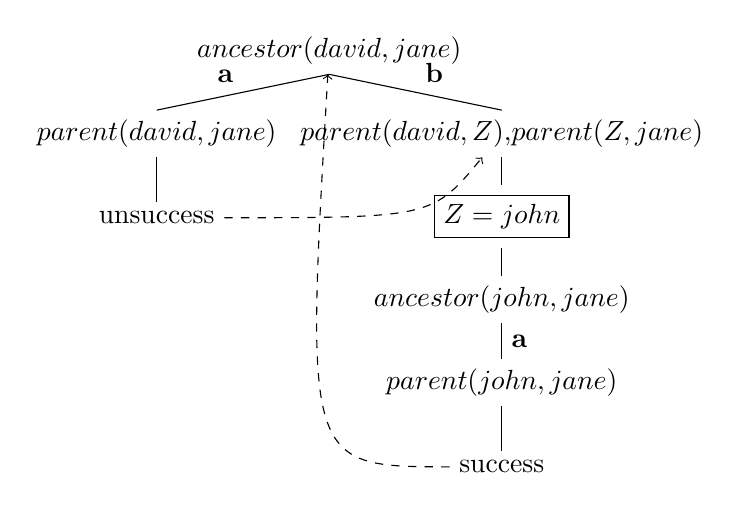
\begin{tikzpicture}


%\tikzset{level distance=42pt}

\Tree [.\node(xh){$ancestor(david, jane)$}; \edge
node[auto=right]{\textbf{a}};[\node(t){unsuccess}; ] .{$parent(david, jane)$}
\edge node[auto=left]{\textbf{b}}; [ [[\edge
node[auto=left]{\textbf{a}};[\node(u){success}; ].{$parent(john, jane)$}
].{$ancestor(john, jane)$} ]  .\fbox{$Z = john$} ].\node(wh){$parent(david, Z),$\\ $parent(Z, jane)$};] 
\draw[dashed,->] (t)..controls +(east:3.5) .. (wh);
\draw[dashed,->] (u)..controls +(west:2.5)  .. (xh);
\end{tikzpicture}
%\end{center}
\caption{Expression evaluation in Prolog}

\end{figure}



First of the queries is answered unsuccessfuly when applied rule \textbf{a},
rule \textbf{b} is then successful.


%*****************************************************************************
\chapter{Meaning of annotations}

\section{Introduction}
Annotations are tags that programmer insert into source code so that they
can be processed by tools. The Java compiler understands a couple of
annotations, but to go any further, you need to build your own processing tool
or obtain a tool from a third party. Most common use of annotations are
\cite{horstmannCornell:coreJava}:

\begin{itemize}
  \item Automatic generation of auxiliary files, such as deployment descriptors or bean information classes.
  \item Automatic generation of code for testing, logging, transaction semantics, and so on.
\end{itemize}

In EJB 3.0 are annotations used in such sense, that a lot of repetitive code is
automated by annotations.

\section{Annotations as metadata}
Metadata are data about data. In context of computer program, metadata are data
about the code. Since Java 5.0 release, programmer can insert arbitrary data
into his source code \cite{java:annotations}. Annotations in Java is used like
an \textit{modifier}, placed before annotated item (it is a keyword similar to \verb|public| or
\verb|static|). Annotations are used to annotate classes, fields or local
variables and can be processed by tools that read them.

Each annotation is declared by annotation interface correspond to the element of
the annotation.

Annotations do not directly affect program semantics, but they do affect the way
programs are treated by tools and libraries, which can in turn affect the
semantics of the running program. Annotations can be read from source files,
class files, or reflectively at runtime.

\section{Examples of use}

\subsection{Field validation}

Annotation type declarations are similar to normal interface declarations. An
at-sign (\verb|@|) precedes the \verb|interface| keyword. Each method
declaration defines an \textit{element} of the annotation type. Method
declarations must not have any parameters or a \verb|throws| clause. Return
types are restricted to primitives, \verb|String|, \verb|Class|, \verb|enums|,
annotations, and arrays of the preceding types. Methods can have default values.
Here is an example annotation type declaration:

\lstinputlisting[label=samplecode,caption=Length annotation]{src/Length.java}

Annotations can be annotatied itself. Such annotations are called
\textit{meta-annotations}. E.g. using
(\verb|@Target(ElementType.FIELD)|) indicates, that annotation type should
be used to annotate only field declarations.
This simple annotation is typically used for entity field e.g. of type
\verb|String| for permitted length of this field.

Once an annotation type is defined, you can use it to annotate declarations. An
annotation is a special kind of modifier, and can be used anywhere that other
modifiers (such as \verb|public|, \verb|static|, or \verb|final|) can be used.
By convention, annotations precede other modifiers. Annotations consist of an at-sign
(\verb|@|) followed by an annotation type and a parenthesized list of
element-value pairs. The values must be compile-time constants. Here is a filed
declaration with an annotation corresponding to the annotation type declared above:

\lstinputlisting[label=samplecode,caption=Class Role]{src/Role.java}

Annotation type without any elements is called \textit{marker}
annotation type, e.g.:

\lstinputlisting[label=samplecode,caption=Entity annotation]{src/Entity.java}

We can join these two types of annotation together in following example:

\lstinputlisting[label=samplecode,caption=Entity Role]{src/entity/Role.java}

Another type of meta-annotation
(\verb|@Target(ElementType.METHOD)|) is presented below and indicates using
annotation only for method declarations:

\lstinputlisting[label=samplecode,caption=Test annotation]{src/Test.java}

In following example, there is updated entity shown above with tool for testing
the annotations:
\lstinputlisting[label=samplecode,caption=Extended class
Role]{src/extended/Role.java}
\lstinputlisting[label=samplecode,caption=Test of method
annotation]{src/RunTests.java}
\newpage
\lstinputlisting[label=samplecode,caption=Test of entity
Role annotation]{src/TestRole.java}


\subsection{Annotating Event Handlers}
In this subsection is shown example presented in
\cite{horstmannCornell:coreJava}. When programmer have to use in his code action
listeners, it leads to write a lot of repetitive code. Listeners are usually declared:

\lstinputlisting[label=listener,caption=Action
listener]{src/listeners/Button.java}

Writing this boring code can be omitted by using annotations. Annotation will
have form:

\lstinputlisting[label=listenerAnnotation,caption=Annotation for
performing action]{src/listeners/AnnotationAction.java}

Instead of calling action listener is every method tagged with annotation.

\lstinputlisting[label=usingListenerAnnotation,caption=Use annotation for
performing action]{src/listeners/ButtonTest.java}

\lstinputlisting[label=ActionListener,caption=Declaration of annotation for
performing action]{src/listeners/ActionListenerFor.java}

We now need a mechanism to analyze them and install action listeners. That is
the job of the \verb|ActionListenerInstaller| class. The \verb|ButtonFrame|
constructor calls

\lstinputlisting[label=ActionListener,
caption=Action Installer invocation]{src/listeners/InstallerCall.java}

The static \verb|processAnnotations| method enumerates all methods of the object
that it received. For each method, it gets the \verb|ActionListenerFor|
annotation object and processes it.

Here, we use the getAnnotation method that is defined in the
\verb|AnnotatedElement| interface. The classes \verb|Method|,
\verb|Constructor|, \verb|Field|, \verb|Class|, and \verb|Package| implement
this interface. The name of the source field is stored in the annotation object.
We retrieve it by calling the \verb|source| method, and then look up the
matching field.

\lstinputlisting[label=findingField,
caption=Looking up for field]{src/listeners/FindingField.java}

For each annotated method, we construct a proxy object that implements the\\
\verb|ActionListener| interface and whose \verb|actionPerformed| method calls
the annotated method. The details are not important. The key observation is that the functionality of the annotations was established
by the \verb|processAnnotations| method.
In Example \ref{actionListenerInstaller}, the annotations were processed at run
time. It would also have been possible to process them at the source level. A
source code generator might have produced the code for adding the listeners.
Alternatively, the annotations might have been processed at the bytecode level.
A bytecode editor might have injected the calls to \verb|addActionListener| into
the frame constructor.
\newpage
\lstinputlisting[label=actionListenerInstaller,
caption=Action Listener Installer class]{src/listeners/ActionListenerInstaller.java}
%*****************************************************************************
\chapter{Framework description}
\label{chap:framework}
\section{Introduction}
\subsection{Overview}
Squander is a framework providing unified environment for both declarative
constraints and imperative statements in single program. This is very practical when
implementing problems, which are easy to define but difficult to solve them
algorithmically. In such cases, declarative constraints can be natural way to
express problem, whereas imprative code is used for setting up the problem and
data manipulation.

Thanks to ability of mixing imperative code with executable declarations, it is
possible to express problem in terms of existing data structures and then run
framework solver, which according to given constraints update the heap to
reflect the solution.


Without having technology like this one, programmer has to translate his program
to external solver, then run the solver and then again manually translate the
solution back to the native programming language.

\subsection{Architecture}
We can divide running of Squander in following steps:
\begin{enumerate}
  \item serialize heap into relations
  \item translate specs and heap relations into Kodkod
  \item translate relational into boolean logic
  \item (if a solution is found) restore relations from boolean assignments
  (if a solution is found) restore field values from relations
  \item (if a solution is found) restore the heap to reflect the solution
   
\end{enumerate}
\begin{figure}[ht]
\begin{center}
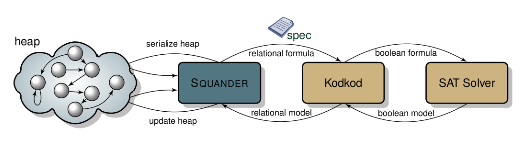
\includegraphics[width=7cm]{figures/architecture-diagram}
\caption{Architecture diagram}
\label{fig:architecture}
\end{center}
\end{figure}

Further will be explained in deatil all of these steps and terms like Kodkod
etc.

\subsection{Applications}
\label{sub:apps}
In this section will be briefly described applications of framework. Most
typical applications are these:
\begin{itemize}
  \item \textbf{solving hard constraint problems} - puzzles (solitaire, sudoku,
  n-queens,\ldots), graph problems (traveling salesman problem, Hamiltonian
  path, general bisection breadth,\ldots), schedulers, dependency managers,\ldots
  \item \textbf{test input generation} - e.g. generate data structure instances
  that satisfy complex constraints
  \item \textbf{specification validation} - specifications can also contain
  errors, and the most intuitive way to test a specification would be to execute
  it on some concrete input and see if the result makes sense or not
  \item \textbf{runtime assertion checking} - check whether a given rich
  property holds at an arbitrary point during the execution of a program
\end{itemize}

On the other hand, framework has some limitations:
\begin{itemize}
  \item \textbf{boundedness} - everything has to be bounded $\rightarrow$ framework
  cannot generate an arbitrary set of new objects (which may be needed to satisfy a
  specification); instead, the exact number of new objects of each class must be
  specified by the user
  \item \textbf{small integers} - integers must also be bounded to a small
  bitwidth (to make the solving tractable), which can occasionally cause subtle
  integer overflow bugs, which are typically hard to find
  \item \textbf{equality issues} - referential equality is used by default for
  all classes except for \verb|String|, so it is impossible to write a spec that
  asserts that two objects are equal in the sense of Java \verb|equals|
  \item \textbf{lack of support for higher-order expressions} - it is not
  possible to write a specification that says \uv{find a path in the graph such
  that there is no other path in the graph longer than it} and solve it with
  Squander; it is possible, however, to express and solve \uv{find a path in the
  graph with at least k nodes}, which is computationally as hard as the previous
  problem, because a binary search can be used to efficiently find the maximum k
  for which a solution exists
 
 
\end{itemize}

\section{Execution of Squander}

Information about framework presented in this section are taken from
\cite{milicevic:executableSpecificationsForJavaPrograms}, where is
thre background of Squander described in detail.

\subsection{Kodkod}
Kodkod is a solver for relational logic. Kodkod requires bounded universe , a
set of untyped relations, bounds for every relation and relation formula. Then
translates given problem into boolean satisfiability problem (SAT) and applies
of-the- shelf SAT solverto search for satysfiyng solution, which is reflected
back if found.

When are the relations in Kodkod created, they are untyped, meaning that every
relation can potentionally contain any tuple drawn from the finite universe.
Actual set of tuples, which relation actually may contains is defined through
Kodkod \textit{bounds}:
\begin{itemize}
  \item \textit{lower bound} to define tuples, that relation \textbf{must}
  contain.
  \item \textit{upper bounds} to define tuples, which relation \textbf{may}
  contain.
\end{itemize}

The size of these bounds has a big influence on search time - the fewer tuples
are in the difference of lower and upper bound, the smaller search space is, the
faster solving is.


\subsection{JFSL}
JSFL is formal lightweight specification for Java supporting relational and set
algebra, as well as common Java operators. Using expressive power of relation
algebra, JFSL makes it easy to succinctly and formally specify complex
properties about Java programs such as method pre and postcondition, class
invariants and so called \textit{frame conditions}, which means portion of the
heap, that is methos allow to modify. It also supports \textit{specification
fields} which can be useful for specifying abstract data types. 


\subsubsection{JFSL expressions}

JFSL expressions are evaluated into relations. JFSL provides common algebra
operators, together with interger and boolean operators. Some of them are shown
in Table \ref{tab:unaryExpressions} and quantified operators, which are also
provided by the framework, are shown in Table \ref{tab:quantifiedExpressions}.


\begin{table}[ht]
  \centering
  
  \begin{tabular}{|l|l|}
  \hline
  \rowcolor[gray]{.8}    Operator  & Description  \\
  \hline
  \hline
  \verb|#| & set cardinality\\
  \hline
  \hline
  \verb|no| & \uv{no} multiplicity (empty)\\ 
  \hline
  \verb|lone|  & \uv{lone} mulitiplicity (zero or one)\\ 
  \hline
  \verb|one| & \uv{one} multiplicity (exactly one) \\ 
  \hline
  \verb|some| & \uv{some} multiplicity (one or more) \\ 
  \hline
  \verb|!| & boolean negation \\ 
  \hline
  \verb|-| & integer negation \\ 
  \hline
  \verb|sum| & integer summation \\ 
  \hline
  \hline
  \verb|=>| & boolean implication \\ 
  \hline
  
  \verb|<=>| & boolean equivalence (\uv{if and only if}) \\ 
  \hline
  \hline
  \verb|?| & if-then-else ternary operator (as in Java) \\ 
  \hline
  \hline
  \verb|@+| & relational union \\ 
  \hline
  \verb|@-| & relational difference \\ 
  \hline
  \verb|@&| & relational intersection \\ 
  \hline
  \end{tabular}
  \caption{Unary expressions supported by JFSL}
  \label{tab:unaryExpressions}
\end{table}

\begin{table}[ht]
  \centering
  
  \begin{tabular}{|l|l|l|}
  \hline
  \rowcolor[gray]{.8}    Operator  & Description  & Usage\\
  \hline
  \hline
  \verb|all| & universal quantifier & \verb#all x: T | P(x)#\\
  \hline
  \verb|some| & existential quantifier & \verb#some x: T | P(x)#\\ 
  \hline
  \verb|sum|  & integer summation & \verb#sum i: int | a[i]#\\ 
  \hline
  \verb|union| & set comprehension & \verb#{x: T | P(x)}#\\ 
  \hline
  
  \end{tabular}
  \caption{Quantified expressions supported by JFSL}
  \label{tab:quantifiedExpressions}
\end{table}
\newpage
\subsubsection{JFSL annotations}
JFSL annotations are written as Java annotations and are for interaction
between framework and programmer. Main components (JFSL annotations) are:

\begin{itemize}
  \item \verb|@Invariant| - this annotaion is attached to the classes and used
  to define, that condition must be fulfilled for the given class. That means,
  that this condition has to be fulfilled before and after execution.
  
  \item \verb|@Requires| -  this annotation specifies constraints before method
  invocation. The method is expected to execute correctly if only the
  precondition is satisfied immediately before method invocation. Class
  invariants are added immediately to the method preconditions.
  \newpage
  \item \verb|@Ensures| - attached to the methods and used to specify
  constraints on the state, which have to be satisfied after method invocation.
  It means, that it captures all effect that method is expected to produce.
  Class invariants are implicitly added to method postconditions.
  
  \item  \verb|@Modifies| - this annotation is attached to the methods to
  specify frame conditions. Frame condition can hold up 4 different pieces of
  specification (syntax: \verb|@Modifies| \verb|("f [s][l][u]")|). First, and
  the only one mandatory piece, is the name of modifiable field, \verb|f|. It is
  optionally followed by \textit{instance selector} \verb|s|, followed by
  \textit{lower bound} and the \textit{upper bound}. Instance selector specifies
  instances, for which the field may be modified - if not specified, it is
  assumed \uv{all}. The lower bound contains concrete field values for some
  objects in the post-state. The upper bound holds the possible field values in
  the post-state.
  
  \item \verb|@SpecField| - attached to the classes and used to define
  specification fields. Definition of type specification consists of type
  declaration, and optionally an abstract function. the abstraction function
  defines, how the field value is computed in terms of other fields. For example
  \verb#@SpecField("x: one int| x = this.y - this.z")#  defines a singleton
  integer field \verb|x|, the value of which must be equal to the difference of
  \verb|y| and \verb|z|. Specifications fields are inherited from super-types
  and sub-types can override the abstraction function (by simply redefining
  it), a feature that is particularly useful for specifying abstract datatypes,
  such as Java collections.
  
  

  
\end{itemize}

In context of these specification, the goal is to execute a method, that makes
modification of the portion of the heap (specified in frame condition), so that
final state satisfies postcondition.

\subsection{From object heap to relational logic}

Execution of Squander begins in client's code when invoking
method \verb|Squander.exe()| involving following steps:

\begin{enumerate}
  \item Assembling all revelant constraints from annotations, as well as class
  annotations corresponding to all invariant classes.
  \item Construction relations representing objects and their fields in
  pre-state and adding additional relations for holding their values in the
  post-state, along with their Kodkod bounds
  \item Parsing constraints and converting them to a single relational formula
  \item If solution is found, translation of the Kodkod result objects into
  updates of Java heap state, by modification of the object fields
\end{enumerate}

\subsubsection{Traversing the heap}

For discovering reachable portion of the heap, bread-first search algorithm is
used, which started from the set of root objects and repeatedly visiting all
children until all reachable objects have been visited. The most important part
is how to enumerate childre, i.e. how to serialize a given object into a set of
field values.

\subsection{Relations and bounds}
After traversing the heap, founding all reachable objects and
discovered all classes/-fields reffered in the specification, we have enough
information to construct the relation, that represent state of the heap.

The translation does not used all fields, but only those, whose are considered
as \textit{relevant fields} - those, who are explicitly mentioned in the
specification (Squander's annotation). Similarly, not all reachable objects are
needed; only objects reachable by following the relevant fields are included in
the translation. These objects will be referred to as \textit{literals}.

First we define a finite universe consisting of all literals, plus integers within the
bound. For every literal, a unary relation is created.

For each Java type, one could either create a new relation (with appropriate
bounds so that it contains the known literals), or one could construct a relational
expression denoting the union of relations corresponding to all instance literals of that
type.


For every field, a relation of type
\verb|fld|$.declType \rightarrow$ \verb|fld|$.type$ is created to hold
assignments of field values to objects. If the field is modifiable (inferred
from its mention in a \verb|@Modifies| clause), an additional relation is
created, with the suffix \uv{pre} appended to denote the pre-state value.
Relations for unmodifiable fields are given an exact bound that reflects the
current state of the heap. For the modifiable relations, the \uv{pre} relation
is given the same exact bound, and the “post” relation is bounded so that it may
contain any tuple permitted by the field's type. Local variables, such as
\verb|this|, \verb|return|, and method arguments are treated similarly to
literals.

\newpage

Table \ref{tab:translationsToRelations} below summarizes how relations and
bounds are created. Function \verb|rel| takes a Java element and, depending
whether the element is modifiable, returns either one or two relations. Function
\verb|bound| takes a Java element and its corresponding relation, and returns a
bound for the relation. The \verb|Bound| data type contains both lower and upper
bounds. If only one expression is passed to its constructor (\textbf{B}), both
bounds are set to that value. Helper functions \verb|is_mod|, \verb|is_post|
and \verb|fldval| are used to check whether a field is modifiable, to check
whether a relation refers to the post-state, and to return a literal that
corresponds to the value of a given field of a given literal, respectively.


\begin{table}[ht]
  \centering
  
  \begin{tabular}{|l|l|l|}
  \hline
  \rowcolor[gray]{.8}   \textbf{rel} :: Element $\rightarrow [$Relation$]$\\
  \hline
  \hline
  
  \textbf{rel} (Literal lit) \hspace{31mm} $=$ \hspace{2mm} $
  [$\textbf{R}(lit.$name$, lit.$type$)$]$ \\
  \textbf{rel} (Type t)\hspace{37mm} $=$ \hspace{2mm} $ 	\bigcup_{lit<:t}$
  \textbf{rel} lit\\ \textbf{rel} (Field fld) \hspace{33.1mm} $=$ \\
\hspace{2mm}	\textbf{if} is\_ mod(fld)\\
\hspace{10mm} $[$\textbf{R}(fld.$name$, fld.$declType \rightarrow
$fld.$type$)$]$ ++\\ 
\hspace{10mm} $[$\textbf{R}(fld.$name$ + \_pre, fld.$declType \rightarrow
$fld.$type$)$]$\\ 
\hspace{5mm} \textbf{else}\\
\hspace{10mm} $[$\textbf{R}(f.$name$, f.$declType \rightarrow $f.$type$)$]$\\
\textbf{rel} (Local var)\hspace{34mm} $=$ \hspace{2mm} $
[$\textbf{R}(var.$name$, var.$type$)$]$\\
 
  \hline
  \hline
  \rowcolor[gray]{.8}   \textbf{rel} :: Element, Relation $\rightarrow
  [$Bound$]$\\
  \hline
  \hline
  
  \textbf{bound} (Literal lit) (Relation r) \hspace{5.2mm} $=$ \hspace{2mm} 
  \textbf{B}(lit) \\
  \textbf{bound} (Field f) (Relation r) \hspace{10mm} $=$ \\ 
  \hspace{5mm}	\textbf{if} is\_ mod(fld) $\wedge$ is\_post(r)\\

\hspace{10mm} $[$\textbf{B}(\{\}, ext(fld.$declType \times
$fld.$type$))$]$\\ 

\hspace{5mm} \textbf{else}\\
\hspace{10mm} $[$\textbf{B}($ 	\bigcup_{lit<:Object}$
  \textbf{rel} lit $\times$ fldval(lit,fld))$]$\\\textbf{bound}
  (Return ret) (Relation r)\hspace{5mm} $=$ \hspace{2mm} $[$\textbf{B}(\{\},
  ext(ret.$type$))$]$\\
 \textbf{bound}
  (Local var) (Relation r)\hspace{7mm} $=$ \hspace{2mm} $[$\textbf{B}(var)$]$\\
  \hline
  \hline
  \rowcolor[gray]{.8}   $[$Type$]$ $\rightarrow$
  Expression \hspace{40mm} (hepler)\\
  \hline
  \hline
  
  \textbf{ext} $[]$ \hspace{49.5mm} $=$ \hspace{2mm} \{\}\\ 
  \textbf{ext} (t:$[]$)  \hspace{44mm} $=$ \hspace{2mm} $ \bigcup_{lit<:t}$
  lit\\ \textbf{ext} (t:xs) \hspace{42.5mm} $=$ \hspace{2mm} \textbf{ext} t
  $\times$ \textbf{ext} xs\\
  \hline
  
  \end{tabular}
  \caption{Translation of different Java constructs into relations (function
  \texttt{rel}) and bounds (function \texttt{bound})}
  \label{tab:translationsToRelations}
\end{table}

\newpage
\subsection{Example: translation of \texttt{BST.insert}}
\label{sub:translation}
We will use for illustration of translation Binary Search Tree example. This BST
has single root node. Every node contains integer key value and pointer to the
left and right node. To verify validity of BST, some Squander's specifications
are used (see Listing \ref{bst}). \verb|@SpecField| constraint declares, that
set of BST nodes consist of root node and all nodes in left and right subtree of this root node except
for \verb|null| values. Another constraints represented by \verb|@Invariant|
annotation delares: (1) there are no loops in BST - using transitive closure to
define, that actual node is not accessible transitively via field \verb|parent|
- and (2) and for every node $n$ in the BST, the $key$ of $n$ is strictly greater,
than all keys of all nodes in the left subtree and strictly lower than all keys
of all nodes in its right subtree - there is used reflexive transitive closure
operator (\verb|.*|) to conveniently specify all reachable nodes starting from
the root node.


\lstinputlisting[label=bst,caption=Binary Search Tree
declaration]{src/bst/BST.java}

Methods for modifying tree, \verb|insert()| and \verb|remove()| shown in
Listing \ref{operation} are obvious. In order to insert node into tree, node
with same key may not exist in the tree, and after the insertion, tree must
contain the given node. All left and right pointers of nodes and pointer to root
node are allowed to modify. Deletion is defined in similar way, BST must contain node
with the same key as node to remove and after deletion this node may not exist
in BST.
\newpage
\lstinputlisting[label=operation,caption=Operations on
BST]{src/bst/Operations.java}

The resulting set of relations, shown in Table \ref{fig:translationTable}, are
divided into three sections. Relations in the upper section are unary, unmodifiable relations,
and represent objects on the heap. The middle section contains relations that
are also unmodifiable, because they are used to either represent unmodifiable
fields or values in the pre-state of modifiable fields. Finally, the relations
in the bottom section represent the post-state of modifiable fields; these are
the relations for which the solver will attempt to find appropriate values. By
default, the lower bound is simply set to an empty set and the upper bound is
the upper bound is set the extent of the field's type.


\begin{figure}[ht]
\begin{center}
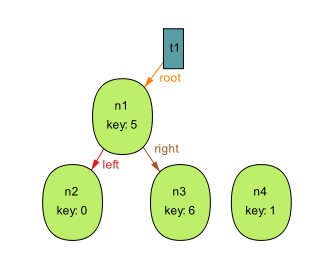
\includegraphics[width=4cm]{figures/bst}
\caption{A snapshot of \texttt{t1.insert(t4)}}
\label{fig:bstInsert}
\end{center}
\end{figure}

\newpage


\begin{table}[ht]
\begin{center}
\begin{tabular}{ l l }
	\textbf{BST}: & $\{t_1\}$\\
	\textbf{N1}: & $\{n_1\}$\\
	\textbf{N2}: & $\{n_1\}$\\
	\textbf{N3}: & $\{n_1\}$\\
	\textbf{N4}: & $\{n_1\}$\\
	\textbf{null}: & $\{null\}$\\
	\textbf{BST\textsubscript{--}this}: & $\{t_1\}$\\
	\textbf{z}: & $\{n_4\}$\\
	\textbf{ints}: & $\{0, 1, 5, 6\}$\\
  \hline
  	\textbf{key}: & $\{(n_1\rightarrow 5),(n_2\rightarrow
	0),(n_3\rightarrow 6),(n_4\rightarrow 1)\}$\\
	\textbf{root\textsubscript{--}pre}: & $\{(t_1\rightarrow n_1)\}$\\
	\textbf{nodes\textsubscript{--}pre}: & $\{(t_1\rightarrow n_1),(t_1\rightarrow
	n_2),(t_1\rightarrow n_3),(t_1\rightarrow n_4)\}$\\
	\textbf{right\textsubscript{--}pre}: & $\{(n_1\rightarrow n_2),(n_2\rightarrow
	0),(n_3\rightarrow null),(n_4\rightarrow null)\}$\\
	\textbf{left\textsubscript{--}pre}: & $\{(n_1\rightarrow n_3),(n_2\rightarrow
	0),(n_3\rightarrow null),(n_4\rightarrow null)\}$\\
	\hline
	\textbf{root}: & $\{\},\hspace{4mm}\{t_1\}\times\{n_1,n_2,n_3,n_4\}$\\
	\textbf{nodes}: & $\{\},\hspace{4mm}\{t_1\}\times\{n_1,n_2,n_3,n_4\}$\\
	\textbf{left}: &
	$\{\},\hspace{4mm}\{n_1,n_2,n_3,n_4\}\times\{n_1,n_2,n_3,n_4\}$\\
	\textbf{right}: &
	$\{\},\hspace{4mm}\{n_1,n_2,n_3,n_4\}\times\{n_1,n_2,n_3,n_4\}$\\
	
\end{tabular}
\end{center}
\caption{Translation of the heap from Figure \ref{fig:bstInsert}}
\label{fig:translationTable}
\end{table}

\subsection{Tightening the bounds}
By declaring as modifiable fields \verb|left| and \verb|right|, as in the
specification in \ref{bst}, we allow arbitrary modifications to the tree, as
long as all constraints are satisfied. In effect, after the execution of the
specification for the \verb|insert()| method, the tree will contain all old
nodes plus the new node, but the shape of the tree may randomly change.

If we want to change method specification so, that tree topology is preserved
and new nodes can be append only to leaf nodes, we can do that by adding new
clauses to the postcondition specification in sense, that left and right
pointers of certain nodes must remain the same in the post state. This idea is
completely right, but more efficient would to change the frame condition also
for improving performance. Reducing search space by allowing modification only
\verb|left| and \verb|right| pointers pointing to \verb|null| value improve
performance significantly.

Consider modified frame condition shown in Listng \ref{modifiedOperation}
specifying additional constraints on the modification of \verb|left| and \verb|right| fields. This
frame condition shows idea specified in paragraph before and ensures, that all
new nodes will be inserted at the leaf positions.

\lstinputlisting[label=modifiedOperation,caption=Modified
frame condition on \texttt{insert()} method]{src/bst/ModifiedOperations.java}

With the list of modifiable objects, Squander modifies the bounds for the
corresponding field relation so that the current field values of the objects not
to be modified are included in the lower bound, thus forcing the value to stay
the same in the post state. For the heap shown in Figure \ref{fig:bstInsert},
the modifiable objects for the \verb|left| field are \verb|n2| and \verb|n3|,
because their left pointers are currently set to null. Similarly, for the
\verb|right| field, the modifiable objects are also \verb|n2| and \verb|n3|. The
updated bounds for these two fields are shown in Table \ref{fig:updatedBounds}.


\begin{table}[ht]
\begin{center}
\begin{tabular}{ l l }
	\textbf{left}: &
	$\{(n_1\rightarrow
	n_2),(n_4 \rightarrow
	null)\},\hspace{4mm}(n_1 \rightarrow n_2)\cup(n_4 \rightarrow
	null)\cup \{n_2,n_3\}\times\{n_1,n_2,n_3,n_4\}$\\ 
	\textbf{right}: &
	$\{(n_1\rightarrow
	n_3),(n_4 \rightarrow
	null)\},\hspace{4mm}(n_1 \rightarrow n_3)\cup(n_4 \rightarrow
	null)\cup \{n_2,n_3\}\times\{n_1,n_2,n_3,n_4\}$\\
	
\end{tabular}
\end{center}
\caption{The updated bounds for the \texttt{left} and \texttt{right} relations}
\label{fig:updatedBounds}
\end{table}

\subsection{Minimizing the universe size}
\label{sub:minUniverse}
For representing relations in Squander are used single sequential arrays indexed
by Java integer. Maximal count of members in this array is \verb|Integer.MAX_VALUE| which is
$2147483647$. In practice this can be a problem, because framework for relation
of arity $k$, which has $n$ atoms in the universe (later it will be described,
what is exactly meant under this term), allocates matrix of size $n^k$ (when
ternary relation contains more than 1290 atoms). Heap with more than 1290
objects are not uncommon, so a simple translation described in
\ref{sub:translation} would not work. In the next subsection will be described a
different translation technique called \textit{KodkodPart}, which was developed
to minimize number of atoms representing object heap.

\subsubsection{\textit{KodkodPart} translation}
\label{sub:kodkodpart}
KodkodPart translation achieves a universe with fewer atoms by mapping
Java objects to Kodkod atoms (not injective mapping). That means that multiple
literals are mapped to a single atom, so that there will be fewer atoms than
literals. The key requirements is, that there exists some inverse function,
which maps back from the atoms literals.

Considering previous example with BST (see subsection \ref{sub:translation}), we
can define domains $\mathcal{D}$, literals $\mathcal{L}$ and assignment literals to domains
$\gamma : \mathcal{D} \rightarrow \mathcal{P}\left(\mathcal{L}\right)$ for this
example, which is summarized in Table \ref{tab:summaryDomainsLiterals}.

\begin{table}[ht]
\begin{center}
\begin{align*}
	\mathcal{D}& =\{\texttt{BST},\hspace{1mm} \texttt{Node},\hspace{1mm}
	\texttt{Null}, \hspace{1mm} \texttt{Integer}\}\\ 
	\mathcal{L}& =\{bst_1,\hspace{1mm} n_1,\hspace{1mm} n_2,\hspace{1mm}
	n_3,\hspace{1mm} n_4, \hspace{1mm} null,\hspace{1mm} 0,\hspace{1mm} 1,\hspace{1mm} 5,\hspace{1mm} 6\}\\
	\gamma\left(\texttt{BST}\right)& = \{bst_1\}\\
	\gamma\left(\texttt{Node}\right)& =
	\{n_1,\hspace{1mm}n_2,\hspace{1mm}n_3,\hspace{1mm}n_4\}\\
	\gamma\left(\texttt{Null}\right)& =
	\{null\}\\
	\gamma\left(\texttt{Integer}\right)& =
	\{0,\hspace{1mm}1,\hspace{1mm}5,\hspace{1mm}6\}\\
\end{align*}
\end{center}
\caption{Summary of domains and instances for the \texttt{BST.insert} example}
\label{tab:summaryDomainsLiterals}
\end{table}

Recall that field types are represented as unions of base types (in this section also
called \textit{partitions}). For instance, the type of the field \verb|BST.root|
is \verb|BST| $\rightarrow$ \verb|Node| $\cup$ \verb|Null|, because values of
this field can be either instances of \verb|Node| or the \verb|null| constant.
That means that all objects of class \verb|Node| plus the constant \verb|null|
must be mapped to different atoms, so that it is possible to unambiguously
restore the value of the field \verb|root|. This is the basic idea behind the
KodkodPart translation: \textit{all literals within any given partition must be
mapped to different atoms, whereas literals not belonging to a common partition may
share atoms}. The inversion function can then work as follows: for a given atom,
first select the correct partition based on the type of the field being
restored, then unambiguously select the corresponding literal from that
partition. To complete the example, the set of all unary types used in the
specification for this example is:

\begin{center}
\begin{align*}
	\mathcal{T}& =\{\texttt{BST},\hspace{1mm}
	\texttt{BST}\cup\texttt{Null},\hspace{1mm} \texttt{Node} \cup \texttt{Null},
	\hspace{1mm} \texttt{Null},\hspace{1mm} \texttt{Integer}\}\\
\end{align*}
\end{center}

Set presented above is set of our partitions. A valid assignment of
atoms to literals that uses only 5 atoms, as opposed to 10 which is how many the
original translation would use, could be:

\begin{center}
\begin{tabular}{|l|l|l|l|l|}
  \hline
  $bst_1 \rightarrow a_0$ & $n_1 \rightarrow a_0$ & $n_2 \rightarrow a_1$ & $n_3
  \rightarrow a_2$ & $n_4 \rightarrow a_3$\\
  \hline
  $null \rightarrow a_4$ & $0 \rightarrow a_0$ & $1 \rightarrow a_1$ & $5
  \rightarrow a_2$ & $6 \rightarrow a_3$\\
  \hline
  \end{tabular}
\end{center}

Limitation of this technique is when the class \verb|Object| is used as a field
type or anywhere in the specification. This lead toone big partition containing
all literals (because every class is a subclass of \verb|Object|), making the
algorithm equivalent to the original translation.

\subsubsection{Partitioning algorithm}
For a given set of base domains $\mathcal{D}$, literals $\mathcal{L}$, and
partitions $\mathcal{T} \left( \mathcal{T} = \mathcal{P}\left( \mathcal{D} \right) \right)$, and a given function $\gamma : \mathcal{D} \rightarrow \mathcal{P}\left( \mathcal{L} \right)$ that maps domains to their instance
literals, this algorithm produces a set of atoms $\mathcal{A}$ and a function $\alpha : \mathcal{L} \rightarrow \mathcal{A}$, such that for every partition
$p$, function $\alpha$ returns different values for all instance literals of
$p$. Formally:

$$\left(\forall p \in \mathcal{T}\right)\left(\forall l_1,l_2 \in
\psi\left(p\right)\right) l_1 \neq l_2 \Longrightarrow \alpha
\left(l_1\right)\neq \alpha \left(l_2\right)$$


where $\psi$ is a function that for a given partition returns a comprehension of
all instance literals of all of its domains:


$$\psi : \mathcal{T}\rightarrow \mathcal{P} \left(\mathcal{L}\right);
\hspace{2mm} \psi\left(p\right) = \{\gamma\left(d\right)\mid d \in p\}$$

Obviously, a simple bijection would satisfy this specification, but such a solution
wouldn't achieve its main goal, which is to minimize the number of atoms, because
the number of atoms in this case would be exactly the same as the number of literals.
In order to specify solutions that are actually useful, we are going to require the
algorithm to produce a result such that the cardinality of $\mathcal{A}$ (i.e.
the total number of atoms) is minimal.

It is not immediately clear what the minimal number of atoms ought to be. One
might think that no more atoms are required than the number of instances in the
largest partition. However, this is not always true. Consider the case shown in
Figure \ref{fig:kodkodpart}. The largest partitions are \verb|P1| and \verb|P4|,
both having 5 literals. On the other hand, any pair of the domains \verb|B|, \verb|C|, and
\verb|D| have a partition in common, even though there is no single partition
containing them all. They thus form a strongly connected component, and their literals must differ. There are 6 literals in total in
these three domains, so 5 atoms cannot be enough. As a conclusion, the minimal
number of atoms is indeed the number of literals in the largest partitions, but only
after all strongly connected domains have been merged into a single partition.


\begin{figure}[ht]
\begin{center}
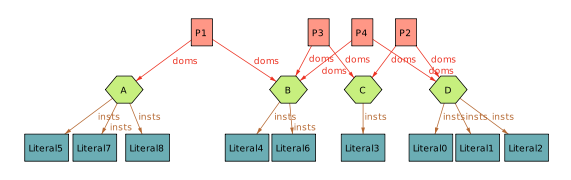
\includegraphics[width=8cm]{figures/kodkodpart}
\caption{KodkodPart: an example where more than the number of literals of the
largest partition is needed.}
\label{fig:kodkodpart}
\end{center}
\end{figure}

Luckily, cases like the one in Figure \ref{fig:kodkodpart} never happen in
Squander, so our implementation of the algorithm doesn't have to search for
cliques and merge partitions. The reason this never happens is that domains are
always Java classes, and partitions are types used to represent fields. A type
of a field is a union type which includes the entire subclass hierarchy of the
field’s base type. For instance, if \verb|C| and \verb|D| are Java classes,
\verb|C| extends \verb|D (C <: D)|, and some field has declared type \verb|D|,
then the type of the field (in the relational world) will be \verb|D| $\cup$
\verb|C| $\cup$ \verb|Null|, meaning that \verb|D| $\cup$ \verb|Null| is
never going to be used as a partition for anything.

In summary, the actual implementation inside Squander works as follows:


\begin{enumerate}
  \item Dependencies between domains are computed. A domain depends on all
  domains with which it shares a partition. Let the function $\delta :
  \mathcal{D} \rightarrow \mathcal{P}\left(\mathcal{D}\right)$ express this:
  
  $$\delta\left(d\right) = \{d_1 \mid d_1 \neq d\ \wedge
  \left(\left(\exists p \in \mathcal{T}\right)d_1 \in p\right)\} $$
  \item The largest partition $p_{max}$ is found such that
  $$\left(\nexists p\in \mathcal{T}\right) \abs{\psi\left(p\right)} >
  \abs{\psi\left(p_{max}\right)}$$
  \item For every literal $l$ in $\psi\left(p_{max}\right)$ an atom a is
  created, it is added to the universe $\mathcal{A}$ and assigned to $l$, such
  that $\alpha\left(l\right) = a$. From this point onwards, $\mathcal{A}$ is fixed.
  \item For every other partition $p$ iteratively, for all literals $l_p \in p$
  that do not already have an atom assigned, a set of possible atoms
  $\mathcal{A}_{lp}$ is computed and the first value from this set is assigned
  to $l_p$. $\mathcal{A}_{lp}$ is computed when atoms corresponding to all literals of all
  dependent domains is subtracted from $\mathcal{A}$, i.e.:
  \newpage
  
  $$\mathcal{A}_{lp} = \mathcal{A} \setminus \{\alpha\left(l\right)\mid
  l\in\mathcal{L}_d\} \text{, where}$$
  
  $$\mathcal{L}_d = \{\gamma\left(d\right)\mid
  d\in\mathcal{D}_d\} \text{, where}$$
  
  $$\mathcal{D}_d = \delta\left(d_l\right) \text{, where } d_l\in\mathcal{D}
  \wedge l_p \in \gamma\left(d_l\right)$$
\end{enumerate}
\section{Differences between Prolog and framework}

Thing, which have both classical logical programming in Prolog and
programming using framework Squander in common, is defining what to compute
instead of how. Both programming paradigms use set of rules for its computation,
but here the analogy ends.

If we study Prolog and Squander more in depth, we can see, that there is
significant difference in declaring input data. Whereas Squander is strongly
connected to its Java data structures, Prolog use set of facts, as was
mentioned in chapter \ref{chap:logProgPrinc}.


Both Prolog and Squander use set of rules for its computation. If we want to
compute some variable in Prolog, language go recursively through all rules,
matching the input using rewriting clauses, until all of them are replaced by
valid facts and we do not care about order of evaluation (no flow control).
Prolog uses three types of formula. \textit{Atomic} formulas declares basic
facts, \textit{conditional commands} are used for implication constructs and
finally, \textit{target clauses} form query types.


To incorporate Squander into Java annotations are used. For solving some
algorithm, annotation \verb|@Requires|,\verb|@Ensures| and \verb|@Modifies| are
mostly used. First one, \verb|@Requires|, is used for declaring requirements for
input data before method \verb|Squander.exe()| is invoked. Annotation
\verb|@Ensures| defines how the data structures should look like after method
execution. Last one, \verb|@Modifies|, tells framework class objects or object's
fields can be modified during execution. This is very important declaration
for the performace of the computation in particular. If we define this
annotation optimally, we minimize search space and speed up solving. Calculation
itself is done by translating object heap into relations. Then are these
relations transformed into SAT problem, which is then solved and the solution,
if exists, is reflected back to the heap.
%*****************************************************************************
\chapter{Implementation of algorithms}

\section{Introduction}
As was mentioned before, framework Squander is suitable for implementation of
algorithms, which are easy to specify, but difficult to implement imperatively.
For this reason I implemented algorithms belonging to NP problems. Problem is
said that belongs to the set of NP problems if it is solveable in polynomial
time on nondeterministic Turing machine. There is one more expression to
explain for description of NP problems - \textit{nondeterministic Turing
machine}. First of all we have to define deterministic Turing machine, which for
given set of rules prescribes at most one action to be performed for any given
situation. Whereas nondetermistic Turing machine is machine, that for given set
of rules prescribes more than one action. We can imagine, that in every step of
computation is Turing machine cloned in nondeterministic Turing machine.

Most of the algorithm I tried to implement are NPO (especially graph
algorithms), but there is a little problem with Squander. It does not support
highr-order expressions (subsection \ref{sub:apps}). Unfortunately it is not
possible to write a specification that says \uv{find a path in the graph such
that there is no other path in the graph longer than it} and solve it with
Squander; it is possible, however, to express and solve \uv{find a path in the
graph with at least k nodes}, which is computationally as hard as the previous
problem, because a binary search can be used to efficiently find the maximum k
for which a solution exists. Due that restriction are all of the optimizations
algorithms implemented in such way, that there is some treshold level, which
solution has to satisfy.


All in all, Squander should be able to solve all NP problems, because it
transforms everything into SAT problem, which is NP-complete (Cook's theorem)
problem and every NP problem is transferable into NP-complete problem.
\section{Knapsack Problem}

\subsection{First version}
At the beginning when I started \uv{playing} with Squander, I tried to
implement optimization variant of well known algorithm Knapsack. This algorithm
is usually introduced, that there is burglar with knapsack inside some estate and he has to steal
as many things as capacity of his knapsack allowed to him with highest price. 

This problem is also sometimes called the easiest one from NP-hard problems. If
we try to solve it by brute force, we get an exponential time complexity. But
there are more than one way how to solve this problem with different complexity.
E.g. by using dynamic programming we get pseudo-polynomial time complexity,
which means that time complexity is depends not only on input data but also on
another variable.

By using Squander's method specification it was pretty easy to declare
annotations for computation. Firstly it was necessary to prepare data
structures. In this case I implement class \verb|KnapSacck.java|, which has
following properties:

\begin{itemize}
  \item \textit{integer array c} - costs of particular things in knapsack
  \item \textit{integer array v} - weights of particular things in
  knapsack
  \item \textit{integer n} - count of things in knapsack
  \item \textit{integer capacity} - capacity of knapsack (measured in weight
  units)
\end{itemize}

That is all information we need to know about object \verb|Knapsack|. Important
thing is to define some treshold - in our case it will be total cost of things
in knapsack, which we pass as parameter. Now we have to define some Squander's
specification. Firstly we make a decision, if configuration of things will be returned as a new array or
if we pass some array as a method parameter. Let us try to choose first option.
This option is connected with annotation \verb|@FreshObjects|, which is used to
define, which type of object will be returned from \verb|Squander.exe()|
method, so one instance of the object \verb|Integer| array should be created on
the heap specifying which things are in the knapsack (value $1$) and which not
(value $0$). After these steps, our method specification looks like this:

\lstinputlisting[label=knapSack1,caption=Declaration of return type of
\texttt{Squander.exe()} method]{src/knapsack/KnapSack1.java}

After that we define some constraints, that help reduce search space. Question
that we must ask is what objects or fields of which classes are allowed to
be modified. Costs and weights are same during computation, similarly capacity
and count of things in knapsack. The only structure that has to be modifiable is
return array of \verb|Integers|. According to Squander's documentation we have
to declare via annotation \verb|@modifies|, that both length and elements of
returned array are modifiable:

\lstinputlisting[label=knapSack2,caption=Definition of modifiable objects on
\texttt{Squander.exe()} method]{src/knapsack/KnapSack2.java}

The next step is to decide if we have some requirements on input data. We can
see that this data are quite enough restricted by its own data type so we do not
use annotation \verb|@Requires|, which is used to define some prerequisities for
the execution. Let us continue with specification what we expected as a result
of computation. 

So the last thing we have to specify is method output. At first come definition,
that total weight of the all things in knapsack has to be smaller or equal to
the knapsack capacity:

\lstinputlisting[label=knapSack3,caption=Declaration of knapsack capacity
constraint on \texttt{Squander.exe()} method]{src/knapsack/KnapSack3.java}

Then it is necessary to specify, that total cost of things in knapsack has to be
greater than varibale \verb|minCost|, which is passed as method parameter:

\lstinputlisting[label=knapSack4,caption=Declaration of knapsack total cost
constraint on \texttt{Squander.exe()} method]{src/knapsack/KnapSack4.java}

It is obvious, that Squander use keyword \verb|this| in similar way as Java.
Finally we make a specification, that length of return \verb|Integer| array has
to be \verb|n| and that values of that arrays have to be from set $\{0, 1\}$:

\lstinputlisting[label=knapSack5,caption=Declaration of parameters of returned
array on \texttt{Squander.exe()} method]{src/knapsack/KnapSack5.java}

Knapsack problem is now completely implemented but let us think about possible
improvements. When thinking about improvement, we should concentrate on
modifiable object, which is returned \verb|Integer| array. In this case we get
by with array of Boolean values, which shrinks variable domain as much as possible
and limit the search space. We have declared constraint in \verb|@Ensures|
annotation, that values of returned array are in set $\{0, 1\}$, but this
constraint does not limit search space. Due that change, we should also modify
declaration of constraints describing minimal cost and capacity of knapsack. It
is necessary also modify \verb|@FreshObject| annotation to Boolean data type.
\newpage
\lstinputlisting[label=knapSack6,caption=Improving
implementation of Knapsack using Boolean data type]{src/knapsack/KnapSack6.java}

Now we have implement Knapsack problem in advanced way and it is time for
testing, if it works correctly. During testing I used instaces for which I
know the \verb|bestPrice| solution and for a treshold \verb|minCost| I used
value equals to \verb|bestPrice - 1|.

At first was the implementation tested on smaller instances consisting of 4
things. From 45 examples was one failed, when Squander returns configuration,
which was overweight. Moreover when was minimal cost greater or eequal to
$512$, program fails on error\\ \verb|Arity too large (3) for a universe of size 2055|. We know
from chapter \ref{chap:framework}, subsection \ref{sub:kodkodpart} that Squander
used for representing relation array indexed by Java integer. Due to size of
the universe $2055^3 = 8678316375$ which is greater than
\verb|Integer.MAX_VALUE| which is $2147483647$ is Squander unable to represent
relation. Why does it happen? If is in the specification \verb|minCost|
greater or equal to $512$, Squander automatically uses $11$ bits to
represent \verb|Integers|, which gives a scope $<-2^{10},2^{10}) =
\{-1024,\ldots,1023\} = 2048$ \verb|Integers| and as was mentioned in subsection
\ref{sub:minUniverse}, these ternary relations cannot be mapped into
\verb|Integer| indexed array $(2048^3 > 2147483647)$. Another problem comes in,
when we variable \verb|minCost| is set to $511$. Then Squander uses bitwidth $10$, which means $<-2^9,2^9) = \{-512,\ldots,511\}$ and that is why it is unable to find solution, which is $512$ so not in the scope, and throws \verb|noSolutionException|.

We can see from the measurement, that this implementation of knapsack
using Squander is for this type of problem quite unsuitable.

\subsection{Second version}

In order to reduce search space, I tried to implement another version of
knapsack problem. Let us think about things in knapsack as an entity, not as a
configuration variable in array. By using this way of thinking, we get reduced
count of atoms in Squander, because now we have only one set of objects \verb|Thing| but in the
first version of implementation there were two arrays of the same data type
(\verb|Integer| array \textit{c} and \verb|Integer| array \textit{v} same size
as set of things we have now), which drastically increase number of atoms.
Fields of entity \verb|Thing| look like this:

\begin{itemize}
  \item \textit{integer c} - cost of actual thing
  \item \textit{integer v} - weight of actual thing
  \item \textit{boolean choosed} - symptom if is choosed
  \item \textit{integer position} - this variable is used for sorting the
  output, because instances of \verb|Thing| are in \verb|java.util.Set|
  (for performance reasons)
\end{itemize}

For a specification of Squander, we create \verb|Set| of objects \verb|Thing|,
allowing to modify only \verb|boolean choosed| symptom. Summation logic is the
same as in first version and variable \verb|position| is used for sorting
resulted set of object in order to have better interpretation of the solution.

In this example we use experience from the previous one and declare variable
\verb|minCost| as the real maximum cost of possible solution and write it to the
specification (sum of cost should be equal to \verb|minCost|), so best
solution value will not disappear in higher \verb|Integer| bitwidth. On the
other hand, this implementation is not very usable, because we almost always do
not know exact highest total price.

\lstinputlisting[label=knapSack7,caption=Improving
implementation of Knapsack using previous
experince and reducing count of relations]{src/knapsack/KnapSack7.java}

This way of implementation is suitable for instances with more things in
knapsack, which means higher value of variable \verb|capacity| and higher value
of variable \verb|minCost|, because there are not so many relations created.
Implementation was successfuly tested for $40$ things in one instance at most.

\section{General bisection breadth}

\label{sec:gbb}
This problem is taken from course \textit{Parallel Systems and Algorithms}
lectured at Faculty of Electrical Engeneering of Czech Technical University in
Prague (CTU FEE). It is a graph algorithm and task for that algorithm is to find
two groups of nodes - number of nodes in one group is exactly define - such, that
count of edges connecting these two groups are minimal. Exact definition is:

\begin{center}
\uv{Find distribution set of nodes into to two disjoint groups $X$, $Y$ such,
that set $X$ contains $a$ nodes, set $Y$ contains $n-a$ nodes and count of edges
$\{u,v\}$, whose $u$ is from $X$ and $v$ is from $Y$, is minimal.}
\end{center}

Because of using first order logic in Squander (\ref{sub:apps}), it is necessary
again to define some maximum treshold of counts of edges connecting groups of nodes. For generating
graph was implement project called \verb|Common graph utils|, which generates
graph according to this rules:

\begin{enumerate}
  \item generate and add $n$ nodes to the graph
  \item generate a random permutation of nodes and add edges between the neighboring
nodes in the permutation, including the edge between the last and the first
node. At this point, the graph contains a Hamiltonian cycle.
  \item randomly choose a number between $30$ and $90$ percent of the maximum
  number of nodes $(n(n + 1))$ and keep adding random edges until the number of
  edges in the graph is equal to the chosen number.
  \item randomly choose a node and remove all its incoming edges. At this point, the
graph still contains at least one Hamiltonian path, the one that starts from the
node selected in this step.
\item if the goal is to generate graphs with no Hamiltonian paths, remove all outgoing
edges of the node selected in the previous step.
\end{enumerate}

This algorithm for generating graph is taken from Hamiltonian path problem,
which will be introduced later, but we will use it for generating graphs for all
graph algorithms presented in this thesis.

Regarding \textit{General bisection breadth} algorithm, we will use these data
structures and objects:

\begin{itemize}
  \item \textit{class Node} with property \verb|value|, which symbolizes label
  of actual node
  \item \textit{class Edge} with properties \verb|src|, \verb|dest| of type
  \verb|Node| and \verb|Integer| property cost, that will not be used in this
  algorithm at all
  \item \textit{Set nodes} which will constain all nodes in the graph
  \item \textit{Set edges} which will contain all edges in the graph
  \item \textit{Set resultA} which will represent set of nodes of exactly
  defined size
  \item \textit{integer a} representing exact size of set of nodes
  \verb|resultA|
  \item \textit{Set resultN} defining size of set containing rest nodes
  \item \textit{integer n} defining total count of nodes in graph 
  \item \textit{integer treshold} representing maximum
  count of edges having source node in \verb|resultA| and destination node in \verb|resultN| and
  reversely
  \item \textit{Set commonEdges} is help data structure containg edges starting
  from one set of nodes and ending in the other one
\end{itemize}

Again we started defining what we allow to modify and what are the
prerequisities. The answer is easy, because all data structures we need to
change are both main set of nodes \verb|resultA| and \verb|resultN| and set of
\verb|commonEdges| also with its length, because we want also to find set of
fewer common edges than treshold is. After that we add constraint that
variable \verb|a|, which symbolizes count of nodes in set \verb|resultA|, has
to be lower or equal to total count of nodes \verb|n|:


\lstinputlisting[label=gbb1,caption=Declaration
of modifiable objects in General
bisection breadth]{src/generalBisectionBreadth/Gbb1.java}

Then we can add constraints about what we expect after execution by annotation
\verb|@Ensures|. This specification will contain information that both sets
\verb|resultA| and \verb|resultN| are subsets of set of nodes in the graph,
information that size of set \verb|resultA| is \verb|a| and size of set
\verb|resultN| is \verb|n - a|:
\newpage
\lstinputlisting[label=gbb2,caption=Declaration
of both sets of nodes]{src/generalBisectionBreadth/Gbb2.java}

Finally we have to add specification that none of the nodes is at the same time
in set \verb|resultA| and in set \verb|resultN| and specifications concerning
set of \verb|commonEdges|. First one is that count of \verb|commonEdges| is
lower or equal to \verb|treshold| and that \verb|commonEdges| are subset of set
\verb|edges|. Next step is to define that all egdes, whose source and
destination node are in different set (\verb|resultA| and \verb|resultN|), are
in set \verb|commonEdges|:

\lstinputlisting[label=gbb3,caption=Final
version of implementation General
bisection breadth algorithm]{src/generalBisectionBreadth/Gbb3.java}

During testing testing this Squander implementation was able to deal with
instances up to $30$ nodes and never return bad solution on 50 instances.

\section{L-dominant set of graph}
\label{sec:ldsg}
Idea of this algorithm was also taken as \ref{sec:gbb} from the same course at
CTU FEE. Also this algorithm is graph a algorithm and main idea is to find set
of nodes in the graph, which will covered with its neighborhood of defined
breadth, whole graph. Again to be more precise, definition of algorithm is:

\begin{center}
\uv{For a given natural number $l\geq 0$ and node $u$ of graph $G$ is
$l-negborhood$ of node $u$ is set of all nodes of $G$ in distance not more than
$l$ from node $u$, including node $u$ itself. Then $l-dominant\hspace{1mm}set\hspace{1mm}of\hspace{1mm}graph\hspace{1mm}G$
is every set of nodes such, that union of their $l-neighborhood$ contains
all nodes in $G$.}
\end{center}

For this algorithm is necessary to have more specific data about the graph. At
first we have to generate neighborhood of specified length of all nodes in the
graph. Due generating this neighborhood I implemented \textit{Breadth
first search algorithm (BFS)} and extends data structure \textit{Node} from
previous algorithm \ref{sec:gbb} of information about its state during BFS
traversing and its neighborhood. As was said before, Squander use first
order logic so some treshold of size of result set has to be define. Data
structures and objects used in this implementation:

\begin{itemize}
  \item \textit{class ExtendedNode} which extends \textit{class Node} from
  \ref{sec:gbb} of enum field \textit{state} (\textit{FRESH, OPENED, CLOSED})
  and of \textit{Set neighborhood}
  \item \textit{Set extendedNodes} containing all nodes in the graph
\item \textit{Set edges} containing all edges in the graph
  \item \textit{integer l} defining $l-neighborhood$ of node
  \item \textit{integer treshold} expressing maximum of nodes in result set
\end{itemize}

In our implementation we will return result set of nodes as an array of
class \verb|ExtendedNode|, which we allow to modify:

\lstinputlisting[label=ldomset1,caption=Declaration
of modifiable objects in L-Dominant set of graph
implementation]{src/lDominantSet/LDomSet1.java}

Now comes definition what we are expected to return. Definitely is return array
subset of set \verb|extendedNodes| and its length has to be shorter or equal to
variable \verb|treshold|:

\lstinputlisting[label=ldomset2,caption=Defining result array in L-Dominant set
of graph implementation]{src/lDominantSet/LDomSet2.java}

Next we define that all neighborhoods of all nodes in result array cover
whole graph. Then we tell Squander that in result array must not be one node
twice or more and all of the nodes in return result array are not in
neighborhood themselves:

\lstinputlisting[label=ldomset2,caption=Final
version of implementation L-Dominant set
of graph algorithm]{src/lDominantSet/LDomSet3.java}

This implementation works with instances with up to 60 nodes.

\section{Hamiltonian Path}
\label{sec:hp}
Algorithm \textit{Hamiltonian path} is quite well known. Core of this algorithm
is to find path which covers all nodes in the graph and visit no node twice or
more. It is last graph algorithm presented in this thesis using similar data
structures as previous ones. Implementation of algorithm is taken from
\cite{milicevic:executableSpecificationsForJavaPrograms}. Also data structures
and objects are similar as in previous ones:

\begin{itemize}
  \item \textit{class Node} with property \verb|value|, which symbolizes label
  of actual node
  \item \textit{class Edge} with properties \verb|src|, \verb|dest| of type
  \verb|Node| and \verb|Integer| property cost, that will not be used in this
  algorithm at all
  \item \textit{Set nodes} containing all nodes in the graph
	\item \textit{Set edges} containing all edges in the graph
\end{itemize}

Our implementation will return in new array of class \verb|Edge| sequence of
visited edges during traversing - to do that, \verb|@FreshObjects| annotation is
used. Then we allow to modify (via \verb|@Modifies| annotation) elements of
result array and its length (see Listing \ref{hp1}).

\lstinputlisting[label=hp1,caption=Declaration
of modifiable objects and returned result in Hamiltonian path
implementation]{src/hp/Hp1.java}

After that we add constraints defining, how resulted array of edges will looks
like - \verb|@Requires| annotation. Of course, firstly we tell Squander, that
returned array is subset of set \verb|edges|. Then we add similar constraint about nodes that all nodes
(both source and destination) are equal to set of \verb|nodes| and constraint
that length of resulted array is count of \verb|nodes -1|. Last constraint in
\verb|@Requires| annotation define, that for every edge in result set is
destination node source node of following one:

\lstinputlisting[label=hp2,caption=Final implementation of Hamiltonian path
algorithm]{src/hp/Hp2.java}

This implementation works fine for graphs with 15 nodes containing Hamiltonian
path and for graphs with 10 nodes which do not contain Hamiltonian path.

\section{Triangular solitaire}
As last algorithm I tried to implement simple game called  \textit{Triangular
solitaire}. Idea of that algorithm as idea of previous two graph
algorithms (\ref{sec:gbb} and \ref{sec:ldsg}) was taken from course
\textit{Parallel systems and algorithms} lectured at CTU FEE. Specification of
the algorithm was finaly changed according to \cite{web:mathIsFun}. Target of
this algortihm is to leave only one occupied position on the game field by doing
allowed transitions. Allowed transition between two states of game field is to
move move with choosed peg via another peg to position which is not occupied by
the peg. Movements in actual state are available horizontally in both directions
and vertically under angle 45 or 135 degrees, see following Figure
\ref{fig:initGF}.

\begin{figure}[ht]
\begin{center}
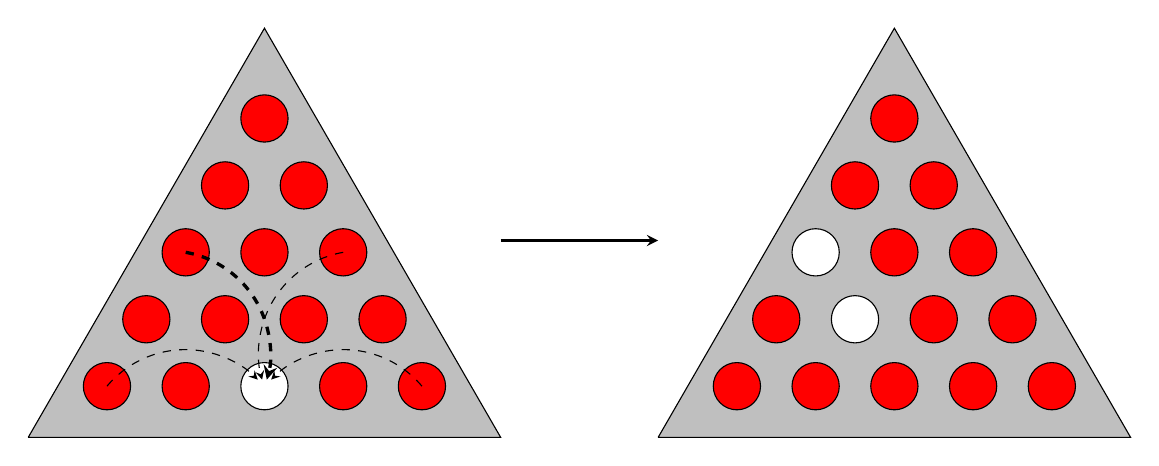
\begin{tikzpicture}[>=stealth]
\draw[fill=gray!50] (0,0) -- (3,5.196152423) -- (6,0)-- (0,0);




\draw[fill=red] (1,0.65) circle (0.3);
\draw[fill=red] (2,0.65) circle (0.3);
\draw[fill=white] (3,0.65) circle (0.3);
\draw[fill=red] (4,0.65) circle (0.3);
\draw[fill=red] (5,0.65) circle (0.3);

\draw[fill=red] (1.5,1.5) circle (0.3);
\draw[fill=red] (2.5,1.5) circle (0.3);
\draw[fill=red] (3.5,1.5) circle (0.3);
\draw[fill=red] (4.5,1.5) circle (0.3);

\draw[fill=red] (2,2.35) circle (0.3);
\draw[fill=red] (3,2.35) circle (0.3);
\draw[fill=red] (4,2.35) circle (0.3);

\draw[fill=red] (2.5,3.2) circle (0.3);
\draw[fill=red] (3.5,3.2) circle (0.3);

\draw[fill=red] (3,4.05) circle (0.3);

%\draw[dashed,thick,->] (1,0.65) -- (3,0.65);
%\draw[dashed,thick,->] (5,0.65) -- (3,0.65);
%\draw[dashed,thick,->] (2,2.35) -- (3,0.65);
%\draw[dashed,thick,->] (4,2.35) -- (3,0.65);


\draw [dashed,->] (1,0.65) arc (140:45:1.3cm);
\draw [dashed,->] (5,0.65) arc (40:135:1.3cm);
\draw [dashed,very thick,->] (2,2.35) arc (80:-15:1.3cm);
\draw [dashed,->] (4,2.35) arc (100:195:1.3cm);



\draw [thick,->] (6,2.5) -- (8,2.5);


\draw[fill=gray!50] (8,0) -- (11,5.196152423) -- (14,0)-- (8,0);




\draw[fill=red] (9,0.65) circle (0.3);
\draw[fill=red] (10,0.65) circle (0.3);
\draw[fill=red] (11,0.65) circle (0.3);
\draw[fill=red] (12,0.65) circle (0.3);
\draw[fill=red] (13,0.65) circle (0.3);

\draw[fill=red] (9.5,1.5) circle (0.3);
\draw[fill=white] (10.5,1.5) circle (0.3);
\draw[fill=red] (11.5,1.5) circle (0.3);
\draw[fill=red] (12.5,1.5) circle (0.3);

\draw[fill=white] (10,2.35) circle (0.3);
\draw[fill=red] (11,2.35) circle (0.3);
\draw[fill=red] (12,2.35) circle (0.3);

\draw[fill=red] (10.5,3.2) circle (0.3);
\draw[fill=red] (11.5,3.2) circle (0.3);

\draw[fill=red] (11,4.05) circle (0.3);

%\draw[dashed,thick,->] (1,0.65) -- (3,0.65);
%\draw[dashed,thick,->] (5,0.65) -- (3,0.65);
%\draw[dashed,thick,->] (2,2.35) -- (3,0.65);
%\draw[dashed,thick,->] (4,2.35) -- (3,0.65);


%\draw [dashed,->] (9,0.65) arc (140:45:1.3cm);
%\draw [dashed,->] (13,0.65) arc (40:135:1.3cm);
%\draw [dashed,very thick,->] (10,2.35) arc (80:-15:1.3cm);
%\draw [dashed,->] (12,2.35) arc (100:195:1.3cm);

\end{tikzpicture}

\end{center}
\caption{Initialized game field and possible transitions}
\label{fig:initGF}
\end{figure}

In this Figure we can see except initialization state also example of one
possible transition between two states. If it is target of the game to leave
only one position occupied with peg, it is obvious that we need $N - 1$ steps to
do that, where $N$ is count of positions in game field, because in every step we
lose one peg ($N = \frac{n(n-+1)}{2}$, where $n$ is length of side of the game
field, it is simple summmation of arithmetic progression). Now we should
declare, what we want to return from our program. Of course it will be sequence of states of game field, which lead to solution,
specifiyng occupation of concrete cell. Let us declare data structures, which
are necessary for computation.

First one will be definitely \textit{class Cell} containing boolean field
\verb|occupied| and maybe some information about its position in the game field
which is not very necessary for purpose of Squander computation. Next data
structure we need is \textit{class State} grouping individual cell together
defining actual state of game field. \textit{Class SolitaireSolver}, computing
configuration of states, has following fields:
\newpage
\begin{itemize}
  \item \textit{startState} defining inital state of the game field, where only
  one cell is not occupied
  \item \textit{integer n} for defining size of side of game field - it has to
  be greater or equal to 5
  \item \textit{integer array adj} containing type of adjacency (if exists)
  between cells, where index to that matrix is position of the cell in
  \verb|cells| array ($left=1, right=2, top_{45}=3, top_{135}=4, bottom_{135}=5,
  bottom_{45}=6$)
\end{itemize}

Now let us do the specification of the main method computing desirable sequence
of states. At first we will define some requirements on data structures we have.
We only allow to modify field \verb|occupied| of class \verb|Cell|, but only on
those instances, who are not representing \verb|startState|, because this state
has to be constant all the time (declared vis \verb|@Modifies| annotation and
optional instance selector in this annotation). Then we add constraint to object
\verb|startState|, that only one of the object in array \verb|Cells| can be
unoccupied. We declare this constraint using annotation \verb|@Invariant|
guarantees this constraint all the time (in this implementation will be enough
to use annotation \verb|@Required| when declaring this constraint, because we
allow to modify only \verb|Cell| objects in all states except for
\verb|startState|). Last requirement is that size of side of the triangle has
to be greater or equal to 5.

\lstinputlisting[label=ts1,caption=Defining requirements for Triangular
solitaire algorithm]{src/solitaire/TriSol1.java}

That were requirements for the algorithm. Now we have to add specifications
about the output of the algorithm. Specifications about returned array of states
are that all members of the result set are equal to all input states, because we
have to pass \uv{empty} states as method parameter. Last specification told us,
that only one cell of the last state is occupied. Specification is described in
Listing \ref{ts2}.
\newpage
\lstinputlisting[label=ts2,caption=Defining result set parameters for
Triangular solitaire algorithm]{src/solitaire/TriSol2.java}

Finally the most important thing is to add to method specification transition
constraints between two following states. In that constraint we specify that in
all states except last one exists three different cells such, that first one
(\verb|src|) and second one (\verb|via|) is occupied and the last one
(\verb|dest|) is empty and that value for first and second one and for the
second one and last one in the \verb|adj| matrix is the same and nonzero (that
means using positions of object cell in the \verb|cells| array of actual state
in \verb|adj| matrix to get type of adjacency if exists). If everything what was
mentioned is fulfilled, then is possible to make a transition such, that all
cell's occupied values are copied from actual state to following one except for
those three states mentioned above, which are copied inversively (\verb|src|,
\verb|via| and \verb|dest|) - see Listing \ref{ts3}.

This implementation works fine only for instances with up to 21 cells in game
field (side length 6). For larger instances was timeout treshold exceeded.
\newpage
\lstinputlisting[label=ts3,caption=Final implementation of
Triangular solitaire algorithm]{src/solitaire/TriSol3.java}


%*****************************************************************************
\chapter{Comparison}
For meausurement of some metrics (execution time and memory analysis) I have
tried to use Java profiler \textit{Test} \& \textit{Performance Tools Platform
(TPTP)}, which is Eclipse plugin profiling tool. This tool is highly integrated with Eclipse, so
it allows profiling of applications running from within Eclipse - see Figure
\ref{fig:pfMonitor}. This profiler had a big overhead when measuring Squnder
implementation and this led to situation, that every instance in Squander
reached time out. I have also tried another Eclipse profiler called
\textit{Colorer}, but developing of this profiler was cancelled in 2008 and also
there was quite a lot of problems to use it in oldest available Eclipse Europa.


\begin{figure}[ht]
\begin{center}
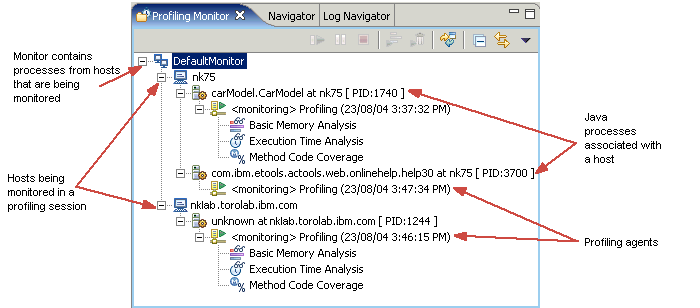
\includegraphics[width=14cm]{figures/pf}
\caption{TPTP profiling monitor}
\label{fig:pfMonitor}
\end{center}
\end{figure}

After that I decided to use tools provided by JVM, concretely \textit{JConsole}
(see Figure \ref{fig:pfJC}). This console can connect to any of running Java
process and monitore its Heap memory usage, CPU usage, number of load classes or
number of active threads. This data can be exported to csv file. It also
provides some statistics like CPU time, compile time, which kind of garbage
collector is used and how many collections were done etc.

For all measurement presented here, we had 1 warmup run and 5 test runs. The
purpose of the initial warmup run was to eliminate possible \uv{cold start}
effects, such as JVM initialization and class loading. In the subsequent 5 test runs, I executed
the operation under test on 3 same instances of a given
size, measured the total execution time, and reported the
average. The timeout threshold was set to 25 minutes for all experiments, and
the maximum Java heap size was left to the default value of 256MB. All
measurements were run a Linux box, with Intel\textsuperscript{\textregistered}
Core\texttrademark 2 Duo CPU @ 2.1GHz, 4GB of RAM, running Ubuntu 10.4.

\begin{figure}[ht]
\begin{center}
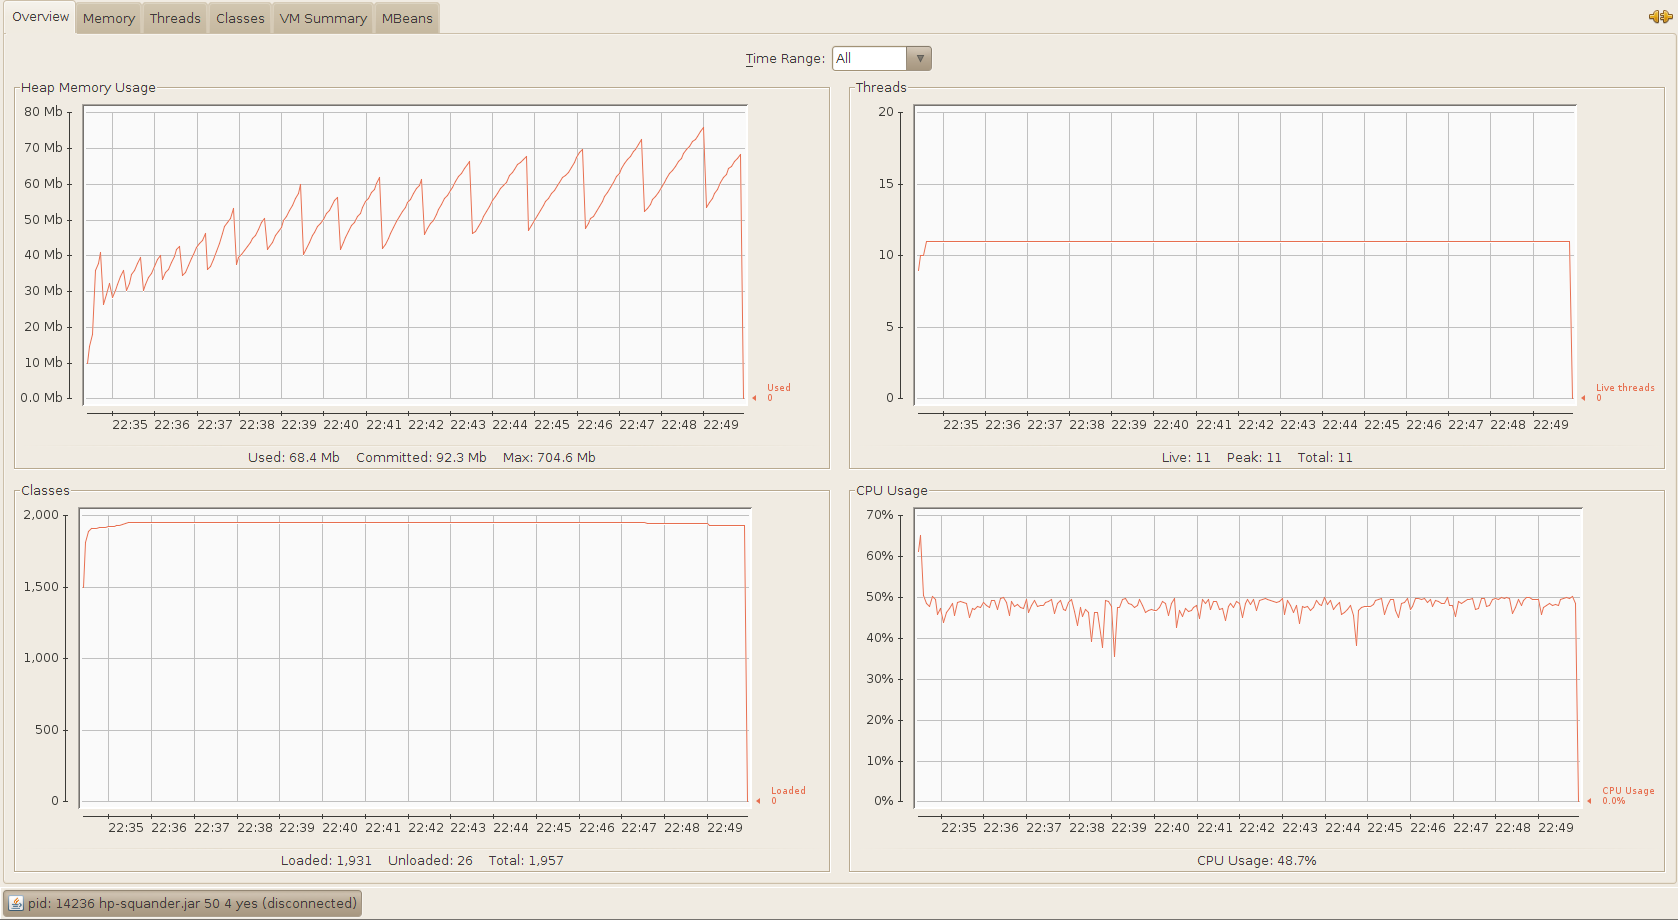
\includegraphics[width=14cm]{figures/jconsole/overview}
\caption{Profiling using JConsole}
\label{fig:pfJC}
\end{center}
\end{figure}


\subsection{Hamiltonian Path}

I used for measurement of implementation of algorithm Hamiltonian Path Squnder
implementation presented in \ref{sec:hp}. Impreative algorithm was implemented
as simple backtracking. In main method for finding solution is algorithm
iteratively going through matrix of followers row by row and when is resulted
array of edges (length of this array is number of nodes - 1) empty, the actual
egde is put at the beginning of the array. Another possibility is to put actual
edge into resulted array to concrete position when this condition is satisfied:
there is an edge between actual nodes in the iteration and in resulted array of
edge does not appear source node of this edge. Rule that source and destination
node af actual edge are different has to be fulfilled. After that if we are at
the end of resulted array, then we are return back from the recursion, otherwise
program is searching for the following edge in next recursive step. If program
is returned from recursive step in depth $n$ and none of the edges occupies
actual position in resulted array, then is edge from recursive step $n - 1$
removed, because following edge for edge in depth $n-1$ does not exist.
Implementation of algorithm with comments is in Listing \ref{hpImp}.


\lstinputlisting[label=hpImp,caption=Imperative
implementation of Hamiltonian Path algorithm]{src/hp/imp/GraphExecutor.java}

For testing both implementations I implemented simple graph generator
according to the rules mentioned in \ref{sec:gbb} and add restriction of maximal
grade of node in the graph. I made class \verb|Graph| serizalizable in order to
store it in some file and then load it into execution algorithm in order to run
both implementations on the same data.

In my test I have measured execution time of imperative backtrack method and
Squander implementation via method \verb|getCurrentThreadCpuTime()| of
\verb|ThreadMXBean| interface. According to \cite{oracle:javadoc}, a Java
virtual machine has a single instance of the implementation class of this interface. This instance implementing this
interface is an \verb|MXBean| that can be obtained by calling the
\verb|ManagementFactory.getThreadMXBean()| method or from the platform
\verb|MBeanServer| method. This method returns the total CPU time for the
current thread in nanoseconds. Results of the measurement are in Table
\ref{tab:hpTimes}.

From that table is obvious, that common imperative way of programming reached
better results than Squander implementation. In that point it is important to
note, that in execution time for Squander is included time for travesing heap,
checking preconditions and creating bounds for the universe, ensuring post
condition, translating to CNF and solving this CNF. We can also see, that bigger
influence on the execution time has maximal grade of node in the graph, mainly
in imperative implementation, because it causes branching during
backtracking.




\begin{table}[ht]
\caption{Execution times of Hamiltonian Path algorithm implementation in $\mu$s}
\label{tab:hpTimes}
\begin{center}
\begin{tabular}{l|l|l|l|l|l|l|l|l|l|} \cline{2-10}

\multirow{4}{*}{} & 
\multicolumn{9}{>{\cellcolor[gray]{.8}}c|}{Number of nodes
in the graph} \\ \cline{2-10} 
&  \multicolumn{4}{c|}{40} &
\multicolumn{2}{c|}{50} &
\multicolumn{3}{c|}{60}\\ \cline{2-10}
 & \multicolumn{4}{>{\cellcolor[gray]{.8}}c|}{max grade} &
\multicolumn{2}{>{\cellcolor[gray]{.8}}c|}{max grade} &
\multicolumn{3}{>{\cellcolor[gray]{.8}}c|}{max grade}\\ \cline{2-10}
 &  3 & 4 & 5 & 6 & 3 & 4 & 2 & 3 & 4  \\ \hline
\multicolumn{1}{|>{\cellcolor[gray]{.8}}l|}{Imperatively} & 180 &
4 220 & 39 910 & 772 860 & 120 & 60 390
& 10 & 440 & 780 \\ \hline
\multicolumn{1}{|>{\cellcolor[gray]{.8}}l|}{Squander} & 3 200 & 33 510 &
660 600 & \textbf{t/o} & 3 270 & 581 590 & 3 540 & 6 380 & \textbf{t/o}
\\
\hline
\end{tabular}
%\label{fig:hpIMem405}
\end{center}
\end{table}



\begin{table}
%\begin{center}
\begin{tabular}{l|l|l|l|l|l|l|l|l|l|} \cline{2-10}

\multirow{4}{*}{} & 
\multicolumn{9}{>{\cellcolor[gray]{.8}}c|}{Number of nodes
in the graph} \\ \cline{2-10} 

&  \multicolumn{3}{c|}{70} & \multicolumn{2}{c|}{80} &
 \multicolumn{2}{c|}{90} & \multicolumn{2}{c|}{100}\\ \cline{2-10}
 & \multicolumn{3}{>{\cellcolor[gray]{.8}}c|}{max grade} &
\multicolumn{2}{>{\cellcolor[gray]{.8}}c|}{max grade} &
\multicolumn{2}{>{\cellcolor[gray]{.8}}c|}{max grade} &
\multicolumn{2}{>{\cellcolor[gray]{.8}}c|}{max grade}\\ \cline{2-10}
&  2 & 3 & 4 & 2 & 3 & 2 & 3 & 2 & 3  \\ \hline
\multicolumn{1}{|>{\cellcolor[gray]{.8}}l|}{Imperatively}  & 30 & 3 940
& \textbf{t/o} & 20 & 14 920 & 70 & 173 090 & 40 &
 \textbf{t/o}\\ \hline 
\multicolumn{1}{|>{\cellcolor[gray]{.8}}l|}{Squander} & 3 940 & 5 100 &
\textbf{t/o} & 4 060 & 50 460 & 5 080 & \textbf{t/o} & 4 700 &
\textbf{t/o}\\ \hline
\end{tabular}

%\end{center}
\end{table}


\begin{figure}[ht]
\begin{center}
% GNUPLOT: LaTeX picture with Postscript
\begingroup
  \makeatletter
  \providecommand\color[2][]{%
    \GenericError{(gnuplot) \space\space\space\@spaces}{%
      Package color not loaded in conjunction with
      terminal option `colourtext'%
    }{See the gnuplot documentation for explanation.%
    }{Either use 'blacktext' in gnuplot or load the package
      color.sty in LaTeX.}%
    \renewcommand\color[2][]{}%
  }%
  \providecommand\includegraphics[2][]{%
    \GenericError{(gnuplot) \space\space\space\@spaces}{%
      Package graphicx or graphics not loaded%
    }{See the gnuplot documentation for explanation.%
    }{The gnuplot epslatex terminal needs graphicx.sty or graphics.sty.}%
    \renewcommand\includegraphics[2][]{}%
  }%
  \providecommand\rotatebox[2]{#2}%
  \@ifundefined{ifGPcolor}{%
    \newif\ifGPcolor
    \GPcolorfalse
  }{}%
  \@ifundefined{ifGPblacktext}{%
    \newif\ifGPblacktext
    \GPblacktexttrue
  }{}%
  % define a \g@addto@macro without @ in the name:
  \let\gplgaddtomacro\g@addto@macro
  % define empty templates for all commands taking text:
  \gdef\gplbacktext{}%
  \gdef\gplfronttext{}%
  \makeatother
  \ifGPblacktext
    % no textcolor at all
    \def\colorrgb#1{}%
    \def\colorgray#1{}%
  \else
    % gray or color?
    \ifGPcolor
      \def\colorrgb#1{\color[rgb]{#1}}%
      \def\colorgray#1{\color[gray]{#1}}%
      \expandafter\def\csname LTw\endcsname{\color{white}}%
      \expandafter\def\csname LTb\endcsname{\color{black}}%
      \expandafter\def\csname LTa\endcsname{\color{black}}%
      \expandafter\def\csname LT0\endcsname{\color[rgb]{1,0,0}}%
      \expandafter\def\csname LT1\endcsname{\color[rgb]{0,1,0}}%
      \expandafter\def\csname LT2\endcsname{\color[rgb]{0,0,1}}%
      \expandafter\def\csname LT3\endcsname{\color[rgb]{1,0,1}}%
      \expandafter\def\csname LT4\endcsname{\color[rgb]{0,1,1}}%
      \expandafter\def\csname LT5\endcsname{\color[rgb]{1,1,0}}%
      \expandafter\def\csname LT6\endcsname{\color[rgb]{0,0,0}}%
      \expandafter\def\csname LT7\endcsname{\color[rgb]{1,0.3,0}}%
      \expandafter\def\csname LT8\endcsname{\color[rgb]{0.5,0.5,0.5}}%
    \else
      % gray
      \def\colorrgb#1{\color{black}}%
      \def\colorgray#1{\color[gray]{#1}}%
      \expandafter\def\csname LTw\endcsname{\color{white}}%
      \expandafter\def\csname LTb\endcsname{\color{black}}%
      \expandafter\def\csname LTa\endcsname{\color{black}}%
      \expandafter\def\csname LT0\endcsname{\color{black}}%
      \expandafter\def\csname LT1\endcsname{\color{black}}%
      \expandafter\def\csname LT2\endcsname{\color{black}}%
      \expandafter\def\csname LT3\endcsname{\color{black}}%
      \expandafter\def\csname LT4\endcsname{\color{black}}%
      \expandafter\def\csname LT5\endcsname{\color{black}}%
      \expandafter\def\csname LT6\endcsname{\color{black}}%
      \expandafter\def\csname LT7\endcsname{\color{black}}%
      \expandafter\def\csname LT8\endcsname{\color{black}}%
    \fi
  \fi
  \setlength{\unitlength}{0.0500bp}%
  \begin{picture}(7200.00,5040.00)%
    \gplgaddtomacro\gplbacktext{%
      \csname LTb\endcsname%
      \put(1078,704){\makebox(0,0)[r]{\strut{} 0}}%
      \csname LTb\endcsname%
      \put(1078,1439){\makebox(0,0)[r]{\strut{} 5}}%
      \csname LTb\endcsname%
      \put(1078,2174){\makebox(0,0)[r]{\strut{} 10}}%
      \csname LTb\endcsname%
      \put(1078,2910){\makebox(0,0)[r]{\strut{} 15}}%
      \csname LTb\endcsname%
      \put(1078,3645){\makebox(0,0)[r]{\strut{} 20}}%
      \csname LTb\endcsname%
      \put(1078,4380){\makebox(0,0)[r]{\strut{} 25}}%
      \csname LTb\endcsname%
      \put(1210,484){\makebox(0,0){\strut{} 0}}%
      \csname LTb\endcsname%
      \put(1839,484){\makebox(0,0){\strut{} 10}}%
      \csname LTb\endcsname%
      \put(2468,484){\makebox(0,0){\strut{} 20}}%
      \csname LTb\endcsname%
      \put(3097,484){\makebox(0,0){\strut{} 30}}%
      \csname LTb\endcsname%
      \put(3726,484){\makebox(0,0){\strut{} 40}}%
      \csname LTb\endcsname%
      \put(4354,484){\makebox(0,0){\strut{} 50}}%
      \csname LTb\endcsname%
      \put(4983,484){\makebox(0,0){\strut{} 60}}%
      \csname LTb\endcsname%
      \put(5612,484){\makebox(0,0){\strut{} 70}}%
      \csname LTb\endcsname%
      \put(6241,484){\makebox(0,0){\strut{} 80}}%
      \csname LTb\endcsname%
      \put(6870,484){\makebox(0,0){\strut{} 90}}%
      \put(440,2542){\rotatebox{90}{\makebox(0,0){\strut{}used heap [Mb]}}}%
      \put(4040,154){\makebox(0,0){\strut{}time [s]}}%
      \put(4040,4710){\makebox(0,0){\strut{}Heap memory usage}}%
    }%
    \gplgaddtomacro\gplfronttext{%
    }%
    \gplbacktext
\put(0,0){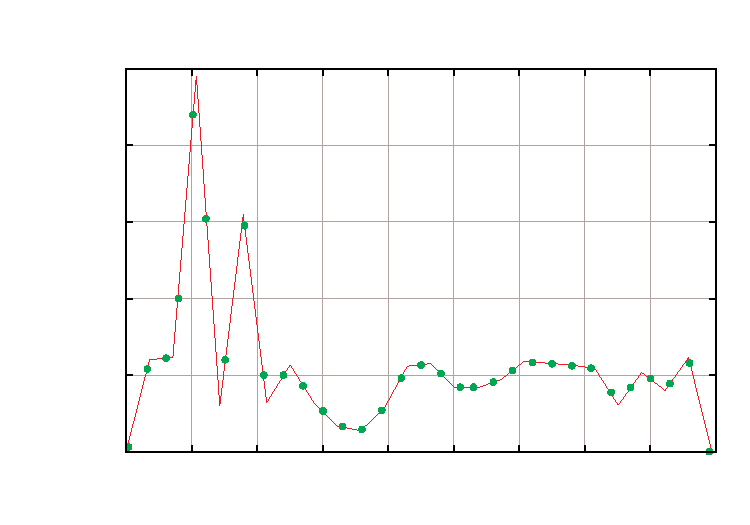
\includegraphics{figures/heap-ldsg-i-50-2-2}}%
    \gplfronttext
  \end{picture}%
\endgroup
\caption{Heap memory usage in time - Hamiltonian Path imperative algorithm for
graph of 40 nodes and maximal node grade 5}
\label{fig:hpIMem405}
\end{center}
\end{figure}


\begin{figure}[ht]
\begin{center}
% GNUPLOT: LaTeX picture with Postscript
\begingroup
  \makeatletter
  \providecommand\color[2][]{%
    \GenericError{(gnuplot) \space\space\space\@spaces}{%
      Package color not loaded in conjunction with
      terminal option `colourtext'%
    }{See the gnuplot documentation for explanation.%
    }{Either use 'blacktext' in gnuplot or load the package
      color.sty in LaTeX.}%
    \renewcommand\color[2][]{}%
  }%
  \providecommand\includegraphics[2][]{%
    \GenericError{(gnuplot) \space\space\space\@spaces}{%
      Package graphicx or graphics not loaded%
    }{See the gnuplot documentation for explanation.%
    }{The gnuplot epslatex terminal needs graphicx.sty or graphics.sty.}%
    \renewcommand\includegraphics[2][]{}%
  }%
  \providecommand\rotatebox[2]{#2}%
  \@ifundefined{ifGPcolor}{%
    \newif\ifGPcolor
    \GPcolorfalse
  }{}%
  \@ifundefined{ifGPblacktext}{%
    \newif\ifGPblacktext
    \GPblacktexttrue
  }{}%
  % define a \g@addto@macro without @ in the name:
  \let\gplgaddtomacro\g@addto@macro
  % define empty templates for all commands taking text:
  \gdef\gplbacktext{}%
  \gdef\gplfronttext{}%
  \makeatother
  \ifGPblacktext
    % no textcolor at all
    \def\colorrgb#1{}%
    \def\colorgray#1{}%
  \else
    % gray or color?
    \ifGPcolor
      \def\colorrgb#1{\color[rgb]{#1}}%
      \def\colorgray#1{\color[gray]{#1}}%
      \expandafter\def\csname LTw\endcsname{\color{white}}%
      \expandafter\def\csname LTb\endcsname{\color{black}}%
      \expandafter\def\csname LTa\endcsname{\color{black}}%
      \expandafter\def\csname LT0\endcsname{\color[rgb]{1,0,0}}%
      \expandafter\def\csname LT1\endcsname{\color[rgb]{0,1,0}}%
      \expandafter\def\csname LT2\endcsname{\color[rgb]{0,0,1}}%
      \expandafter\def\csname LT3\endcsname{\color[rgb]{1,0,1}}%
      \expandafter\def\csname LT4\endcsname{\color[rgb]{0,1,1}}%
      \expandafter\def\csname LT5\endcsname{\color[rgb]{1,1,0}}%
      \expandafter\def\csname LT6\endcsname{\color[rgb]{0,0,0}}%
      \expandafter\def\csname LT7\endcsname{\color[rgb]{1,0.3,0}}%
      \expandafter\def\csname LT8\endcsname{\color[rgb]{0.5,0.5,0.5}}%
    \else
      % gray
      \def\colorrgb#1{\color{black}}%
      \def\colorgray#1{\color[gray]{#1}}%
      \expandafter\def\csname LTw\endcsname{\color{white}}%
      \expandafter\def\csname LTb\endcsname{\color{black}}%
      \expandafter\def\csname LTa\endcsname{\color{black}}%
      \expandafter\def\csname LT0\endcsname{\color{black}}%
      \expandafter\def\csname LT1\endcsname{\color{black}}%
      \expandafter\def\csname LT2\endcsname{\color{black}}%
      \expandafter\def\csname LT3\endcsname{\color{black}}%
      \expandafter\def\csname LT4\endcsname{\color{black}}%
      \expandafter\def\csname LT5\endcsname{\color{black}}%
      \expandafter\def\csname LT6\endcsname{\color{black}}%
      \expandafter\def\csname LT7\endcsname{\color{black}}%
      \expandafter\def\csname LT8\endcsname{\color{black}}%
    \fi
  \fi
  \setlength{\unitlength}{0.0500bp}%
  \begin{picture}(7200.00,5040.00)%
    \gplgaddtomacro\gplbacktext{%
      \csname LTb\endcsname%
      \put(1078,704){\makebox(0,0)[r]{\strut{} 0}}%
      \csname LTb\endcsname%
      \put(1078,1229){\makebox(0,0)[r]{\strut{} 10}}%
      \csname LTb\endcsname%
      \put(1078,1754){\makebox(0,0)[r]{\strut{} 20}}%
      \csname LTb\endcsname%
      \put(1078,2279){\makebox(0,0)[r]{\strut{} 30}}%
      \csname LTb\endcsname%
      \put(1078,2805){\makebox(0,0)[r]{\strut{} 40}}%
      \csname LTb\endcsname%
      \put(1078,3330){\makebox(0,0)[r]{\strut{} 50}}%
      \csname LTb\endcsname%
      \put(1078,3855){\makebox(0,0)[r]{\strut{} 60}}%
      \csname LTb\endcsname%
      \put(1078,4380){\makebox(0,0)[r]{\strut{} 70}}%
      \csname LTb\endcsname%
      \put(1210,484){\makebox(0,0){\strut{} 0}}%
      \csname LTb\endcsname%
      \put(2019,484){\makebox(0,0){\strut{} 100}}%
      \csname LTb\endcsname%
      \put(2827,484){\makebox(0,0){\strut{} 200}}%
      \csname LTb\endcsname%
      \put(3636,484){\makebox(0,0){\strut{} 300}}%
      \csname LTb\endcsname%
      \put(4444,484){\makebox(0,0){\strut{} 400}}%
      \csname LTb\endcsname%
      \put(5253,484){\makebox(0,0){\strut{} 500}}%
      \csname LTb\endcsname%
      \put(6061,484){\makebox(0,0){\strut{} 600}}%
      \csname LTb\endcsname%
      \put(6870,484){\makebox(0,0){\strut{} 700}}%
      \put(440,2542){\rotatebox{90}{\makebox(0,0){\strut{}CPU used [\%]}}}%
      \put(4040,154){\makebox(0,0){\strut{}time [s]}}%
      \put(4040,4710){\makebox(0,0){\strut{}CPU usage}}%
    }%
    \gplgaddtomacro\gplfronttext{%
    }%
    \gplbacktext
    \put(0,0){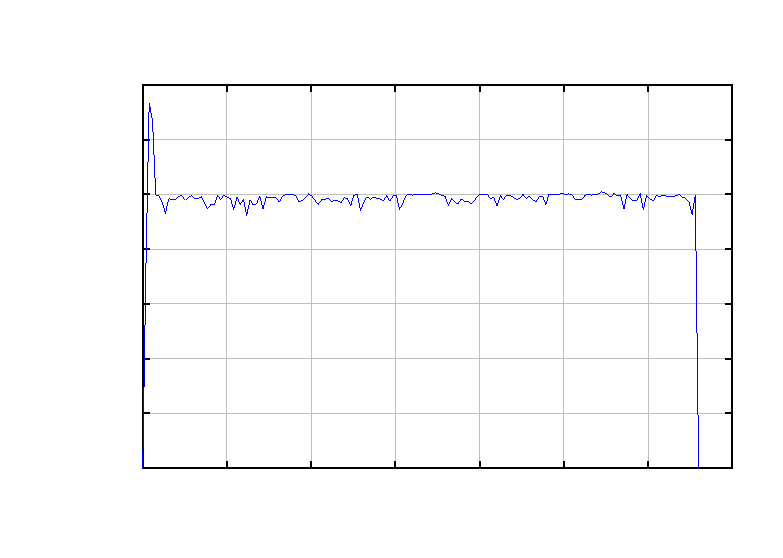
\includegraphics{figures/cpu-hp-s-40-5}}%
    \gplfronttext
  \end{picture}%
\endgroup
\caption{CPU usage in time - Hamiltonian Path imperative algorithm for graph
of 40 nodes and maximal node grade 5}
\label{fig:hpICpu405}
\end{center}
\end{figure}


\begin{figure}[ht]
\begin{center}
% GNUPLOT: LaTeX picture with Postscript
\begingroup
  \makeatletter
  \providecommand\color[2][]{%
    \GenericError{(gnuplot) \space\space\space\@spaces}{%
      Package color not loaded in conjunction with
      terminal option `colourtext'%
    }{See the gnuplot documentation for explanation.%
    }{Either use 'blacktext' in gnuplot or load the package
      color.sty in LaTeX.}%
    \renewcommand\color[2][]{}%
  }%
  \providecommand\includegraphics[2][]{%
    \GenericError{(gnuplot) \space\space\space\@spaces}{%
      Package graphicx or graphics not loaded%
    }{See the gnuplot documentation for explanation.%
    }{The gnuplot epslatex terminal needs graphicx.sty or graphics.sty.}%
    \renewcommand\includegraphics[2][]{}%
  }%
  \providecommand\rotatebox[2]{#2}%
  \@ifundefined{ifGPcolor}{%
    \newif\ifGPcolor
    \GPcolorfalse
  }{}%
  \@ifundefined{ifGPblacktext}{%
    \newif\ifGPblacktext
    \GPblacktexttrue
  }{}%
  % define a \g@addto@macro without @ in the name:
  \let\gplgaddtomacro\g@addto@macro
  % define empty templates for all commands taking text:
  \gdef\gplbacktext{}%
  \gdef\gplfronttext{}%
  \makeatother
  \ifGPblacktext
    % no textcolor at all
    \def\colorrgb#1{}%
    \def\colorgray#1{}%
  \else
    % gray or color?
    \ifGPcolor
      \def\colorrgb#1{\color[rgb]{#1}}%
      \def\colorgray#1{\color[gray]{#1}}%
      \expandafter\def\csname LTw\endcsname{\color{white}}%
      \expandafter\def\csname LTb\endcsname{\color{black}}%
      \expandafter\def\csname LTa\endcsname{\color{black}}%
      \expandafter\def\csname LT0\endcsname{\color[rgb]{1,0,0}}%
      \expandafter\def\csname LT1\endcsname{\color[rgb]{0,1,0}}%
      \expandafter\def\csname LT2\endcsname{\color[rgb]{0,0,1}}%
      \expandafter\def\csname LT3\endcsname{\color[rgb]{1,0,1}}%
      \expandafter\def\csname LT4\endcsname{\color[rgb]{0,1,1}}%
      \expandafter\def\csname LT5\endcsname{\color[rgb]{1,1,0}}%
      \expandafter\def\csname LT6\endcsname{\color[rgb]{0,0,0}}%
      \expandafter\def\csname LT7\endcsname{\color[rgb]{1,0.3,0}}%
      \expandafter\def\csname LT8\endcsname{\color[rgb]{0.5,0.5,0.5}}%
    \else
      % gray
      \def\colorrgb#1{\color{black}}%
      \def\colorgray#1{\color[gray]{#1}}%
      \expandafter\def\csname LTw\endcsname{\color{white}}%
      \expandafter\def\csname LTb\endcsname{\color{black}}%
      \expandafter\def\csname LTa\endcsname{\color{black}}%
      \expandafter\def\csname LT0\endcsname{\color{black}}%
      \expandafter\def\csname LT1\endcsname{\color{black}}%
      \expandafter\def\csname LT2\endcsname{\color{black}}%
      \expandafter\def\csname LT3\endcsname{\color{black}}%
      \expandafter\def\csname LT4\endcsname{\color{black}}%
      \expandafter\def\csname LT5\endcsname{\color{black}}%
      \expandafter\def\csname LT6\endcsname{\color{black}}%
      \expandafter\def\csname LT7\endcsname{\color{black}}%
      \expandafter\def\csname LT8\endcsname{\color{black}}%
    \fi
  \fi
  \setlength{\unitlength}{0.0500bp}%
  \begin{picture}(7200.00,5040.00)%
    \gplgaddtomacro\gplbacktext{%
      \csname LTb\endcsname%
      \put(1078,704){\makebox(0,0)[r]{\strut{} 0}}%
      \csname LTb\endcsname%
      \put(1078,1439){\makebox(0,0)[r]{\strut{} 5}}%
      \csname LTb\endcsname%
      \put(1078,2174){\makebox(0,0)[r]{\strut{} 10}}%
      \csname LTb\endcsname%
      \put(1078,2910){\makebox(0,0)[r]{\strut{} 15}}%
      \csname LTb\endcsname%
      \put(1078,3645){\makebox(0,0)[r]{\strut{} 20}}%
      \csname LTb\endcsname%
      \put(1078,4380){\makebox(0,0)[r]{\strut{} 25}}%
      \csname LTb\endcsname%
      \put(1210,484){\makebox(0,0){\strut{} 0}}%
      \csname LTb\endcsname%
      \put(1839,484){\makebox(0,0){\strut{} 10}}%
      \csname LTb\endcsname%
      \put(2468,484){\makebox(0,0){\strut{} 20}}%
      \csname LTb\endcsname%
      \put(3097,484){\makebox(0,0){\strut{} 30}}%
      \csname LTb\endcsname%
      \put(3726,484){\makebox(0,0){\strut{} 40}}%
      \csname LTb\endcsname%
      \put(4354,484){\makebox(0,0){\strut{} 50}}%
      \csname LTb\endcsname%
      \put(4983,484){\makebox(0,0){\strut{} 60}}%
      \csname LTb\endcsname%
      \put(5612,484){\makebox(0,0){\strut{} 70}}%
      \csname LTb\endcsname%
      \put(6241,484){\makebox(0,0){\strut{} 80}}%
      \csname LTb\endcsname%
      \put(6870,484){\makebox(0,0){\strut{} 90}}%
      \put(440,2542){\rotatebox{90}{\makebox(0,0){\strut{}used heap [Mb]}}}%
      \put(4040,154){\makebox(0,0){\strut{}time [s]}}%
      \put(4040,4710){\makebox(0,0){\strut{}Heap memory usage}}%
    }%
    \gplgaddtomacro\gplfronttext{%
    }%
    \gplbacktext
\put(0,0){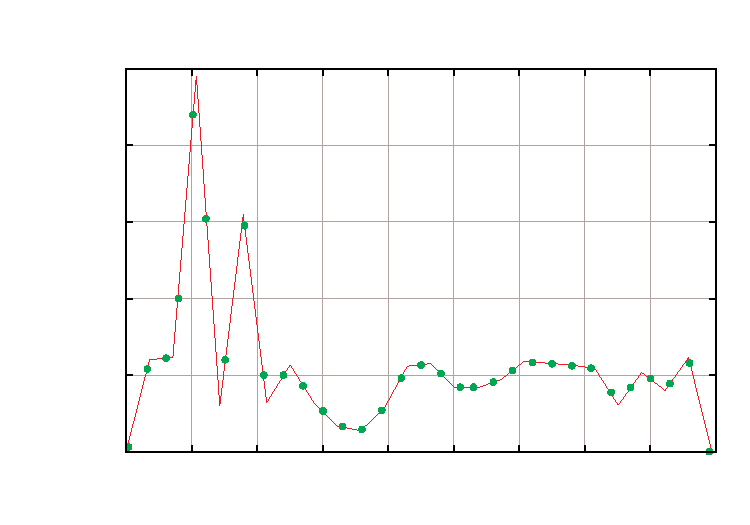
\includegraphics{figures/heap-ldsg-i-50-2-2}}%
    \gplfronttext
  \end{picture}%
\endgroup
\caption{Heap memory usage in time - Hamiltonian Path Squander algorithm for
graph of 40 nodes and maximal node grade 5}
\label{fig:hpSMem405}
\end{center}
\end{figure}



\begin{figure}[ht]
\begin{center}
% GNUPLOT: LaTeX picture with Postscript
\begingroup
  \makeatletter
  \providecommand\color[2][]{%
    \GenericError{(gnuplot) \space\space\space\@spaces}{%
      Package color not loaded in conjunction with
      terminal option `colourtext'%
    }{See the gnuplot documentation for explanation.%
    }{Either use 'blacktext' in gnuplot or load the package
      color.sty in LaTeX.}%
    \renewcommand\color[2][]{}%
  }%
  \providecommand\includegraphics[2][]{%
    \GenericError{(gnuplot) \space\space\space\@spaces}{%
      Package graphicx or graphics not loaded%
    }{See the gnuplot documentation for explanation.%
    }{The gnuplot epslatex terminal needs graphicx.sty or graphics.sty.}%
    \renewcommand\includegraphics[2][]{}%
  }%
  \providecommand\rotatebox[2]{#2}%
  \@ifundefined{ifGPcolor}{%
    \newif\ifGPcolor
    \GPcolorfalse
  }{}%
  \@ifundefined{ifGPblacktext}{%
    \newif\ifGPblacktext
    \GPblacktexttrue
  }{}%
  % define a \g@addto@macro without @ in the name:
  \let\gplgaddtomacro\g@addto@macro
  % define empty templates for all commands taking text:
  \gdef\gplbacktext{}%
  \gdef\gplfronttext{}%
  \makeatother
  \ifGPblacktext
    % no textcolor at all
    \def\colorrgb#1{}%
    \def\colorgray#1{}%
  \else
    % gray or color?
    \ifGPcolor
      \def\colorrgb#1{\color[rgb]{#1}}%
      \def\colorgray#1{\color[gray]{#1}}%
      \expandafter\def\csname LTw\endcsname{\color{white}}%
      \expandafter\def\csname LTb\endcsname{\color{black}}%
      \expandafter\def\csname LTa\endcsname{\color{black}}%
      \expandafter\def\csname LT0\endcsname{\color[rgb]{1,0,0}}%
      \expandafter\def\csname LT1\endcsname{\color[rgb]{0,1,0}}%
      \expandafter\def\csname LT2\endcsname{\color[rgb]{0,0,1}}%
      \expandafter\def\csname LT3\endcsname{\color[rgb]{1,0,1}}%
      \expandafter\def\csname LT4\endcsname{\color[rgb]{0,1,1}}%
      \expandafter\def\csname LT5\endcsname{\color[rgb]{1,1,0}}%
      \expandafter\def\csname LT6\endcsname{\color[rgb]{0,0,0}}%
      \expandafter\def\csname LT7\endcsname{\color[rgb]{1,0.3,0}}%
      \expandafter\def\csname LT8\endcsname{\color[rgb]{0.5,0.5,0.5}}%
    \else
      % gray
      \def\colorrgb#1{\color{black}}%
      \def\colorgray#1{\color[gray]{#1}}%
      \expandafter\def\csname LTw\endcsname{\color{white}}%
      \expandafter\def\csname LTb\endcsname{\color{black}}%
      \expandafter\def\csname LTa\endcsname{\color{black}}%
      \expandafter\def\csname LT0\endcsname{\color{black}}%
      \expandafter\def\csname LT1\endcsname{\color{black}}%
      \expandafter\def\csname LT2\endcsname{\color{black}}%
      \expandafter\def\csname LT3\endcsname{\color{black}}%
      \expandafter\def\csname LT4\endcsname{\color{black}}%
      \expandafter\def\csname LT5\endcsname{\color{black}}%
      \expandafter\def\csname LT6\endcsname{\color{black}}%
      \expandafter\def\csname LT7\endcsname{\color{black}}%
      \expandafter\def\csname LT8\endcsname{\color{black}}%
    \fi
  \fi
  \setlength{\unitlength}{0.0500bp}%
  \begin{picture}(7200.00,5040.00)%
    \gplgaddtomacro\gplbacktext{%
      \csname LTb\endcsname%
      \put(1078,704){\makebox(0,0)[r]{\strut{} 0}}%
      \csname LTb\endcsname%
      \put(1078,1229){\makebox(0,0)[r]{\strut{} 10}}%
      \csname LTb\endcsname%
      \put(1078,1754){\makebox(0,0)[r]{\strut{} 20}}%
      \csname LTb\endcsname%
      \put(1078,2279){\makebox(0,0)[r]{\strut{} 30}}%
      \csname LTb\endcsname%
      \put(1078,2805){\makebox(0,0)[r]{\strut{} 40}}%
      \csname LTb\endcsname%
      \put(1078,3330){\makebox(0,0)[r]{\strut{} 50}}%
      \csname LTb\endcsname%
      \put(1078,3855){\makebox(0,0)[r]{\strut{} 60}}%
      \csname LTb\endcsname%
      \put(1078,4380){\makebox(0,0)[r]{\strut{} 70}}%
      \csname LTb\endcsname%
      \put(1210,484){\makebox(0,0){\strut{} 0}}%
      \csname LTb\endcsname%
      \put(2019,484){\makebox(0,0){\strut{} 100}}%
      \csname LTb\endcsname%
      \put(2827,484){\makebox(0,0){\strut{} 200}}%
      \csname LTb\endcsname%
      \put(3636,484){\makebox(0,0){\strut{} 300}}%
      \csname LTb\endcsname%
      \put(4444,484){\makebox(0,0){\strut{} 400}}%
      \csname LTb\endcsname%
      \put(5253,484){\makebox(0,0){\strut{} 500}}%
      \csname LTb\endcsname%
      \put(6061,484){\makebox(0,0){\strut{} 600}}%
      \csname LTb\endcsname%
      \put(6870,484){\makebox(0,0){\strut{} 700}}%
      \put(440,2542){\rotatebox{90}{\makebox(0,0){\strut{}CPU used [\%]}}}%
      \put(4040,154){\makebox(0,0){\strut{}time [s]}}%
      \put(4040,4710){\makebox(0,0){\strut{}CPU usage}}%
    }%
    \gplgaddtomacro\gplfronttext{%
    }%
    \gplbacktext
    \put(0,0){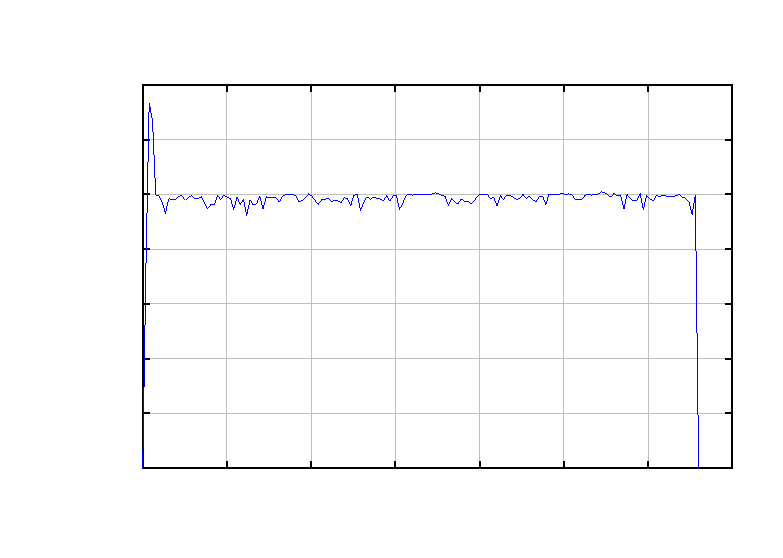
\includegraphics{figures/cpu-hp-s-40-5}}%
    \gplfronttext
  \end{picture}%
\endgroup
\caption{CPU usage in time - Hamiltonian Path Squander algorithm for graph
of 40 nodes and maximal node grade 5}
\label{fig:hpSCpu405}
\end{center}
\end{figure}



\begin{figure}[ht]
\begin{center}
% GNUPLOT: LaTeX picture with Postscript
\begingroup
  \makeatletter
  \providecommand\color[2][]{%
    \GenericError{(gnuplot) \space\space\space\@spaces}{%
      Package color not loaded in conjunction with
      terminal option `colourtext'%
    }{See the gnuplot documentation for explanation.%
    }{Either use 'blacktext' in gnuplot or load the package
      color.sty in LaTeX.}%
    \renewcommand\color[2][]{}%
  }%
  \providecommand\includegraphics[2][]{%
    \GenericError{(gnuplot) \space\space\space\@spaces}{%
      Package graphicx or graphics not loaded%
    }{See the gnuplot documentation for explanation.%
    }{The gnuplot epslatex terminal needs graphicx.sty or graphics.sty.}%
    \renewcommand\includegraphics[2][]{}%
  }%
  \providecommand\rotatebox[2]{#2}%
  \@ifundefined{ifGPcolor}{%
    \newif\ifGPcolor
    \GPcolorfalse
  }{}%
  \@ifundefined{ifGPblacktext}{%
    \newif\ifGPblacktext
    \GPblacktexttrue
  }{}%
  % define a \g@addto@macro without @ in the name:
  \let\gplgaddtomacro\g@addto@macro
  % define empty templates for all commands taking text:
  \gdef\gplbacktext{}%
  \gdef\gplfronttext{}%
  \makeatother
  \ifGPblacktext
    % no textcolor at all
    \def\colorrgb#1{}%
    \def\colorgray#1{}%
  \else
    % gray or color?
    \ifGPcolor
      \def\colorrgb#1{\color[rgb]{#1}}%
      \def\colorgray#1{\color[gray]{#1}}%
      \expandafter\def\csname LTw\endcsname{\color{white}}%
      \expandafter\def\csname LTb\endcsname{\color{black}}%
      \expandafter\def\csname LTa\endcsname{\color{black}}%
      \expandafter\def\csname LT0\endcsname{\color[rgb]{1,0,0}}%
      \expandafter\def\csname LT1\endcsname{\color[rgb]{0,1,0}}%
      \expandafter\def\csname LT2\endcsname{\color[rgb]{0,0,1}}%
      \expandafter\def\csname LT3\endcsname{\color[rgb]{1,0,1}}%
      \expandafter\def\csname LT4\endcsname{\color[rgb]{0,1,1}}%
      \expandafter\def\csname LT5\endcsname{\color[rgb]{1,1,0}}%
      \expandafter\def\csname LT6\endcsname{\color[rgb]{0,0,0}}%
      \expandafter\def\csname LT7\endcsname{\color[rgb]{1,0.3,0}}%
      \expandafter\def\csname LT8\endcsname{\color[rgb]{0.5,0.5,0.5}}%
    \else
      % gray
      \def\colorrgb#1{\color{black}}%
      \def\colorgray#1{\color[gray]{#1}}%
      \expandafter\def\csname LTw\endcsname{\color{white}}%
      \expandafter\def\csname LTb\endcsname{\color{black}}%
      \expandafter\def\csname LTa\endcsname{\color{black}}%
      \expandafter\def\csname LT0\endcsname{\color{black}}%
      \expandafter\def\csname LT1\endcsname{\color{black}}%
      \expandafter\def\csname LT2\endcsname{\color{black}}%
      \expandafter\def\csname LT3\endcsname{\color{black}}%
      \expandafter\def\csname LT4\endcsname{\color{black}}%
      \expandafter\def\csname LT5\endcsname{\color{black}}%
      \expandafter\def\csname LT6\endcsname{\color{black}}%
      \expandafter\def\csname LT7\endcsname{\color{black}}%
      \expandafter\def\csname LT8\endcsname{\color{black}}%
    \fi
  \fi
  \setlength{\unitlength}{0.0500bp}%
  \begin{picture}(7200.00,5040.00)%
    \gplgaddtomacro\gplbacktext{%
      \csname LTb\endcsname%
      \put(1078,704){\makebox(0,0)[r]{\strut{} 0}}%
      \csname LTb\endcsname%
      \put(1078,1439){\makebox(0,0)[r]{\strut{} 5}}%
      \csname LTb\endcsname%
      \put(1078,2174){\makebox(0,0)[r]{\strut{} 10}}%
      \csname LTb\endcsname%
      \put(1078,2910){\makebox(0,0)[r]{\strut{} 15}}%
      \csname LTb\endcsname%
      \put(1078,3645){\makebox(0,0)[r]{\strut{} 20}}%
      \csname LTb\endcsname%
      \put(1078,4380){\makebox(0,0)[r]{\strut{} 25}}%
      \csname LTb\endcsname%
      \put(1210,484){\makebox(0,0){\strut{} 0}}%
      \csname LTb\endcsname%
      \put(1839,484){\makebox(0,0){\strut{} 10}}%
      \csname LTb\endcsname%
      \put(2468,484){\makebox(0,0){\strut{} 20}}%
      \csname LTb\endcsname%
      \put(3097,484){\makebox(0,0){\strut{} 30}}%
      \csname LTb\endcsname%
      \put(3726,484){\makebox(0,0){\strut{} 40}}%
      \csname LTb\endcsname%
      \put(4354,484){\makebox(0,0){\strut{} 50}}%
      \csname LTb\endcsname%
      \put(4983,484){\makebox(0,0){\strut{} 60}}%
      \csname LTb\endcsname%
      \put(5612,484){\makebox(0,0){\strut{} 70}}%
      \csname LTb\endcsname%
      \put(6241,484){\makebox(0,0){\strut{} 80}}%
      \csname LTb\endcsname%
      \put(6870,484){\makebox(0,0){\strut{} 90}}%
      \put(440,2542){\rotatebox{90}{\makebox(0,0){\strut{}used heap [Mb]}}}%
      \put(4040,154){\makebox(0,0){\strut{}time [s]}}%
      \put(4040,4710){\makebox(0,0){\strut{}Heap memory usage}}%
    }%
    \gplgaddtomacro\gplfronttext{%
    }%
    \gplbacktext
\put(0,0){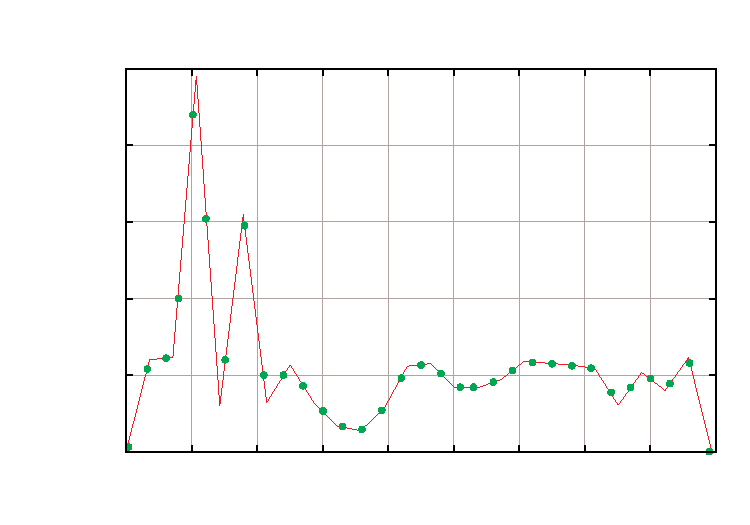
\includegraphics{figures/heap-ldsg-i-50-2-2}}%
    \gplfronttext
  \end{picture}%
\endgroup
\caption{Heap memory usage in time - Hamiltonian Path imperative algorithm for
graph of 50 nodes and maximal node grade 4}
\label{fig:hpIMem504}
\end{center}
\end{figure}

\begin{figure}[ht]
\begin{center}
% GNUPLOT: LaTeX picture with Postscript
\begingroup
  \makeatletter
  \providecommand\color[2][]{%
    \GenericError{(gnuplot) \space\space\space\@spaces}{%
      Package color not loaded in conjunction with
      terminal option `colourtext'%
    }{See the gnuplot documentation for explanation.%
    }{Either use 'blacktext' in gnuplot or load the package
      color.sty in LaTeX.}%
    \renewcommand\color[2][]{}%
  }%
  \providecommand\includegraphics[2][]{%
    \GenericError{(gnuplot) \space\space\space\@spaces}{%
      Package graphicx or graphics not loaded%
    }{See the gnuplot documentation for explanation.%
    }{The gnuplot epslatex terminal needs graphicx.sty or graphics.sty.}%
    \renewcommand\includegraphics[2][]{}%
  }%
  \providecommand\rotatebox[2]{#2}%
  \@ifundefined{ifGPcolor}{%
    \newif\ifGPcolor
    \GPcolorfalse
  }{}%
  \@ifundefined{ifGPblacktext}{%
    \newif\ifGPblacktext
    \GPblacktexttrue
  }{}%
  % define a \g@addto@macro without @ in the name:
  \let\gplgaddtomacro\g@addto@macro
  % define empty templates for all commands taking text:
  \gdef\gplbacktext{}%
  \gdef\gplfronttext{}%
  \makeatother
  \ifGPblacktext
    % no textcolor at all
    \def\colorrgb#1{}%
    \def\colorgray#1{}%
  \else
    % gray or color?
    \ifGPcolor
      \def\colorrgb#1{\color[rgb]{#1}}%
      \def\colorgray#1{\color[gray]{#1}}%
      \expandafter\def\csname LTw\endcsname{\color{white}}%
      \expandafter\def\csname LTb\endcsname{\color{black}}%
      \expandafter\def\csname LTa\endcsname{\color{black}}%
      \expandafter\def\csname LT0\endcsname{\color[rgb]{1,0,0}}%
      \expandafter\def\csname LT1\endcsname{\color[rgb]{0,1,0}}%
      \expandafter\def\csname LT2\endcsname{\color[rgb]{0,0,1}}%
      \expandafter\def\csname LT3\endcsname{\color[rgb]{1,0,1}}%
      \expandafter\def\csname LT4\endcsname{\color[rgb]{0,1,1}}%
      \expandafter\def\csname LT5\endcsname{\color[rgb]{1,1,0}}%
      \expandafter\def\csname LT6\endcsname{\color[rgb]{0,0,0}}%
      \expandafter\def\csname LT7\endcsname{\color[rgb]{1,0.3,0}}%
      \expandafter\def\csname LT8\endcsname{\color[rgb]{0.5,0.5,0.5}}%
    \else
      % gray
      \def\colorrgb#1{\color{black}}%
      \def\colorgray#1{\color[gray]{#1}}%
      \expandafter\def\csname LTw\endcsname{\color{white}}%
      \expandafter\def\csname LTb\endcsname{\color{black}}%
      \expandafter\def\csname LTa\endcsname{\color{black}}%
      \expandafter\def\csname LT0\endcsname{\color{black}}%
      \expandafter\def\csname LT1\endcsname{\color{black}}%
      \expandafter\def\csname LT2\endcsname{\color{black}}%
      \expandafter\def\csname LT3\endcsname{\color{black}}%
      \expandafter\def\csname LT4\endcsname{\color{black}}%
      \expandafter\def\csname LT5\endcsname{\color{black}}%
      \expandafter\def\csname LT6\endcsname{\color{black}}%
      \expandafter\def\csname LT7\endcsname{\color{black}}%
      \expandafter\def\csname LT8\endcsname{\color{black}}%
    \fi
  \fi
  \setlength{\unitlength}{0.0500bp}%
  \begin{picture}(7200.00,5040.00)%
    \gplgaddtomacro\gplbacktext{%
      \csname LTb\endcsname%
      \put(1078,704){\makebox(0,0)[r]{\strut{} 0}}%
      \csname LTb\endcsname%
      \put(1078,1229){\makebox(0,0)[r]{\strut{} 10}}%
      \csname LTb\endcsname%
      \put(1078,1754){\makebox(0,0)[r]{\strut{} 20}}%
      \csname LTb\endcsname%
      \put(1078,2279){\makebox(0,0)[r]{\strut{} 30}}%
      \csname LTb\endcsname%
      \put(1078,2805){\makebox(0,0)[r]{\strut{} 40}}%
      \csname LTb\endcsname%
      \put(1078,3330){\makebox(0,0)[r]{\strut{} 50}}%
      \csname LTb\endcsname%
      \put(1078,3855){\makebox(0,0)[r]{\strut{} 60}}%
      \csname LTb\endcsname%
      \put(1078,4380){\makebox(0,0)[r]{\strut{} 70}}%
      \csname LTb\endcsname%
      \put(1210,484){\makebox(0,0){\strut{} 0}}%
      \csname LTb\endcsname%
      \put(2019,484){\makebox(0,0){\strut{} 100}}%
      \csname LTb\endcsname%
      \put(2827,484){\makebox(0,0){\strut{} 200}}%
      \csname LTb\endcsname%
      \put(3636,484){\makebox(0,0){\strut{} 300}}%
      \csname LTb\endcsname%
      \put(4444,484){\makebox(0,0){\strut{} 400}}%
      \csname LTb\endcsname%
      \put(5253,484){\makebox(0,0){\strut{} 500}}%
      \csname LTb\endcsname%
      \put(6061,484){\makebox(0,0){\strut{} 600}}%
      \csname LTb\endcsname%
      \put(6870,484){\makebox(0,0){\strut{} 700}}%
      \put(440,2542){\rotatebox{90}{\makebox(0,0){\strut{}CPU used [\%]}}}%
      \put(4040,154){\makebox(0,0){\strut{}time [s]}}%
      \put(4040,4710){\makebox(0,0){\strut{}CPU usage}}%
    }%
    \gplgaddtomacro\gplfronttext{%
    }%
    \gplbacktext
    \put(0,0){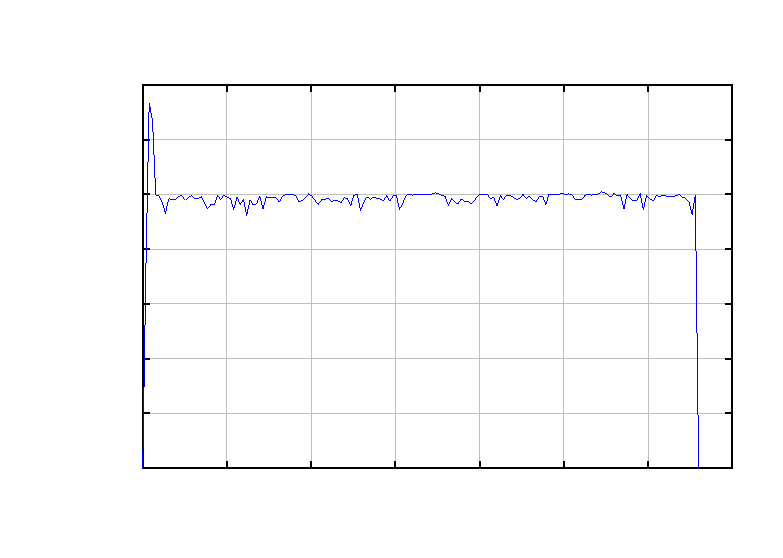
\includegraphics{figures/cpu-hp-s-40-5}}%
    \gplfronttext
  \end{picture}%
\endgroup
\caption{CPU usage in time - Hamiltonian Path imperative algorithm for graph
of 50 nodes and maximal node grade 4}
\label{fig:hpICpu504}
\end{center}
\end{figure}


\begin{figure}[ht]
\begin{center}
% GNUPLOT: LaTeX picture with Postscript
\begingroup
  \makeatletter
  \providecommand\color[2][]{%
    \GenericError{(gnuplot) \space\space\space\@spaces}{%
      Package color not loaded in conjunction with
      terminal option `colourtext'%
    }{See the gnuplot documentation for explanation.%
    }{Either use 'blacktext' in gnuplot or load the package
      color.sty in LaTeX.}%
    \renewcommand\color[2][]{}%
  }%
  \providecommand\includegraphics[2][]{%
    \GenericError{(gnuplot) \space\space\space\@spaces}{%
      Package graphicx or graphics not loaded%
    }{See the gnuplot documentation for explanation.%
    }{The gnuplot epslatex terminal needs graphicx.sty or graphics.sty.}%
    \renewcommand\includegraphics[2][]{}%
  }%
  \providecommand\rotatebox[2]{#2}%
  \@ifundefined{ifGPcolor}{%
    \newif\ifGPcolor
    \GPcolorfalse
  }{}%
  \@ifundefined{ifGPblacktext}{%
    \newif\ifGPblacktext
    \GPblacktexttrue
  }{}%
  % define a \g@addto@macro without @ in the name:
  \let\gplgaddtomacro\g@addto@macro
  % define empty templates for all commands taking text:
  \gdef\gplbacktext{}%
  \gdef\gplfronttext{}%
  \makeatother
  \ifGPblacktext
    % no textcolor at all
    \def\colorrgb#1{}%
    \def\colorgray#1{}%
  \else
    % gray or color?
    \ifGPcolor
      \def\colorrgb#1{\color[rgb]{#1}}%
      \def\colorgray#1{\color[gray]{#1}}%
      \expandafter\def\csname LTw\endcsname{\color{white}}%
      \expandafter\def\csname LTb\endcsname{\color{black}}%
      \expandafter\def\csname LTa\endcsname{\color{black}}%
      \expandafter\def\csname LT0\endcsname{\color[rgb]{1,0,0}}%
      \expandafter\def\csname LT1\endcsname{\color[rgb]{0,1,0}}%
      \expandafter\def\csname LT2\endcsname{\color[rgb]{0,0,1}}%
      \expandafter\def\csname LT3\endcsname{\color[rgb]{1,0,1}}%
      \expandafter\def\csname LT4\endcsname{\color[rgb]{0,1,1}}%
      \expandafter\def\csname LT5\endcsname{\color[rgb]{1,1,0}}%
      \expandafter\def\csname LT6\endcsname{\color[rgb]{0,0,0}}%
      \expandafter\def\csname LT7\endcsname{\color[rgb]{1,0.3,0}}%
      \expandafter\def\csname LT8\endcsname{\color[rgb]{0.5,0.5,0.5}}%
    \else
      % gray
      \def\colorrgb#1{\color{black}}%
      \def\colorgray#1{\color[gray]{#1}}%
      \expandafter\def\csname LTw\endcsname{\color{white}}%
      \expandafter\def\csname LTb\endcsname{\color{black}}%
      \expandafter\def\csname LTa\endcsname{\color{black}}%
      \expandafter\def\csname LT0\endcsname{\color{black}}%
      \expandafter\def\csname LT1\endcsname{\color{black}}%
      \expandafter\def\csname LT2\endcsname{\color{black}}%
      \expandafter\def\csname LT3\endcsname{\color{black}}%
      \expandafter\def\csname LT4\endcsname{\color{black}}%
      \expandafter\def\csname LT5\endcsname{\color{black}}%
      \expandafter\def\csname LT6\endcsname{\color{black}}%
      \expandafter\def\csname LT7\endcsname{\color{black}}%
      \expandafter\def\csname LT8\endcsname{\color{black}}%
    \fi
  \fi
  \setlength{\unitlength}{0.0500bp}%
  \begin{picture}(7200.00,5040.00)%
    \gplgaddtomacro\gplbacktext{%
      \csname LTb\endcsname%
      \put(1078,704){\makebox(0,0)[r]{\strut{} 0}}%
      \csname LTb\endcsname%
      \put(1078,1439){\makebox(0,0)[r]{\strut{} 5}}%
      \csname LTb\endcsname%
      \put(1078,2174){\makebox(0,0)[r]{\strut{} 10}}%
      \csname LTb\endcsname%
      \put(1078,2910){\makebox(0,0)[r]{\strut{} 15}}%
      \csname LTb\endcsname%
      \put(1078,3645){\makebox(0,0)[r]{\strut{} 20}}%
      \csname LTb\endcsname%
      \put(1078,4380){\makebox(0,0)[r]{\strut{} 25}}%
      \csname LTb\endcsname%
      \put(1210,484){\makebox(0,0){\strut{} 0}}%
      \csname LTb\endcsname%
      \put(1839,484){\makebox(0,0){\strut{} 10}}%
      \csname LTb\endcsname%
      \put(2468,484){\makebox(0,0){\strut{} 20}}%
      \csname LTb\endcsname%
      \put(3097,484){\makebox(0,0){\strut{} 30}}%
      \csname LTb\endcsname%
      \put(3726,484){\makebox(0,0){\strut{} 40}}%
      \csname LTb\endcsname%
      \put(4354,484){\makebox(0,0){\strut{} 50}}%
      \csname LTb\endcsname%
      \put(4983,484){\makebox(0,0){\strut{} 60}}%
      \csname LTb\endcsname%
      \put(5612,484){\makebox(0,0){\strut{} 70}}%
      \csname LTb\endcsname%
      \put(6241,484){\makebox(0,0){\strut{} 80}}%
      \csname LTb\endcsname%
      \put(6870,484){\makebox(0,0){\strut{} 90}}%
      \put(440,2542){\rotatebox{90}{\makebox(0,0){\strut{}used heap [Mb]}}}%
      \put(4040,154){\makebox(0,0){\strut{}time [s]}}%
      \put(4040,4710){\makebox(0,0){\strut{}Heap memory usage}}%
    }%
    \gplgaddtomacro\gplfronttext{%
    }%
    \gplbacktext
\put(0,0){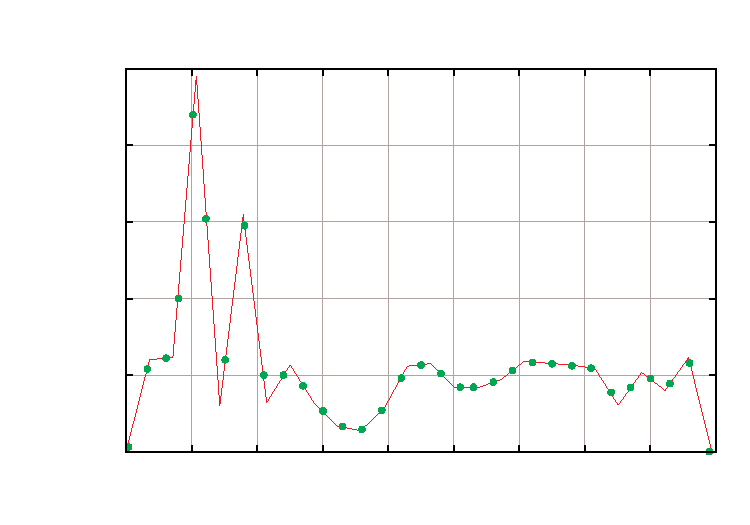
\includegraphics{figures/heap-ldsg-i-50-2-2}}%
    \gplfronttext
  \end{picture}%
\endgroup
\caption{Heap memory usage in time - Hamiltonian Path Sqaunder algorithm for
graph of 50 nodes and maximal node grade 4}
\label{fig:hpSMem504}
\end{center}
\end{figure}


\begin{figure}[ht]
\begin{center}
% GNUPLOT: LaTeX picture with Postscript
\begingroup
  \makeatletter
  \providecommand\color[2][]{%
    \GenericError{(gnuplot) \space\space\space\@spaces}{%
      Package color not loaded in conjunction with
      terminal option `colourtext'%
    }{See the gnuplot documentation for explanation.%
    }{Either use 'blacktext' in gnuplot or load the package
      color.sty in LaTeX.}%
    \renewcommand\color[2][]{}%
  }%
  \providecommand\includegraphics[2][]{%
    \GenericError{(gnuplot) \space\space\space\@spaces}{%
      Package graphicx or graphics not loaded%
    }{See the gnuplot documentation for explanation.%
    }{The gnuplot epslatex terminal needs graphicx.sty or graphics.sty.}%
    \renewcommand\includegraphics[2][]{}%
  }%
  \providecommand\rotatebox[2]{#2}%
  \@ifundefined{ifGPcolor}{%
    \newif\ifGPcolor
    \GPcolorfalse
  }{}%
  \@ifundefined{ifGPblacktext}{%
    \newif\ifGPblacktext
    \GPblacktexttrue
  }{}%
  % define a \g@addto@macro without @ in the name:
  \let\gplgaddtomacro\g@addto@macro
  % define empty templates for all commands taking text:
  \gdef\gplbacktext{}%
  \gdef\gplfronttext{}%
  \makeatother
  \ifGPblacktext
    % no textcolor at all
    \def\colorrgb#1{}%
    \def\colorgray#1{}%
  \else
    % gray or color?
    \ifGPcolor
      \def\colorrgb#1{\color[rgb]{#1}}%
      \def\colorgray#1{\color[gray]{#1}}%
      \expandafter\def\csname LTw\endcsname{\color{white}}%
      \expandafter\def\csname LTb\endcsname{\color{black}}%
      \expandafter\def\csname LTa\endcsname{\color{black}}%
      \expandafter\def\csname LT0\endcsname{\color[rgb]{1,0,0}}%
      \expandafter\def\csname LT1\endcsname{\color[rgb]{0,1,0}}%
      \expandafter\def\csname LT2\endcsname{\color[rgb]{0,0,1}}%
      \expandafter\def\csname LT3\endcsname{\color[rgb]{1,0,1}}%
      \expandafter\def\csname LT4\endcsname{\color[rgb]{0,1,1}}%
      \expandafter\def\csname LT5\endcsname{\color[rgb]{1,1,0}}%
      \expandafter\def\csname LT6\endcsname{\color[rgb]{0,0,0}}%
      \expandafter\def\csname LT7\endcsname{\color[rgb]{1,0.3,0}}%
      \expandafter\def\csname LT8\endcsname{\color[rgb]{0.5,0.5,0.5}}%
    \else
      % gray
      \def\colorrgb#1{\color{black}}%
      \def\colorgray#1{\color[gray]{#1}}%
      \expandafter\def\csname LTw\endcsname{\color{white}}%
      \expandafter\def\csname LTb\endcsname{\color{black}}%
      \expandafter\def\csname LTa\endcsname{\color{black}}%
      \expandafter\def\csname LT0\endcsname{\color{black}}%
      \expandafter\def\csname LT1\endcsname{\color{black}}%
      \expandafter\def\csname LT2\endcsname{\color{black}}%
      \expandafter\def\csname LT3\endcsname{\color{black}}%
      \expandafter\def\csname LT4\endcsname{\color{black}}%
      \expandafter\def\csname LT5\endcsname{\color{black}}%
      \expandafter\def\csname LT6\endcsname{\color{black}}%
      \expandafter\def\csname LT7\endcsname{\color{black}}%
      \expandafter\def\csname LT8\endcsname{\color{black}}%
    \fi
  \fi
  \setlength{\unitlength}{0.0500bp}%
  \begin{picture}(7200.00,5040.00)%
    \gplgaddtomacro\gplbacktext{%
      \csname LTb\endcsname%
      \put(1078,704){\makebox(0,0)[r]{\strut{} 0}}%
      \csname LTb\endcsname%
      \put(1078,1229){\makebox(0,0)[r]{\strut{} 10}}%
      \csname LTb\endcsname%
      \put(1078,1754){\makebox(0,0)[r]{\strut{} 20}}%
      \csname LTb\endcsname%
      \put(1078,2279){\makebox(0,0)[r]{\strut{} 30}}%
      \csname LTb\endcsname%
      \put(1078,2805){\makebox(0,0)[r]{\strut{} 40}}%
      \csname LTb\endcsname%
      \put(1078,3330){\makebox(0,0)[r]{\strut{} 50}}%
      \csname LTb\endcsname%
      \put(1078,3855){\makebox(0,0)[r]{\strut{} 60}}%
      \csname LTb\endcsname%
      \put(1078,4380){\makebox(0,0)[r]{\strut{} 70}}%
      \csname LTb\endcsname%
      \put(1210,484){\makebox(0,0){\strut{} 0}}%
      \csname LTb\endcsname%
      \put(2019,484){\makebox(0,0){\strut{} 100}}%
      \csname LTb\endcsname%
      \put(2827,484){\makebox(0,0){\strut{} 200}}%
      \csname LTb\endcsname%
      \put(3636,484){\makebox(0,0){\strut{} 300}}%
      \csname LTb\endcsname%
      \put(4444,484){\makebox(0,0){\strut{} 400}}%
      \csname LTb\endcsname%
      \put(5253,484){\makebox(0,0){\strut{} 500}}%
      \csname LTb\endcsname%
      \put(6061,484){\makebox(0,0){\strut{} 600}}%
      \csname LTb\endcsname%
      \put(6870,484){\makebox(0,0){\strut{} 700}}%
      \put(440,2542){\rotatebox{90}{\makebox(0,0){\strut{}CPU used [\%]}}}%
      \put(4040,154){\makebox(0,0){\strut{}time [s]}}%
      \put(4040,4710){\makebox(0,0){\strut{}CPU usage}}%
    }%
    \gplgaddtomacro\gplfronttext{%
    }%
    \gplbacktext
    \put(0,0){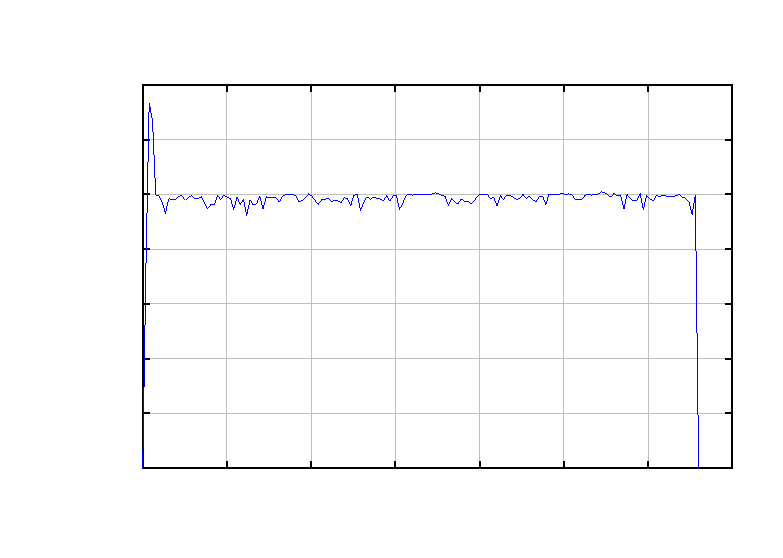
\includegraphics{figures/cpu-hp-s-40-5}}%
    \gplfronttext
  \end{picture}%
\endgroup
\caption{CPU usage in time - Hamiltonian Path Squander algorithm for graph
of 50 nodes and maximal node grade 4}
\label{fig:hpSCpu504}
\end{center}
\end{figure}


\begin{figure}[ht]
\begin{center}
% GNUPLOT: LaTeX picture with Postscript
\begingroup
  \makeatletter
  \providecommand\color[2][]{%
    \GenericError{(gnuplot) \space\space\space\@spaces}{%
      Package color not loaded in conjunction with
      terminal option `colourtext'%
    }{See the gnuplot documentation for explanation.%
    }{Either use 'blacktext' in gnuplot or load the package
      color.sty in LaTeX.}%
    \renewcommand\color[2][]{}%
  }%
  \providecommand\includegraphics[2][]{%
    \GenericError{(gnuplot) \space\space\space\@spaces}{%
      Package graphicx or graphics not loaded%
    }{See the gnuplot documentation for explanation.%
    }{The gnuplot epslatex terminal needs graphicx.sty or graphics.sty.}%
    \renewcommand\includegraphics[2][]{}%
  }%
  \providecommand\rotatebox[2]{#2}%
  \@ifundefined{ifGPcolor}{%
    \newif\ifGPcolor
    \GPcolorfalse
  }{}%
  \@ifundefined{ifGPblacktext}{%
    \newif\ifGPblacktext
    \GPblacktexttrue
  }{}%
  % define a \g@addto@macro without @ in the name:
  \let\gplgaddtomacro\g@addto@macro
  % define empty templates for all commands taking text:
  \gdef\gplbacktext{}%
  \gdef\gplfronttext{}%
  \makeatother
  \ifGPblacktext
    % no textcolor at all
    \def\colorrgb#1{}%
    \def\colorgray#1{}%
  \else
    % gray or color?
    \ifGPcolor
      \def\colorrgb#1{\color[rgb]{#1}}%
      \def\colorgray#1{\color[gray]{#1}}%
      \expandafter\def\csname LTw\endcsname{\color{white}}%
      \expandafter\def\csname LTb\endcsname{\color{black}}%
      \expandafter\def\csname LTa\endcsname{\color{black}}%
      \expandafter\def\csname LT0\endcsname{\color[rgb]{1,0,0}}%
      \expandafter\def\csname LT1\endcsname{\color[rgb]{0,1,0}}%
      \expandafter\def\csname LT2\endcsname{\color[rgb]{0,0,1}}%
      \expandafter\def\csname LT3\endcsname{\color[rgb]{1,0,1}}%
      \expandafter\def\csname LT4\endcsname{\color[rgb]{0,1,1}}%
      \expandafter\def\csname LT5\endcsname{\color[rgb]{1,1,0}}%
      \expandafter\def\csname LT6\endcsname{\color[rgb]{0,0,0}}%
      \expandafter\def\csname LT7\endcsname{\color[rgb]{1,0.3,0}}%
      \expandafter\def\csname LT8\endcsname{\color[rgb]{0.5,0.5,0.5}}%
    \else
      % gray
      \def\colorrgb#1{\color{black}}%
      \def\colorgray#1{\color[gray]{#1}}%
      \expandafter\def\csname LTw\endcsname{\color{white}}%
      \expandafter\def\csname LTb\endcsname{\color{black}}%
      \expandafter\def\csname LTa\endcsname{\color{black}}%
      \expandafter\def\csname LT0\endcsname{\color{black}}%
      \expandafter\def\csname LT1\endcsname{\color{black}}%
      \expandafter\def\csname LT2\endcsname{\color{black}}%
      \expandafter\def\csname LT3\endcsname{\color{black}}%
      \expandafter\def\csname LT4\endcsname{\color{black}}%
      \expandafter\def\csname LT5\endcsname{\color{black}}%
      \expandafter\def\csname LT6\endcsname{\color{black}}%
      \expandafter\def\csname LT7\endcsname{\color{black}}%
      \expandafter\def\csname LT8\endcsname{\color{black}}%
    \fi
  \fi
  \setlength{\unitlength}{0.0500bp}%
  \begin{picture}(7200.00,5040.00)%
    \gplgaddtomacro\gplbacktext{%
      \csname LTb\endcsname%
      \put(1078,704){\makebox(0,0)[r]{\strut{} 0}}%
      \csname LTb\endcsname%
      \put(1078,1439){\makebox(0,0)[r]{\strut{} 5}}%
      \csname LTb\endcsname%
      \put(1078,2174){\makebox(0,0)[r]{\strut{} 10}}%
      \csname LTb\endcsname%
      \put(1078,2910){\makebox(0,0)[r]{\strut{} 15}}%
      \csname LTb\endcsname%
      \put(1078,3645){\makebox(0,0)[r]{\strut{} 20}}%
      \csname LTb\endcsname%
      \put(1078,4380){\makebox(0,0)[r]{\strut{} 25}}%
      \csname LTb\endcsname%
      \put(1210,484){\makebox(0,0){\strut{} 0}}%
      \csname LTb\endcsname%
      \put(1839,484){\makebox(0,0){\strut{} 10}}%
      \csname LTb\endcsname%
      \put(2468,484){\makebox(0,0){\strut{} 20}}%
      \csname LTb\endcsname%
      \put(3097,484){\makebox(0,0){\strut{} 30}}%
      \csname LTb\endcsname%
      \put(3726,484){\makebox(0,0){\strut{} 40}}%
      \csname LTb\endcsname%
      \put(4354,484){\makebox(0,0){\strut{} 50}}%
      \csname LTb\endcsname%
      \put(4983,484){\makebox(0,0){\strut{} 60}}%
      \csname LTb\endcsname%
      \put(5612,484){\makebox(0,0){\strut{} 70}}%
      \csname LTb\endcsname%
      \put(6241,484){\makebox(0,0){\strut{} 80}}%
      \csname LTb\endcsname%
      \put(6870,484){\makebox(0,0){\strut{} 90}}%
      \put(440,2542){\rotatebox{90}{\makebox(0,0){\strut{}used heap [Mb]}}}%
      \put(4040,154){\makebox(0,0){\strut{}time [s]}}%
      \put(4040,4710){\makebox(0,0){\strut{}Heap memory usage}}%
    }%
    \gplgaddtomacro\gplfronttext{%
    }%
    \gplbacktext
\put(0,0){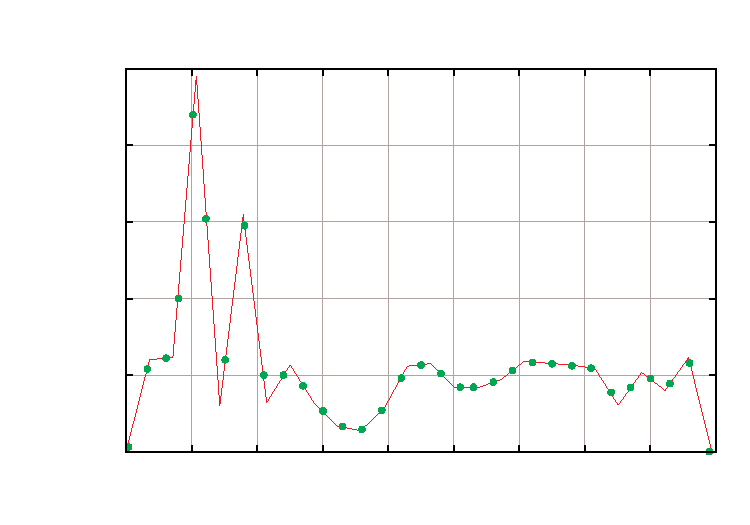
\includegraphics{figures/heap-ldsg-i-50-2-2}}%
    \gplfronttext
  \end{picture}%
\endgroup
\caption{Heap memory usage in time - Hamiltonian Path imperative algorithm for
graph of 80 nodes and maximal node grade 3}
\label{fig:hpIMem803}
\end{center}
\end{figure}

\begin{figure}[ht]
\begin{center}
% GNUPLOT: LaTeX picture with Postscript
\begingroup
  \makeatletter
  \providecommand\color[2][]{%
    \GenericError{(gnuplot) \space\space\space\@spaces}{%
      Package color not loaded in conjunction with
      terminal option `colourtext'%
    }{See the gnuplot documentation for explanation.%
    }{Either use 'blacktext' in gnuplot or load the package
      color.sty in LaTeX.}%
    \renewcommand\color[2][]{}%
  }%
  \providecommand\includegraphics[2][]{%
    \GenericError{(gnuplot) \space\space\space\@spaces}{%
      Package graphicx or graphics not loaded%
    }{See the gnuplot documentation for explanation.%
    }{The gnuplot epslatex terminal needs graphicx.sty or graphics.sty.}%
    \renewcommand\includegraphics[2][]{}%
  }%
  \providecommand\rotatebox[2]{#2}%
  \@ifundefined{ifGPcolor}{%
    \newif\ifGPcolor
    \GPcolorfalse
  }{}%
  \@ifundefined{ifGPblacktext}{%
    \newif\ifGPblacktext
    \GPblacktexttrue
  }{}%
  % define a \g@addto@macro without @ in the name:
  \let\gplgaddtomacro\g@addto@macro
  % define empty templates for all commands taking text:
  \gdef\gplbacktext{}%
  \gdef\gplfronttext{}%
  \makeatother
  \ifGPblacktext
    % no textcolor at all
    \def\colorrgb#1{}%
    \def\colorgray#1{}%
  \else
    % gray or color?
    \ifGPcolor
      \def\colorrgb#1{\color[rgb]{#1}}%
      \def\colorgray#1{\color[gray]{#1}}%
      \expandafter\def\csname LTw\endcsname{\color{white}}%
      \expandafter\def\csname LTb\endcsname{\color{black}}%
      \expandafter\def\csname LTa\endcsname{\color{black}}%
      \expandafter\def\csname LT0\endcsname{\color[rgb]{1,0,0}}%
      \expandafter\def\csname LT1\endcsname{\color[rgb]{0,1,0}}%
      \expandafter\def\csname LT2\endcsname{\color[rgb]{0,0,1}}%
      \expandafter\def\csname LT3\endcsname{\color[rgb]{1,0,1}}%
      \expandafter\def\csname LT4\endcsname{\color[rgb]{0,1,1}}%
      \expandafter\def\csname LT5\endcsname{\color[rgb]{1,1,0}}%
      \expandafter\def\csname LT6\endcsname{\color[rgb]{0,0,0}}%
      \expandafter\def\csname LT7\endcsname{\color[rgb]{1,0.3,0}}%
      \expandafter\def\csname LT8\endcsname{\color[rgb]{0.5,0.5,0.5}}%
    \else
      % gray
      \def\colorrgb#1{\color{black}}%
      \def\colorgray#1{\color[gray]{#1}}%
      \expandafter\def\csname LTw\endcsname{\color{white}}%
      \expandafter\def\csname LTb\endcsname{\color{black}}%
      \expandafter\def\csname LTa\endcsname{\color{black}}%
      \expandafter\def\csname LT0\endcsname{\color{black}}%
      \expandafter\def\csname LT1\endcsname{\color{black}}%
      \expandafter\def\csname LT2\endcsname{\color{black}}%
      \expandafter\def\csname LT3\endcsname{\color{black}}%
      \expandafter\def\csname LT4\endcsname{\color{black}}%
      \expandafter\def\csname LT5\endcsname{\color{black}}%
      \expandafter\def\csname LT6\endcsname{\color{black}}%
      \expandafter\def\csname LT7\endcsname{\color{black}}%
      \expandafter\def\csname LT8\endcsname{\color{black}}%
    \fi
  \fi
  \setlength{\unitlength}{0.0500bp}%
  \begin{picture}(7200.00,5040.00)%
    \gplgaddtomacro\gplbacktext{%
      \csname LTb\endcsname%
      \put(1078,704){\makebox(0,0)[r]{\strut{} 0}}%
      \csname LTb\endcsname%
      \put(1078,1229){\makebox(0,0)[r]{\strut{} 10}}%
      \csname LTb\endcsname%
      \put(1078,1754){\makebox(0,0)[r]{\strut{} 20}}%
      \csname LTb\endcsname%
      \put(1078,2279){\makebox(0,0)[r]{\strut{} 30}}%
      \csname LTb\endcsname%
      \put(1078,2805){\makebox(0,0)[r]{\strut{} 40}}%
      \csname LTb\endcsname%
      \put(1078,3330){\makebox(0,0)[r]{\strut{} 50}}%
      \csname LTb\endcsname%
      \put(1078,3855){\makebox(0,0)[r]{\strut{} 60}}%
      \csname LTb\endcsname%
      \put(1078,4380){\makebox(0,0)[r]{\strut{} 70}}%
      \csname LTb\endcsname%
      \put(1210,484){\makebox(0,0){\strut{} 0}}%
      \csname LTb\endcsname%
      \put(2019,484){\makebox(0,0){\strut{} 100}}%
      \csname LTb\endcsname%
      \put(2827,484){\makebox(0,0){\strut{} 200}}%
      \csname LTb\endcsname%
      \put(3636,484){\makebox(0,0){\strut{} 300}}%
      \csname LTb\endcsname%
      \put(4444,484){\makebox(0,0){\strut{} 400}}%
      \csname LTb\endcsname%
      \put(5253,484){\makebox(0,0){\strut{} 500}}%
      \csname LTb\endcsname%
      \put(6061,484){\makebox(0,0){\strut{} 600}}%
      \csname LTb\endcsname%
      \put(6870,484){\makebox(0,0){\strut{} 700}}%
      \put(440,2542){\rotatebox{90}{\makebox(0,0){\strut{}CPU used [\%]}}}%
      \put(4040,154){\makebox(0,0){\strut{}time [s]}}%
      \put(4040,4710){\makebox(0,0){\strut{}CPU usage}}%
    }%
    \gplgaddtomacro\gplfronttext{%
    }%
    \gplbacktext
    \put(0,0){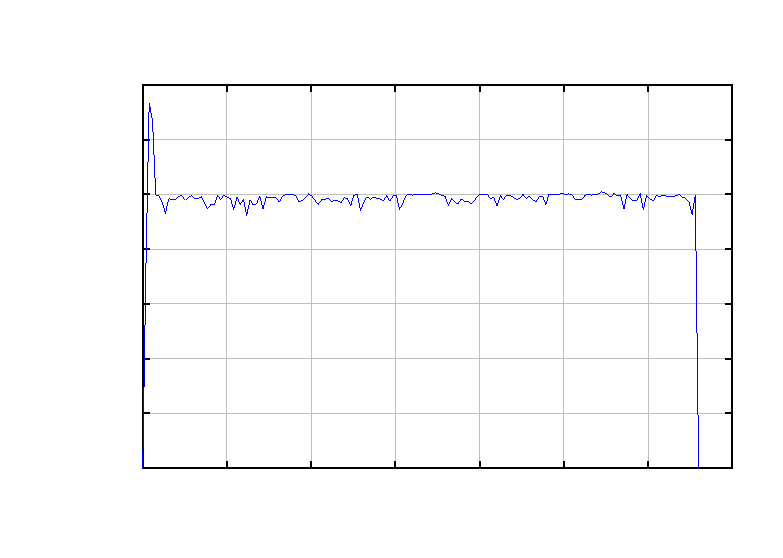
\includegraphics{figures/cpu-hp-s-40-5}}%
    \gplfronttext
  \end{picture}%
\endgroup
\caption{CPU usage in time - Hamiltonian Path imperative algorithm for graph
of 80 nodes and maximal node grade 3}
\label{fig:hpICpu803}
\end{center}
\end{figure}


\begin{figure}[ht]
\begin{center}
% GNUPLOT: LaTeX picture with Postscript
\begingroup
  \makeatletter
  \providecommand\color[2][]{%
    \GenericError{(gnuplot) \space\space\space\@spaces}{%
      Package color not loaded in conjunction with
      terminal option `colourtext'%
    }{See the gnuplot documentation for explanation.%
    }{Either use 'blacktext' in gnuplot or load the package
      color.sty in LaTeX.}%
    \renewcommand\color[2][]{}%
  }%
  \providecommand\includegraphics[2][]{%
    \GenericError{(gnuplot) \space\space\space\@spaces}{%
      Package graphicx or graphics not loaded%
    }{See the gnuplot documentation for explanation.%
    }{The gnuplot epslatex terminal needs graphicx.sty or graphics.sty.}%
    \renewcommand\includegraphics[2][]{}%
  }%
  \providecommand\rotatebox[2]{#2}%
  \@ifundefined{ifGPcolor}{%
    \newif\ifGPcolor
    \GPcolorfalse
  }{}%
  \@ifundefined{ifGPblacktext}{%
    \newif\ifGPblacktext
    \GPblacktexttrue
  }{}%
  % define a \g@addto@macro without @ in the name:
  \let\gplgaddtomacro\g@addto@macro
  % define empty templates for all commands taking text:
  \gdef\gplbacktext{}%
  \gdef\gplfronttext{}%
  \makeatother
  \ifGPblacktext
    % no textcolor at all
    \def\colorrgb#1{}%
    \def\colorgray#1{}%
  \else
    % gray or color?
    \ifGPcolor
      \def\colorrgb#1{\color[rgb]{#1}}%
      \def\colorgray#1{\color[gray]{#1}}%
      \expandafter\def\csname LTw\endcsname{\color{white}}%
      \expandafter\def\csname LTb\endcsname{\color{black}}%
      \expandafter\def\csname LTa\endcsname{\color{black}}%
      \expandafter\def\csname LT0\endcsname{\color[rgb]{1,0,0}}%
      \expandafter\def\csname LT1\endcsname{\color[rgb]{0,1,0}}%
      \expandafter\def\csname LT2\endcsname{\color[rgb]{0,0,1}}%
      \expandafter\def\csname LT3\endcsname{\color[rgb]{1,0,1}}%
      \expandafter\def\csname LT4\endcsname{\color[rgb]{0,1,1}}%
      \expandafter\def\csname LT5\endcsname{\color[rgb]{1,1,0}}%
      \expandafter\def\csname LT6\endcsname{\color[rgb]{0,0,0}}%
      \expandafter\def\csname LT7\endcsname{\color[rgb]{1,0.3,0}}%
      \expandafter\def\csname LT8\endcsname{\color[rgb]{0.5,0.5,0.5}}%
    \else
      % gray
      \def\colorrgb#1{\color{black}}%
      \def\colorgray#1{\color[gray]{#1}}%
      \expandafter\def\csname LTw\endcsname{\color{white}}%
      \expandafter\def\csname LTb\endcsname{\color{black}}%
      \expandafter\def\csname LTa\endcsname{\color{black}}%
      \expandafter\def\csname LT0\endcsname{\color{black}}%
      \expandafter\def\csname LT1\endcsname{\color{black}}%
      \expandafter\def\csname LT2\endcsname{\color{black}}%
      \expandafter\def\csname LT3\endcsname{\color{black}}%
      \expandafter\def\csname LT4\endcsname{\color{black}}%
      \expandafter\def\csname LT5\endcsname{\color{black}}%
      \expandafter\def\csname LT6\endcsname{\color{black}}%
      \expandafter\def\csname LT7\endcsname{\color{black}}%
      \expandafter\def\csname LT8\endcsname{\color{black}}%
    \fi
  \fi
  \setlength{\unitlength}{0.0500bp}%
  \begin{picture}(7200.00,5040.00)%
    \gplgaddtomacro\gplbacktext{%
      \csname LTb\endcsname%
      \put(1078,704){\makebox(0,0)[r]{\strut{} 0}}%
      \csname LTb\endcsname%
      \put(1078,1439){\makebox(0,0)[r]{\strut{} 5}}%
      \csname LTb\endcsname%
      \put(1078,2174){\makebox(0,0)[r]{\strut{} 10}}%
      \csname LTb\endcsname%
      \put(1078,2910){\makebox(0,0)[r]{\strut{} 15}}%
      \csname LTb\endcsname%
      \put(1078,3645){\makebox(0,0)[r]{\strut{} 20}}%
      \csname LTb\endcsname%
      \put(1078,4380){\makebox(0,0)[r]{\strut{} 25}}%
      \csname LTb\endcsname%
      \put(1210,484){\makebox(0,0){\strut{} 0}}%
      \csname LTb\endcsname%
      \put(1839,484){\makebox(0,0){\strut{} 10}}%
      \csname LTb\endcsname%
      \put(2468,484){\makebox(0,0){\strut{} 20}}%
      \csname LTb\endcsname%
      \put(3097,484){\makebox(0,0){\strut{} 30}}%
      \csname LTb\endcsname%
      \put(3726,484){\makebox(0,0){\strut{} 40}}%
      \csname LTb\endcsname%
      \put(4354,484){\makebox(0,0){\strut{} 50}}%
      \csname LTb\endcsname%
      \put(4983,484){\makebox(0,0){\strut{} 60}}%
      \csname LTb\endcsname%
      \put(5612,484){\makebox(0,0){\strut{} 70}}%
      \csname LTb\endcsname%
      \put(6241,484){\makebox(0,0){\strut{} 80}}%
      \csname LTb\endcsname%
      \put(6870,484){\makebox(0,0){\strut{} 90}}%
      \put(440,2542){\rotatebox{90}{\makebox(0,0){\strut{}used heap [Mb]}}}%
      \put(4040,154){\makebox(0,0){\strut{}time [s]}}%
      \put(4040,4710){\makebox(0,0){\strut{}Heap memory usage}}%
    }%
    \gplgaddtomacro\gplfronttext{%
    }%
    \gplbacktext
\put(0,0){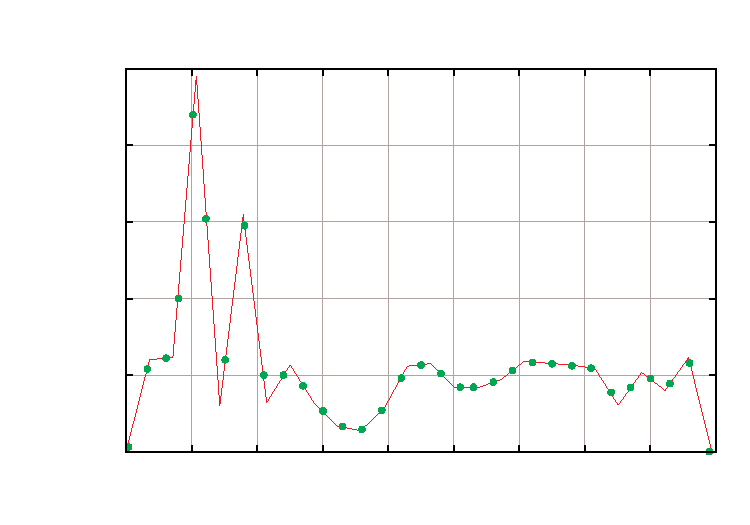
\includegraphics{figures/heap-ldsg-i-50-2-2}}%
    \gplfronttext
  \end{picture}%
\endgroup
\caption{Heap memory usage in time - Hamiltonian Path Sqaunder algorithm for
graph of 80 nodes and maximal node grade 3}
\label{fig:hpSMem803}
\end{center}
\end{figure}


\begin{figure}[ht]
\begin{center}
% GNUPLOT: LaTeX picture with Postscript
\begingroup
  \makeatletter
  \providecommand\color[2][]{%
    \GenericError{(gnuplot) \space\space\space\@spaces}{%
      Package color not loaded in conjunction with
      terminal option `colourtext'%
    }{See the gnuplot documentation for explanation.%
    }{Either use 'blacktext' in gnuplot or load the package
      color.sty in LaTeX.}%
    \renewcommand\color[2][]{}%
  }%
  \providecommand\includegraphics[2][]{%
    \GenericError{(gnuplot) \space\space\space\@spaces}{%
      Package graphicx or graphics not loaded%
    }{See the gnuplot documentation for explanation.%
    }{The gnuplot epslatex terminal needs graphicx.sty or graphics.sty.}%
    \renewcommand\includegraphics[2][]{}%
  }%
  \providecommand\rotatebox[2]{#2}%
  \@ifundefined{ifGPcolor}{%
    \newif\ifGPcolor
    \GPcolorfalse
  }{}%
  \@ifundefined{ifGPblacktext}{%
    \newif\ifGPblacktext
    \GPblacktexttrue
  }{}%
  % define a \g@addto@macro without @ in the name:
  \let\gplgaddtomacro\g@addto@macro
  % define empty templates for all commands taking text:
  \gdef\gplbacktext{}%
  \gdef\gplfronttext{}%
  \makeatother
  \ifGPblacktext
    % no textcolor at all
    \def\colorrgb#1{}%
    \def\colorgray#1{}%
  \else
    % gray or color?
    \ifGPcolor
      \def\colorrgb#1{\color[rgb]{#1}}%
      \def\colorgray#1{\color[gray]{#1}}%
      \expandafter\def\csname LTw\endcsname{\color{white}}%
      \expandafter\def\csname LTb\endcsname{\color{black}}%
      \expandafter\def\csname LTa\endcsname{\color{black}}%
      \expandafter\def\csname LT0\endcsname{\color[rgb]{1,0,0}}%
      \expandafter\def\csname LT1\endcsname{\color[rgb]{0,1,0}}%
      \expandafter\def\csname LT2\endcsname{\color[rgb]{0,0,1}}%
      \expandafter\def\csname LT3\endcsname{\color[rgb]{1,0,1}}%
      \expandafter\def\csname LT4\endcsname{\color[rgb]{0,1,1}}%
      \expandafter\def\csname LT5\endcsname{\color[rgb]{1,1,0}}%
      \expandafter\def\csname LT6\endcsname{\color[rgb]{0,0,0}}%
      \expandafter\def\csname LT7\endcsname{\color[rgb]{1,0.3,0}}%
      \expandafter\def\csname LT8\endcsname{\color[rgb]{0.5,0.5,0.5}}%
    \else
      % gray
      \def\colorrgb#1{\color{black}}%
      \def\colorgray#1{\color[gray]{#1}}%
      \expandafter\def\csname LTw\endcsname{\color{white}}%
      \expandafter\def\csname LTb\endcsname{\color{black}}%
      \expandafter\def\csname LTa\endcsname{\color{black}}%
      \expandafter\def\csname LT0\endcsname{\color{black}}%
      \expandafter\def\csname LT1\endcsname{\color{black}}%
      \expandafter\def\csname LT2\endcsname{\color{black}}%
      \expandafter\def\csname LT3\endcsname{\color{black}}%
      \expandafter\def\csname LT4\endcsname{\color{black}}%
      \expandafter\def\csname LT5\endcsname{\color{black}}%
      \expandafter\def\csname LT6\endcsname{\color{black}}%
      \expandafter\def\csname LT7\endcsname{\color{black}}%
      \expandafter\def\csname LT8\endcsname{\color{black}}%
    \fi
  \fi
  \setlength{\unitlength}{0.0500bp}%
  \begin{picture}(7200.00,5040.00)%
    \gplgaddtomacro\gplbacktext{%
      \csname LTb\endcsname%
      \put(1078,704){\makebox(0,0)[r]{\strut{} 0}}%
      \csname LTb\endcsname%
      \put(1078,1229){\makebox(0,0)[r]{\strut{} 10}}%
      \csname LTb\endcsname%
      \put(1078,1754){\makebox(0,0)[r]{\strut{} 20}}%
      \csname LTb\endcsname%
      \put(1078,2279){\makebox(0,0)[r]{\strut{} 30}}%
      \csname LTb\endcsname%
      \put(1078,2805){\makebox(0,0)[r]{\strut{} 40}}%
      \csname LTb\endcsname%
      \put(1078,3330){\makebox(0,0)[r]{\strut{} 50}}%
      \csname LTb\endcsname%
      \put(1078,3855){\makebox(0,0)[r]{\strut{} 60}}%
      \csname LTb\endcsname%
      \put(1078,4380){\makebox(0,0)[r]{\strut{} 70}}%
      \csname LTb\endcsname%
      \put(1210,484){\makebox(0,0){\strut{} 0}}%
      \csname LTb\endcsname%
      \put(2019,484){\makebox(0,0){\strut{} 100}}%
      \csname LTb\endcsname%
      \put(2827,484){\makebox(0,0){\strut{} 200}}%
      \csname LTb\endcsname%
      \put(3636,484){\makebox(0,0){\strut{} 300}}%
      \csname LTb\endcsname%
      \put(4444,484){\makebox(0,0){\strut{} 400}}%
      \csname LTb\endcsname%
      \put(5253,484){\makebox(0,0){\strut{} 500}}%
      \csname LTb\endcsname%
      \put(6061,484){\makebox(0,0){\strut{} 600}}%
      \csname LTb\endcsname%
      \put(6870,484){\makebox(0,0){\strut{} 700}}%
      \put(440,2542){\rotatebox{90}{\makebox(0,0){\strut{}CPU used [\%]}}}%
      \put(4040,154){\makebox(0,0){\strut{}time [s]}}%
      \put(4040,4710){\makebox(0,0){\strut{}CPU usage}}%
    }%
    \gplgaddtomacro\gplfronttext{%
    }%
    \gplbacktext
    \put(0,0){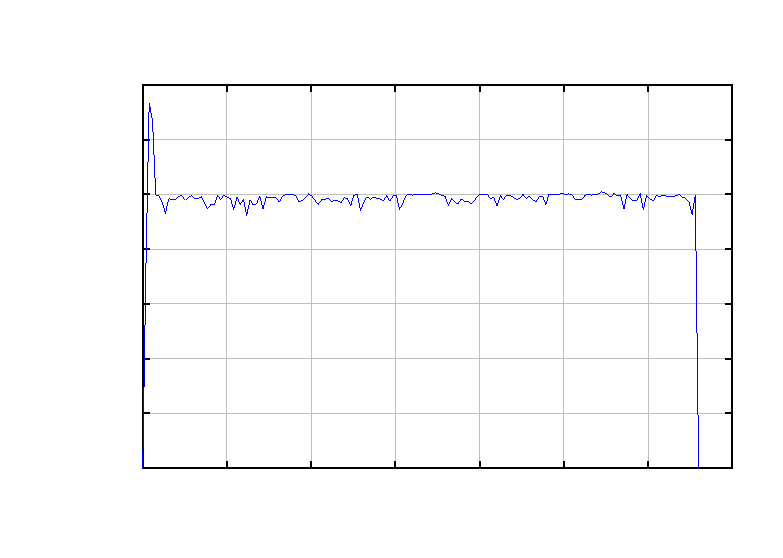
\includegraphics{figures/cpu-hp-s-40-5}}%
    \gplfronttext
  \end{picture}%
\endgroup
\caption{CPU usage in time - Hamiltonian Path Squander algorithm for graph
of 80 nodes and maximal node grade 3}
\label{fig:hpSCpu803}
\end{center}
\end{figure}

%*****************************************************************************
\chapter{Conclusion}

\begin{itemize}
\item Zhodnocení splnění cílů DP/BP a  vlastního přínosu práce (při formulaci je třeba vzít v potaz zadání práce).
\item Diskuse dalšího možného pokračování práce.
\end{itemize} 

%*****************************************************************************
% Seznam literatury je v samostatnem souboru reference.bib. Ten
% upravte dle vlastnich potreb, potom zpracujte (a do textu
% zapracujte) pomoci prikazu bibtex a nasledne pdflatex (nebo
% latex). Druhy z nich alespon 2x, aby se poresily odkazy.

\begin{thebibliography}{1}

\bibitem{milicevic:executableSpecificationsForJavaPrograms}
Aleksandar Milicevic; MASSACHUSETTS INSTITUTE OF TECHNOLOGY, Department of
Electrical Engineering and Computer Science; \textit{Executable Specifications
for Java Programs}, September 2010.

\bibitem{horstmannCornell:coreJava}
Cay Horstmann and Gary Cornell; \textit{Core Java}, 7th edition.

\bibitem{jirku:progProlog}
Petr Jirků a kol.; \textit{Programování v jazyku Prolog}, 1991.

\bibitem{kolar:jui}
doc. RNDr. Josef Kolář, CSc.; \textit{Jazyky pro umělou inteligenci}, 1994.

\bibitem{nino:pls}
Dr. Jaime Niño, Associate Professor of Computer Science; University of New
Orleans; \textit{Programming language structure - lectures}, 2011.

\bibitem{java:annotations}Annotations;\\
\verb|http://download.oracle.com/javase/1,5.0/docs/guide/language/annotations.html|

\bibitem{web:mathIsFun}Math
is fun
web;\\\verb|http://www.mathsisfun.com/games/triangle-peg-solitaire/index.html#|

\bibitem{oracle:javadoc}Oracle Java documentation;\\
\verb|http://download.oracle.com/javase/1,5,0/docs/api/|

\end{thebibliography}

% originally following specification for bibliography formating was used
%\bibliographystyle{abbrv}

% Here is an improvment by Petr Dlouhy (April 2010).
% It is mainly for supervisors who expect Czech fomrating rules for references
% Additional feature is live url addresses to sources from your pdf file
% It requires the file csplainnat.bst (included in this sample zipfile).

\bibliographystyle{csplainnat}

%bibliographystyle{plain}
%\bibliographystyle{psc}
{
%JZ: 11.12.2008 Kdo chce mit v techto ukazkovych odkazech take odkaz na CSTeX:
\def\CS{$\cal C\kern-0.1667em\lower.5ex\hbox{$\cal S$}\kern-0.075em $}
\bibliography{reference}
}


% M. Dušek radi:
%\bibliographystyle{alpha}
% kdy citace ma tvar [AutorRok] (napriklad [Cook97]). Sice to asi neni  podle ceske normy (BTW BibTeX stejne neodpovida ceske norme), ale je to nejprehlednejsi.
% 3.5.2009 JZ polemizuje: BibTeX neobvinujte, napiste a poskytnete nam styl (.bst) splnujici citacni normu CSN/ISO.

%*****************************************************************************
%*****************************************************************************
\appendix


%*****************************************************************************
\chapter{Pokyny a návody k formátování textu práce}
\textbf{\large Tato příloha samozřejmě nebude součástí vaší práce. Slouží pouze jako příklad formátování textu.}

Používat se dají všechny příkazy systému \LaTeX. Existuje velké množství volně přístupné dokumentace, tutoriálů, příruček a dalších materiálů v elektronické podobě. Výchozím bodem, kromě Googlu, může být stránka CSTUG (Czech Tech Users Group) \cite{CSTUG}. Tam najdete odkazy na další materiály.  Vetšinou dostačující a přehledně organizovanou elektronikou dokumentaci najdete například na \cite{latexdocweb} nebo \cite{latexwiki}.

Existují i různé nadstavby nad systémy \TeX{} a \LaTeX, které výrazně usnadní psaní textu zejména začátečníkům. Velmi rozšířený v Linuxovém prostředí je systém Kile.


\section{Vkládání obrázků}
Obrázky se umísťují do plovoucího prostředí \verb|figure|. Každý obrázek by měl obsahovat \textbf{název} (\verb|\caption|) a \textbf{návěští} (\verb|\label|). Použití příkazu pro vložení obrázku \\\verb|\includegraphics| je podmíněno aktivací (načtením) balíku graphicx příkazem\\ \verb|\usepackage{graphicx}|.

Budete-li zdrojový text zpracovávat pomocí programu \verb|pdflatex|, očekávají se obrázky s příponou \verb|*.pdf|\footnote{pdflatex umí také formáty PNG a JPG.}, použijete-li k formátování \verb|latex|, očekávají se obrázky s příponou \verb|*.eps|.\footnote{Vzájemnou konverzi mezi snad všemi typy obrazku včetně změn vekostí a dalších vymožeností vám může zajistit balík ImageMagic  (http://www.imagemagick.org/script/index.php). Je dostupný pod Linuxem, Mac OS i MS Windows. Důležité jsou zejména příkazy convert a identify.}

\begin{figure}[ht]
\begin{center}
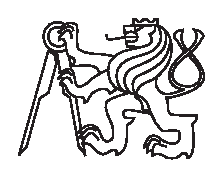
\includegraphics[width=5cm]{figures/LogoCVUT}
\caption{Popiska obrázku}
\label{fig:logo}
\end{center}
\end{figure}

Příklad vložení obrázku:
\begin{verbatim}
\begin{figure}[h]
\begin{center}
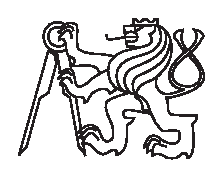
\includegraphics[width=5cm]{figures/LogoCVUT}
\caption{Popiska obrazku}
\label{fig:logo}
\end{center}
\end{figure}
\end{verbatim}

\section{Kreslení obrázků}
Zřejmě každý z vás má nějaký oblíbený nástroj pro tvorbu obrázků. Jde jen o to, abyste dokázali obrázek uložit v požadovaném formátu nebo jej do něj konvertovat (viz předchozí kapitola). Je zřejmě vhodné kreslit obrázky vektorově. Celkem oblíbený, na ovládání celkem jednoduchý a přitom dostatečně mocný je například program Inkscape.

Zde stojí za to upozornit na kreslící programe Ipe \cite{ipe}, který dokáže do obrázku vkládat komentáře přímo v latexovském formátu (vzroce, stejné fonty atd.). Podobné věci umí na Linuxové platformě nástroj Xfig. 

Za pozornost ještě stojí schopnost editoru Ipe importovat obrázek (jpg nebo bitmap) a krelit do něj latexovské popisky a komentáře. Výsledek pak umí exportovat přímo do pdf.

\section{Tabulky}
Existuje více způsobů, jak sázet tabulky. Například je možno použít prostředí \verb|table|, které je velmi podobné prostředí \verb|figure|. 

\begin{table}
\begin{center}
\begin{tabular}{|c|l|l|}
\hline
\textbf{DTD} & \textbf{construction} & \textbf{elimination} \\
\hline
$\mid$ & \verb+in1|A|B a:sum A B+ & \verb+case([_:A]a)([_:B]a)ab:A+\\
&\verb+in1|A|B b:sum A B+ & \verb+case([_:A]b)([_:B]b)ba:B+\\
\hline
$+$&\verb+do_reg:A -> reg A+&\verb+undo_reg:reg A -> A+\\
\hline
$*,?$& the same like $\mid$ and $+$ & the same like $\mid$ and $+$\\
& with \verb+emtpy_el:empty+ & with \verb+emtpy_el:empty+\\
\hline
R(a,b) & \verb+make_R:A->B->R+ & \verb+a: R -> A+\\
 & & \verb+b: R -> B+\\
\hline
\end{tabular}
\end{center}
\caption{Ukázka tabulky}
\label{tab:tab1}
\end{table}

Zdrojový text tabulky \ref{tab:tab1} vypadá takto:
\begin{verbatim}
\begin{table}
\begin{center}
\begin{tabular}{|c|l|l|}
\hline
\textbf{DTD} & \textbf{construction} & \textbf{elimination} \\
\hline
$\mid$ & \verb+in1|A|B a:sum A B+ & \verb+case([_:A]a)([_:B]a)ab:A+\\
&\verb+in1|A|B b:sum A B+ & \verb+case([_:A]b)([_:B]b)ba:B+\\
\hline
$+$&\verb+do_reg:A -> reg A+&\verb+undo_reg:reg A -> A+\\
\hline
$*,?$& the same like $\mid$ and $+$ & the same like $\mid$ and $+$\\
& with \verb+emtpy_el:empty+ & with \verb+emtpy_el:empty+\\
\hline
R(a,b) & \verb+make_R:A->B->R+ & \verb+a: R -> A+\\
 & & \verb+b: R -> B+\\
\hline
\end{tabular}
\end{center}
\caption{Ukázka tabulky}
\label{tab:tab1}
\end{table}
\begin{table}
\end{verbatim}

\section{Odkazy v textu}
\subsection{Odkazy na literaturu}
Jsou realizovány příkazem \verb|\cite{odkaz}|. 

Seznam literatury je dobré zapsat do samostatného souboru a ten pak zpracovat programem bibtex (viz soubor \verb|reference.bib|). Zdrojový soubor pro \verb|bibtex| vypadá například takto:
\begin{verbatim}
@Article{Chen01,
  author  = "Yong-Sheng Chen and Yi-Ping Hung and Chiou-Shann Fuh",
  title   = "Fast Block Matching Algorithm Based on 
             the Winner-Update Strategy",
  journal = "IEEE Transactions On Image Processing",
  pages   = "1212--1222",
  volume  =  10,
  number  =   8,
  year    = 2001,
}

@Misc{latexdocweb,
  author  = "",
  title   = "{\LaTeX} --- online manuál",
  note    = "\verb|http://www.cstug.cz/latex/lm/frames.html|",
  year    = "",
}
...
\end{verbatim}

%11.12.2008, 3.5.2009
\textbf{Pozor:} Sazba názvů odkazů je dána Bib\TeX{} stylem\\ (\verb|\bibliographystyle{abbrv}|). 
%Budete-li používat české prostředí (\verb|\usepackage[czech]{babel}|), 
Bib\TeX{} tedy obvykle vysází velké pouze počáteční písmeno z názvu zdroje, 
ostatní písmena zůstanou malá bez ohledu na to, jak je napíšete. 
Přesněji řečeno, styl může zvolit pro každý typ publikace jiné konverze. 
Pro časopisecké články třeba výše uvedené, jiné pro monografie (u nich často bývá 
naopak velikost písmen zachována).

Pokud chcete Bib\TeX u napovědět, která písmena nechat bez konverzí 
(viz \texttt{title = "\{$\backslash$LaTeX\} -{}-{}- online manuál"} 
v~předchozím příkladu), je nutné příslušné písmeno (zde celé makro) uzavřít 
do složených závorek. Pro přehlednost je proto vhodné celé parametry 
uzavírat do uvozovek (\texttt{author = "\dots"}), nikoliv do složených závorek.

Odkazy na literaturu ve zdrojovém textu se pak zapisují:
\begin{verbatim}
Podívejte se na \cite{Chen01}, 
další detaily najdete na \cite{latexdocweb}
\end{verbatim}

Vazbu mezi soubory \verb|*.tex| a \verb|*.bib| zajistíte příkazem 
\verb|\bibliography{}| v souboru \verb|*.tex|.  V našem případě tedy zdrojový 
dokument \verb|thesis.tex| obsahuje příkaz\\
\verb|\bibliography{reference}|.

Zpracování zdrojového textu s odkazy se provede postupným voláním programů\\
\verb|pdflatex <soubor>| (případně \verb|latex <soubor>|), \verb|bibtex <soubor>| 
a opět\\ \verb|pdflatex <soubor>|.\footnote{První volání \texttt{pdflatex} 
vytvoří soubor s~koncovkou \texttt{*.aux}, který je vstupem pro program 
\texttt{bibtex}, pak je potřeba znovu zavolat program \texttt{pdflatex} 
(\texttt{latex}), který tentokrát zpracuje soubory s příponami \texttt{.aux} a 
\texttt{.tex}. 
Informaci o případných nevyřešených odkazech (cross-reference) vidíte přímo při 
zpracovávání zdrojového souboru příkazem \texttt{pdflatex}. Program \texttt{pdflatex} 
(\texttt{latex}) lze volat vícekrát, pokud stále vidíte nevyřešené závislosti.}


Níže uvedený příklad je převzat z dříve existujících pokynů studentům, kteří 
dělají svou diplomovou nebo bakalářskou práci v~Grafické skupině.\footnote{Několikrát 
jsem byl upozorněn, že web s těmito pokyny byl zrušen, proto jej zde přímo necituji. 
Nicméně příklad sám o sobě dokumentuje obecně přijímaný konsensus ohledně citací 
v~bakalářských a diplomových pracích na KP.} Zde se praví:
\begin{small}
\begin{verbatim}
...
j) Seznam literatury a dalších použitých pramenů, odkazy na WWW stránky, ...
 Pozor na to, že na veškeré uvedené prameny se musíte v textu práce 
 odkazovat -- [1]. 
Pramen, na který neodkazujete, vypadá, že jste ho vlastně nepotřebovali 
a je uveden jen do počtu. Příklad citace knihy [1], článku v časopise [2], 
stati ve sborníku [3] a html odkazu [4]: 
[1] J. Žára, B. Beneš;, and P. Felkel. 
     Moderní počítačová grafika. Computer Press s.r.o, Brno, 1 edition, 1998. 
     (in Czech). 
[2] P. Slavík. Grammars and Rewriting Systems as Models for Graphical User 
     Interfaces. Cognitive Systems, 4(4--3):381--399, 1997. 
[3] M. Haindl, Š. Kment, and P. Slavík. Virtual Information Systems. 
     In WSCG'2000 -- Short communication papers, pages 22--27, Pilsen, 2000. 
     University of West Bohemia. 
[4] Knihovna grafické skupiny katedry počítačů: 
     http://www.cgg.cvut.cz/Bib/library/ 
\end{verbatim}
\end{small}
\ldots{} abychom výše citované odkazy skutečně našli v (automaticky generovaném) seznamu literatury tohoto textu, musíme je nyní alespoň jednou citovat: Kniha \cite{kniha}, článek v~časopisu \cite{clanek}, příspěvek na konferenci \cite{sbornik}, www odkaz \cite{www}.

Ještě přidáme další ukázku citací online zdrojů podle české normy. Odkaz na wiki o frameworcich \cite{wiki:framework} a ORM \cite{wiki:orm}. Použití viz soubor \verb|reference.bib|. V seznamu literatury by nyní měly být živé odkazy na zdroje. V \verb|reference.bib| je zcela nový typ publikace. Detaily dohledal a dodal Petr Dlouhý v dubnu 2010. Podrobnosti najdete ve zdrojovém souboru tohoto textu v komentáři u příkazu \verb|\thebibliography|.

\subsection{Odkazy na obrázky, tabulky a kapitoly}
\begin{itemize}
\item Označení místa v textu, na které chcete později čtenáře práce odkázat, se provede příkazem \verb|\label{navesti}|. Lze použít v prostředích \verb|figure| a  \verb|table|, ale též za názvem kapitoly nebo podkapitoly.
\item Na návěští se odkážeme příkazem \verb|\ref{navesti}| nebo \verb|\pageref{navesti}|.
\end{itemize}

\section{Rovnice, centrovaná, číslovaná matematika}
Jednoduchý matematický výraz zapsaný přímo do textu se vysází pomocí prostředí \verb|math|, resp. zkrácený zápis pomocí uzavření textu rovnice mezi znaky \verb|$|.

Kód \verb|$ S = \pi * r^2 $| bude vysázen takto: $ S = \pi * r^2 $.

Pokud chcete nečíslované rovnice, ale umístěné centrovaně na samostatné řádky, pak lze použít prostředí \verb|displaymath|, resp. zkrácený zápis pomocí uzavření textu rovnice mezi znaky \verb|$$|. Zdrojový kód: 
\begin{verb}
|$$ S = \pi * r^2 $$|
\end{verb}
bude pak vysázen takto:
$$ S = \pi * r^2 $$

Chcete-li mít rovnice číslované, je třeba použít prostředí \verb|eqation|. Kód:
\begin{verbatim}
\begin{equation}
  S = \pi * r^2
\end{equation}

\begin{equation}
  V = \pi * r^3
\end{equation}
\end{verbatim}
je potom vysázen takto:
\begin{equation}
  S = \pi * r^2
\end{equation}

\begin{equation}
  V = \pi * r^3
\end{equation}

\section{Kódy programu}
Chceme-li vysázet například část zdrojového kódu programu (bez formátování), hodí se prostředí \verb|verbatim|: 
\begin{verbatim}
         (* nickname2 *)
Lego> Refine in1
             (do_reg (nickname1 h));
Refine by  in1 (do_reg (nickname1 h))
   ?4 : pcdata
   ?5 : pcdata
          (* surname2 *)
Lego> Refine surname1 h;
Refine by  surname1 h
   ?5 : pcdata
          (* email2 *)
Lego> Refine undo_reg (email1 h);
Refine by  undo_reg (email1 h)
*** QED ***
\end{verbatim}

\section{Další poznámky}
\subsection{České uvozovky}
V souboru \verb|k336_thesis_macros.tex| je příkaz \verb|\uv{}| pro sázení českých uvozovek. \uv{Text uzavřený do českých uvozovek.}

% JZ: 3.5.2009 \chapter z book zajistí automaticky
%\subsection{Začátky kapitol na liché stránky}
%Ve výsledném textu je dobré, když každá kapitola začíná na liché stránce. Tedy použijte:
%\begin{verbatim}
%  \cleardoublepage\include{1_uvod}
%  \cleardoublepage\include{2_teorie}
%   atd.\ldots{}
%\end{verbatim}

%*****************************************************************************
\chapter{Seznam použitých zkratek}

\begin{description}
\item[2D] Two-Dimensional
\item[ABN] Abstract Boolean Networks
\item[ASIC] Application-Specific Integrated Circuit
\end{description}
\vdots

%*****************************************************************************
\chapter{UML diagramy}
\textbf{\large Tato příloha není povinná a zřejmě se neobjeví v každé práci. Máte-li ale větší množství podobných diagramů popisujících systém, není nutné všechny umísťovat do hlavního textu, zvláště pokud by to snižovalo jeho čitelnost.}

%*****************************************************************************
\chapter{Instalační a uživatelská příručka}
\textbf{\large Tato příloha velmi žádoucí zejména u softwarových implementačních prací.}

%*****************************************************************************
\chapter{Obsah přiloženého CD}
\textbf{\large Tato příloha je povinná pro každou práci. Každá práce musí totiž obsahovat přiložené CD. Viz dále.}

Může vypadat například takto. Váš seznam samozřejmě bude odpovídat typu vaší práce. (viz \cite{infodp}):

\begin{figure}[h]
\begin{center}
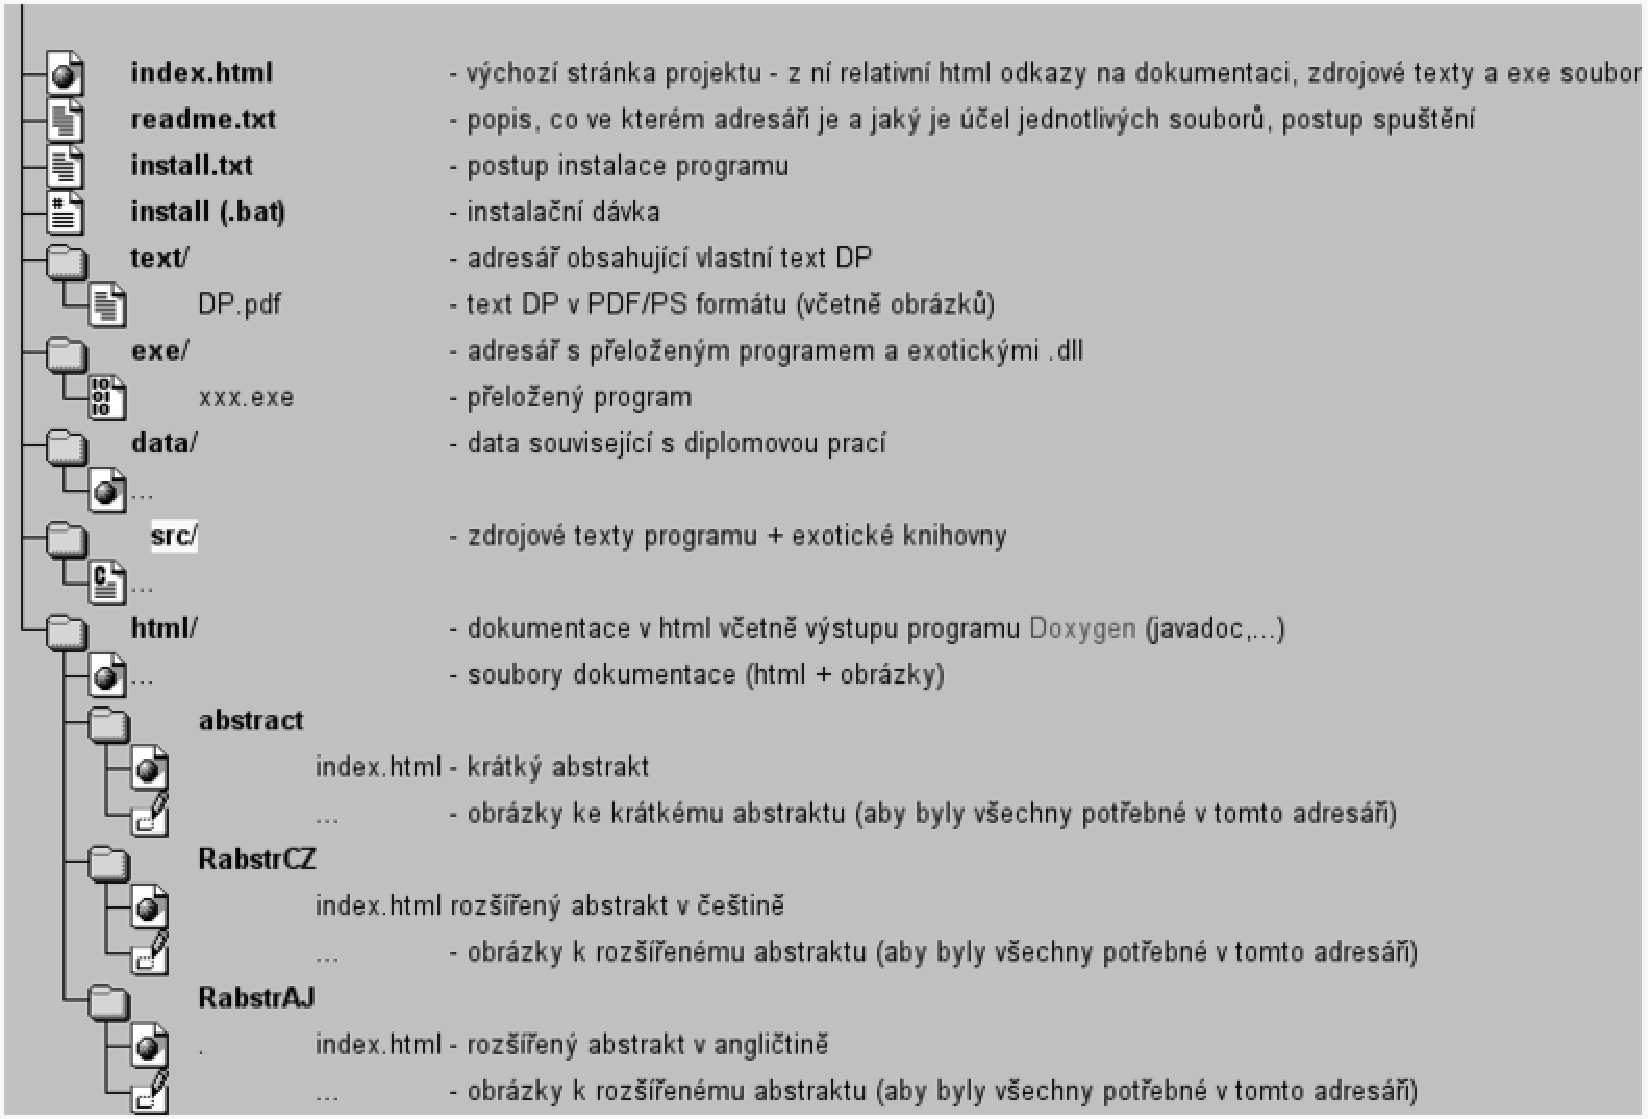
\includegraphics[width=14cm]{figures/seznamcd}
\caption{Seznam přiloženého CD --- příklad}
\label{fig:seznamcd}
\end{center}
\end{figure}

Na GNU/Linuxu si strukturu přiloženého CD můžete snadno vyrobit příkazem:\\ 
\verb|$ tree . >tree.txt|\\
Ve vzniklém souboru pak stačí pouze doplnit komentáře.

Z \textbf{README.TXT} (případne index.html apod.)  musí být rovněž zřejmé, jak programy instalovat, spouštět a jaké požadavky mají tyto programy na hardware.

Adresář \textbf{text}  musí obsahovat soubor s vlastním textem práce v PDF nebo PS formátu, který bude později použit pro prezentaci diplomové práce na WWW.

\end{document}
